% Options for packages loaded elsewhere
\PassOptionsToPackage{unicode}{hyperref}
\PassOptionsToPackage{hyphens}{url}
\PassOptionsToPackage{dvipsnames,svgnames,x11names}{xcolor}
%
\documentclass[
]{scrartcl}

\usepackage{amsmath,amssymb}
\usepackage{iftex}
\ifPDFTeX
  \usepackage[T1]{fontenc}
  \usepackage[utf8]{inputenc}
  \usepackage{textcomp} % provide euro and other symbols
\else % if luatex or xetex
  \usepackage{unicode-math}
  \defaultfontfeatures{Scale=MatchLowercase}
  \defaultfontfeatures[\rmfamily]{Ligatures=TeX,Scale=1}
\fi
\usepackage{lmodern}
\ifPDFTeX\else  
    % xetex/luatex font selection
\fi
% Use upquote if available, for straight quotes in verbatim environments
\IfFileExists{upquote.sty}{\usepackage{upquote}}{}
\IfFileExists{microtype.sty}{% use microtype if available
  \usepackage[]{microtype}
  \UseMicrotypeSet[protrusion]{basicmath} % disable protrusion for tt fonts
}{}
\makeatletter
\@ifundefined{KOMAClassName}{% if non-KOMA class
  \IfFileExists{parskip.sty}{%
    \usepackage{parskip}
  }{% else
    \setlength{\parindent}{0pt}
    \setlength{\parskip}{6pt plus 2pt minus 1pt}}
}{% if KOMA class
  \KOMAoptions{parskip=half}}
\makeatother
\usepackage{xcolor}
\setlength{\emergencystretch}{3em} % prevent overfull lines
\setcounter{secnumdepth}{5}
% Make \paragraph and \subparagraph free-standing
\ifx\paragraph\undefined\else
  \let\oldparagraph\paragraph
  \renewcommand{\paragraph}[1]{\oldparagraph{#1}\mbox{}}
\fi
\ifx\subparagraph\undefined\else
  \let\oldsubparagraph\subparagraph
  \renewcommand{\subparagraph}[1]{\oldsubparagraph{#1}\mbox{}}
\fi

\providecommand{\tightlist}{%
  \setlength{\itemsep}{0pt}\setlength{\parskip}{0pt}}\usepackage{longtable,booktabs,array}
\usepackage{calc} % for calculating minipage widths
% Correct order of tables after \paragraph or \subparagraph
\usepackage{etoolbox}
\makeatletter
\patchcmd\longtable{\par}{\if@noskipsec\mbox{}\fi\par}{}{}
\makeatother
% Allow footnotes in longtable head/foot
\IfFileExists{footnotehyper.sty}{\usepackage{footnotehyper}}{\usepackage{footnote}}
\makesavenoteenv{longtable}
\usepackage{graphicx}
\makeatletter
\def\maxwidth{\ifdim\Gin@nat@width>\linewidth\linewidth\else\Gin@nat@width\fi}
\def\maxheight{\ifdim\Gin@nat@height>\textheight\textheight\else\Gin@nat@height\fi}
\makeatother
% Scale images if necessary, so that they will not overflow the page
% margins by default, and it is still possible to overwrite the defaults
% using explicit options in \includegraphics[width, height, ...]{}
\setkeys{Gin}{width=\maxwidth,height=\maxheight,keepaspectratio}
% Set default figure placement to htbp
\makeatletter
\def\fps@figure{htbp}
\makeatother
\newlength{\cslhangindent}
\setlength{\cslhangindent}{1.5em}
\newlength{\csllabelwidth}
\setlength{\csllabelwidth}{3em}
\newlength{\cslentryspacingunit} % times entry-spacing
\setlength{\cslentryspacingunit}{\parskip}
\newenvironment{CSLReferences}[2] % #1 hanging-ident, #2 entry spacing
 {% don't indent paragraphs
  \setlength{\parindent}{0pt}
  % turn on hanging indent if param 1 is 1
  \ifodd #1
  \let\oldpar\par
  \def\par{\hangindent=\cslhangindent\oldpar}
  \fi
  % set entry spacing
  \setlength{\parskip}{#2\cslentryspacingunit}
 }%
 {}
\usepackage{calc}
\newcommand{\CSLBlock}[1]{#1\hfill\break}
\newcommand{\CSLLeftMargin}[1]{\parbox[t]{\csllabelwidth}{#1}}
\newcommand{\CSLRightInline}[1]{\parbox[t]{\linewidth - \csllabelwidth}{#1}\break}
\newcommand{\CSLIndent}[1]{\hspace{\cslhangindent}#1}

\usepackage{booktabs}
\usepackage{caption}
\usepackage{longtable}
\usepackage{colortbl}
\usepackage{array}
\usepackage{typearea}
\usepackage{lscape}
\usepackage{afterpage}
\usepackage{changepage}
\usepackage{scrlayer-scrpage}
\usepackage{soul}
\usepackage{lastpage}
\lohead{ADVANCE TRAUMA Trial Protocol}
\rohead{ClinicalTrials.gov ID NCT06321419}
\cfoot{\thepage\ of \pageref{LastPage} }
\makeatletter
\makeatother
\makeatletter
\makeatother
\makeatletter
\@ifpackageloaded{caption}{}{\usepackage{caption}}
\AtBeginDocument{%
\ifdefined\contentsname
  \renewcommand*\contentsname{Table of contents}
\else
  \newcommand\contentsname{Table of contents}
\fi
\ifdefined\listfigurename
  \renewcommand*\listfigurename{List of Figures}
\else
  \newcommand\listfigurename{List of Figures}
\fi
\ifdefined\listtablename
  \renewcommand*\listtablename{List of Tables}
\else
  \newcommand\listtablename{List of Tables}
\fi
\ifdefined\figurename
  \renewcommand*\figurename{Figure}
\else
  \newcommand\figurename{Figure}
\fi
\ifdefined\tablename
  \renewcommand*\tablename{Table}
\else
  \newcommand\tablename{Table}
\fi
}
\@ifpackageloaded{float}{}{\usepackage{float}}
\floatstyle{ruled}
\@ifundefined{c@chapter}{\newfloat{codelisting}{h}{lop}}{\newfloat{codelisting}{h}{lop}[chapter]}
\floatname{codelisting}{Listing}
\newcommand*\listoflistings{\listof{codelisting}{List of Listings}}
\makeatother
\makeatletter
\@ifpackageloaded{caption}{}{\usepackage{caption}}
\@ifpackageloaded{subcaption}{}{\usepackage{subcaption}}
\makeatother
\makeatletter
\@ifpackageloaded{tcolorbox}{}{\usepackage[skins,breakable]{tcolorbox}}
\makeatother
\makeatletter
\@ifundefined{shadecolor}{\definecolor{shadecolor}{rgb}{.97, .97, .97}}
\makeatother
\makeatletter
\makeatother
\makeatletter
\makeatother

\usepackage{hyphenat}
\usepackage{ifthen}
\usepackage{calc}
\usepackage{calculator}



\usepackage{graphicx}
\usepackage{geometry}
\usepackage{afterpage}
\usepackage{tikz}
\usetikzlibrary{calc}
\usetikzlibrary{fadings}
\usepackage[pagecolor=none]{pagecolor}


% Set the titlepage font families







% Set the coverpage font families

\ifLuaTeX
  \usepackage{selnolig}  % disable illegal ligatures
\fi
\IfFileExists{bookmark.sty}{\usepackage{bookmark}}{\usepackage{hyperref}}
\IfFileExists{xurl.sty}{\usepackage{xurl}}{} % add URL line breaks if available
\urlstyle{same} % disable monospaced font for URLs
\hypersetup{
  pdftitle={Clinical Trial Protocol},
  pdfauthor={Version 1.4.0, 2025-04-30},
  colorlinks=true,
  linkcolor={blue},
  filecolor={Maroon},
  citecolor={Blue},
  urlcolor={Blue},
  pdfcreator={LaTeX via pandoc}}

\title{Clinical Trial Protocol}
\usepackage{etoolbox}
\makeatletter
\providecommand{\subtitle}[1]{% add subtitle to \maketitle
  \apptocmd{\@title}{\par {\large #1 \par}}{}{}
}
\makeatother
\subtitle{ADVANCE TRAUMA\\
\strut \\
Effects of Advanced Trauma Life Support\textsuperscript{®} Training
Compared to Standard Care on Adult Trauma Patient Outcomes: A Cluster
Randomised Trial}
\author{Version 1.4.0, 2025-04-30}
\date{}

\begin{document}
%%%%% begin titlepage extension code


\begin{titlepage}

%%% TITLE PAGE START

% Set up alignment commands
%Page
\newcommand{\titlepagepagealign}{
\ifthenelse{\equal{center}{right}}{\raggedleft}{}
\ifthenelse{\equal{center}{center}}{\centering}{}
\ifthenelse{\equal{center}{left}}{\raggedright}{}
}


\newcommand{\titleandsubtitle}{
% Title and subtitle
{\fontsize{15}{18.0}\selectfont
{\uppercase{\nohyphens{Clinical Trial Protocol}}}\par
}%

\vspace{\betweentitlesubtitle}
{
\fontsize{20}{24.0}\selectfont
{\bfseries{\nohyphens{ADVANCE TRAUMA\\
\strut \\
Effects of Advanced Trauma Life Support\textsuperscript{®} Training
Compared to Standard Care on Adult Trauma Patient Outcomes: A Cluster
Randomised Trial}}}\par
}}
\newcommand{\titlepagetitleblock}{
\rule{\textwidth}{0.4pt} % Thin horizontal rule
\vspace{0.025\textheight} % Whitespace between the top rules and title

\titleandsubtitle

\vspace{0.025\textheight} 
\rule{0.3\textwidth}{0.4pt} % Short horizontal rule under the title
}
\newcommand{\authorstyle}[1]{{\Large{#1}}}

\newcommand{\affiliationstyle}[1]{{\large{#1}}}

\newcommand{\titlepageauthorblock}{
{\authorstyle{\nohyphens{Version 1.4.0, 2025-04-30}\\}}
}

\newcommand{\titlepageaffiliationblock}{
\hangindent=1em
\hangafter=1
{\affiliationstyle{


\vspace{1\baselineskip} 
}}
}
\newcommand{\headerstyled}{%
{}
}
\newcommand{\footerstyled}{%
{\large{\textsc{}}}
}
\newcommand{\datestyled}{%
{}
}


\newcommand{\titlepageheaderblock}{\headerstyled}

\newcommand{\titlepagefooterblock}{
\footerstyled
}

\newcommand{\titlepagedateblock}{
\datestyled
}

%set up blocks so user can specify order
\newcommand{\titleblock}{\newlength{\betweentitlesubtitle}
\setlength{\betweentitlesubtitle}{\baselineskip}
{

{\titlepagetitleblock}
}

\vspace{0.1\textheight}
}

\newcommand{\authorblock}{{\titlepageauthorblock}

\vspace{2\baselineskip}
}

\newcommand{\affiliationblock}{{\titlepageaffiliationblock}

\vspace{1pt}
}

\newcommand{\logoblock}{}

\newcommand{\footerblock}{}

\newcommand{\dateblock}{}

\newcommand{\headerblock}{}

\thispagestyle{empty} % no page numbers on titlepages


\newlength{\minipagewidth}
\setlength{\minipagewidth}{\textwidth}
\raggedright % single minipage
% [position of box][box height][inner position]{width}
% [s] means stretch out vertically; assuming there is a vfill
\begin{minipage}[b][\textheight][s]{\minipagewidth}
\titlepagepagealign
\titleblock

\authorblock

\vfill

\logoblock

\footerblock
\par

\end{minipage}\ifthenelse{\equal{}{right} \OR \equal{}{leftright} }{
\hspace{\B}
\vrulecode}{}
\clearpage
%%% TITLE PAGE END
\end{titlepage}
\setcounter{page}{1}

%%%%% end titlepage extension code
\ifdefined\Shaded\renewenvironment{Shaded}{\begin{tcolorbox}[sharp corners, interior hidden, borderline west={3pt}{0pt}{shadecolor}, boxrule=0pt, breakable, frame hidden, enhanced]}{\end{tcolorbox}}\fi

\renewcommand*\contentsname{Table of contents}
{
\hypersetup{linkcolor=}
\setcounter{tocdepth}{3}
\tableofcontents
}
\newpage{}

\hypertarget{visual-abstract}{%
\section{Visual abstract}\label{visual-abstract}}

\begin{figure}

{\centering \includegraphics{../shared-assets/visual-abstract-small.png}

}

\caption{Visual abstract}

\end{figure}

\newpage{}

\hypertarget{administrative-information}{%
\section{Administrative information}\label{administrative-information}}

\hypertarget{changelog}{%
\subsection{Changelog}\label{changelog}}

\begin{longtable}[]{@{}
  >{\raggedright\arraybackslash}p{(\columnwidth - 4\tabcolsep) * \real{0.1000}}
  >{\raggedright\arraybackslash}p{(\columnwidth - 4\tabcolsep) * \real{0.1500}}
  >{\raggedright\arraybackslash}p{(\columnwidth - 4\tabcolsep) * \real{0.7500}}@{}}
\toprule\noalign{}
\begin{minipage}[b]{\linewidth}\raggedright
Version
\end{minipage} & \begin{minipage}[b]{\linewidth}\raggedright
Date
\end{minipage} & \begin{minipage}[b]{\linewidth}\raggedright
Details
\end{minipage} \\
\midrule\noalign{}
\endhead
\bottomrule\noalign{}
\endlastfoot
1.4.0 & ? & \begin{minipage}[t]{\linewidth}\raggedright
\begin{itemize}
\tightlist
\item
  Updated systematic review results and references
\item
  Added visual abstract
\item
  Added details on the nested staircase design for measuring adherence,
  quality of life and disability
\item
  Removed return to work as a secondary outcome to be measured using the
  nested staircase design, this should be measured using the main
  stepped-wedge design
\end{itemize}
\end{minipage} \\
1.3.0 & 2024-11-15 & \begin{minipage}[t]{\linewidth}\raggedright
\begin{itemize}
\tightlist
\item
  Updated names of events in the table of procedures
\item
  Added new references
\item
  Added nested staircase design for measuring adherence, quality of
  life, disability and return to work
\item
  Updated small sample correction to be based on best available evidence
  closer to the time of analysis
\item
  Added contributors
\item
  Removed reassessment of the sample size calculation from the interim
  analysis
\item
  Revised details on measuring ATLS adherence
\end{itemize}
\end{minipage} \\
1.2.0 & 2024-08-26 & \begin{minipage}[t]{\linewidth}\raggedright
\begin{itemize}
\tightlist
\item
  Added details on measuring ATLS adherence
\item
  Clarified the section describing the consent process
\item
  Fixed minor issues with how the variables were listed
\item
  Indicated non-routinely recorded data in the list of variables
\item
  Added Administrative information section with contributors
\item
  Added CTRI registration number
\end{itemize}
\end{minipage} \\
1.1.0 & 2024-05-09 & Updated the primary outcome to in-hospital
mortality and spelling corrections. The primary outcome was updated
following a voting procedure in the Trial Management Group. \\
\end{longtable}

\hypertarget{study-identifiers}{%
\subsection{Study identifiers}\label{study-identifiers}}

\begin{itemize}
\tightlist
\item
  ClinicalTrials.gov identifier:
  \href{https://clinicaltrials.gov/ct2/show/NCT06321419}{NCT06321419}
\item
  Clinical Trials Registry - India identifier: CTRI/2024/07/071336
\end{itemize}

\hypertarget{contributors}{%
\subsection{Contributors}\label{contributors}}

The following have contributed to the design and implementation of the
trial:

\begin{longtable}[]{@{}
  >{\raggedright\arraybackslash}p{(\columnwidth - 4\tabcolsep) * \real{0.3500}}
  >{\raggedright\arraybackslash}p{(\columnwidth - 4\tabcolsep) * \real{0.4500}}
  >{\raggedright\arraybackslash}p{(\columnwidth - 4\tabcolsep) * \real{0.2000}}@{}}
\toprule\noalign{}
\begin{minipage}[b]{\linewidth}\raggedright
Name and ORCID
\end{minipage} & \begin{minipage}[b]{\linewidth}\raggedright
Affiliation
\end{minipage} & \begin{minipage}[b]{\linewidth}\raggedright
Role
\end{minipage} \\
\midrule\noalign{}
\endhead
\bottomrule\noalign{}
\endlastfoot
Martin Gerdin Wärnberg
\href{https://orcid.org/0000-0001-6069-4794}{\includegraphics[width=0.16667in,height=0.16667in]{ORCIDiD_icon16x16.png}}
& Karolinska Institutet, Stockholm, Sweden & Principal Investigator, TMG
chair and TT member \\
Girish D Bakhshi
\href{https://orcid.org/0000-0001-9542-4428}{\includegraphics[width=0.16667in,height=0.16667in]{ORCIDiD_icon16x16.png}}
& Grant Govt. Medical College \& Sir J. J. Group of Hospitals, Mumbai,
India & TMG member \\
Debojit Basak
\href{https://orcid.org/90000-0002-8378-9689}{\includegraphics[width=0.16667in,height=0.16667in]{ORCIDiD_icon16x16.png}}
& Institute of Post Graduate Medical Education \& Research and Seth
Sukhlal Karnani Memorial Hospital, Kolkata, India & TMG member \\
Abhinav Bassi
\href{https://orcid.org/0000-0003-0750-9179}{\includegraphics[width=0.16667in,height=0.16667in]{ORCIDiD_icon16x16.png}}
& The George Institute for Global Health, New Delhi, India & TMG and TT
member \\
Johanna Berg
\href{https://orcid.org/0000-0001-7553-7337}{\includegraphics[width=0.16667in,height=0.16667in]{ORCIDiD_icon16x16.png}}
& Karolinska Institutet, Stockholm, Sweden & TMG member \\
Shamita Chatterjee
\href{https://orcid.org/0000-0002-9460-108X}{\includegraphics[width=0.16667in,height=0.16667in]{ORCIDiD_icon16x16.png}}
& Institute of Post Graduate Medical Education \& Research and Seth
Sukhlal Karnani Memorial Hospital, Kolkata, India & TMG member \\
Kapil Dev Soni
\href{https://orcid.org/0000-0003-1214-4119}{\includegraphics[width=0.16667in,height=0.16667in]{ORCIDiD_icon16x16.png}}
& All India Institute of Medical Sciences, New Delhi, India & TMG
member \\
Karla Hemming
\href{https://orcid.org/0000-0002-2226-6550}{\includegraphics[width=0.16667in,height=0.16667in]{ORCIDiD_icon16x16.png}}
& University of Birmingham, Birmingham, UK & TMG member \\
Vivekanand Jha
\href{https://orcid.org/0000-0002-8015-9470}{\includegraphics[width=0.16667in,height=0.16667in]{ORCIDiD_icon16x16.png}}
& The George Institute for Global Health, New Delhi, India & TMG
member \\
Jessica Kasza
\href{https://orcid.org/0000-0002-8940-0136}{\includegraphics[width=0.16667in,height=0.16667in]{ORCIDiD_icon16x16.png}}
& Monash University, Melbourne, Australia & External statistician \\
Monty Khajanchi
\href{https://orcid.org/0000-0002-0898-6391}{\includegraphics[width=0.16667in,height=0.16667in]{ORCIDiD_icon16x16.png}}
& King Edward Memorial Hospital, Mumbai, India & TMG and TT member \\
James Martin
\href{https://orcid.org/0000-0002-6949-4200}{\includegraphics[width=0.16667in,height=0.16667in]{ORCIDiD_icon16x16.png}}
& University of Birmingham, Birmingham, UK & External statistician \\
Anurag Mishra
\href{https://orcid.org/0000-0002-2302-0632}{\includegraphics[width=0.16667in,height=0.16667in]{ORCIDiD_icon16x16.png}}
& Maulana Azad Medical College, New Delhi, India & TMG member \\
Samriddhi Ranjan
\href{https://orcid.org/0000-0002-4277-6662}{\includegraphics[width=0.16667in,height=0.16667in]{ORCIDiD_icon16x16.png}}
& The George Institute for Global Health, New Delhi, India & TMG and TT
member \\
Anna Olofsson
\href{https://orcid.org/0000-0002-9460-108X}{\includegraphics[width=0.16667in,height=0.16667in]{ORCIDiD_icon16x16.png}}
& Karolinska Institutet & Trial Statistician, TMG member \\
Nobhojit Roy
\href{https://orcid.org/0000-0003-2022-7416}{\includegraphics[width=0.16667in,height=0.16667in]{ORCIDiD_icon16x16.png}}
& The George Institute for Global Health, New Delhi, India & TMG and TT
member \\
Rajdeep Singh
\href{https://orcid.org/0000-0001-6593-2624}{\includegraphics[width=0.16667in,height=0.16667in]{ORCIDiD_icon16x16.png}}
& Maulana Azad Medical College, New Delhi, India & TMG member \\
Lovisa Strömmer
\href{https://orcid.org/0000-0001-5424-7111}{\includegraphics[width=0.16667in,height=0.16667in]{ORCIDiD_icon16x16.png}}
& Karolinska Institutet, Stockholm, Sweden & TMG member \\
Li Felländer-Tsai
\href{https://orcid.org/0000-0003-0693-6080}{\includegraphics[width=0.16667in,height=0.16667in]{ORCIDiD_icon16x16.png}}
& Karolinska Institutet, Stockholm, Sweden & TMG member \\
\end{longtable}

Abbreviations: TMG, Trial Management Group; TT, Trial Team.

\newpage{}

\hypertarget{synopsis}{%
\section{Synopsis}\label{synopsis}}

\textbf{Title} Effects of Advanced Trauma Life
Support\textsuperscript{®} Training Compared to Standard Care on Adult
Trauma Patient Outcomes: A Cluster Randomised Trial

\textbf{Rationale} Trauma is a massive global health issue. Many
training programmes have been developed to help physicians in the
initial management of trauma patients. Among these programmes, Advanced
Trauma Life Support\textsuperscript{®} (ATLS\textsuperscript{®}) is the
most popular, having trained over one million physicians worldwide.
Despite its widespread use, there are no controlled trials showing that
ATLS\textsuperscript{®} improves patient outcomes. Multiple systematic
reviews emphasise the need for such trials.

\textbf{Aim} To compare the effects of ATLS\textsuperscript{®} training
with standard care on outcomes in adult trauma patients.

\textbf{Primary Outcome} In-hospital mortality within 30 days of arrival
at the emergency department.

\textbf{Trial Design} Batched stepped-wedge cluster randomised trial in
India.

\textbf{Trial Population} Adult trauma patients presenting to the
emergency department of a participating hospital.

\textbf{Sample Size} 30 clusters and 4320 patients.

\textbf{Eligibility Criteria}

\emph{Hospitals} are secondary or tertiary hospitals in India that admit
or refer/transfer for admission at least 400 patients with trauma per
year.

\emph{Clusters} are one or more units of physicians providing initial
trauma care in the emergency department of tertiary hospitals in India.

\emph{Patients participants} are adult trauma patients who presents to
the emergency department of participating hospitals and are admitted or
transferred for admission.

\textbf{Intervention} The intervention will be ATLS\textsuperscript{®}
training, a proprietary 2.5 day course teaching a standardised approach
to trauma patient care using the concepts of a primary and secondary
survey. Physicians will be trained in an accredited
ATLS\textsuperscript{®} training facility in India.

\textbf{Ethical Considerations} We will use an opt-out consent approach
for collection of routinely recorded data. We will obtain informed
consent for collection of non-routinely recorded data, such as quality
of life and disability outcomes. Patients who are unconscious or lack a
legally authorized representative will be included under a waiver of
informed consent. Note that consent here refers to consent to data
collection.

\textbf{Trial Period} February 2025, to October 2029

\newpage{}

\hypertarget{background-and-rationale}{%
\section{Background and rationale}\label{background-and-rationale}}

Each year, 4.3 million people die from trauma\textsuperscript{1}. Among
people aged 10-24 and 25-49 years trauma is the largest cause of
disability adjusted life years\textsuperscript{2}. Most deaths from
trauma occur within the first 24-48 hours\textsuperscript{3}. Traumatic
brain injury and exsanguination are the most common causes of trauma
deaths\textsuperscript{4,5}. Most preventable trauma deaths are caused
by clinical judgement errors during initial resuscitation or early care
including airway management and haemorrhage control, even though the
deaths occur later during the hospital stay\textsuperscript{4,6}.

Several trauma life support training programmes have been developed to
improve the early management of patients in the hospital by providing a
structured framework for assessment and
treatment\textsuperscript{7--11}. The proprietary Advanced Trauma Life
Support\textsuperscript{®} (ATLS\textsuperscript{®}) is the most
established trauma life support training programme and more than one
million physicians in over 80 countries have been trained in the
programme since the first course in 1978\textsuperscript{12}. In the US
and many other countries training in ATLS\textsuperscript{®} is
virtually mandatory for trauma care physicians\textsuperscript{13}.
Uptake in low- and middle income countries (LMIC) has been slow,
potentially due to high costs\textsuperscript{9}.

There are three randomised studies showing that ATLS\textsuperscript{®}
improves knowledge and clinical skills\textsuperscript{14--16}, but
there are no randomised controlled trials or high-quality
quasi-experimental trials indicating that ATLS\textsuperscript{®}
improves patient outcomes\textsuperscript{7,8,10,11,17}. We conducted an
updated systematic review (unpublished), and estimated a pooled risk
ratio of 0.76 (95\% CI 0.57; 1.01) from 12 heterogeneous
(I\textsuperscript{2} 0.9) observational studies on the effect of ATLS
on mortality (see Figure~\ref{fig-forest-plot})\textsuperscript{18--29}.

We conducted a pilot cluster randomised controlled trial
(ClinicalTrials.gov NCT05417243) between April 2022 and February 2023 as
part of our network grant to assess the feasibility of a full scale
trial. We published the protocol for this pilot
study\textsuperscript{30}. Our pilot study enrolled 376 patients from
seven hospitals across India (unpublished data) and shows that it is
feasible to conduct the proposed trial with a high percentage of
patients consenting to out of hospital follow up (78\%), low loss to
follow-up rate (1\%), and low missingness in key variables (mean 0.8\%).

To involve patients and the public in the planning of this trial we
conducted 19 semi-structured interviews with trauma patients,
caregivers, and community representatives (unpublished data). The aim of
these interviews was to understand their views on the trial and
important outcomes and the interviews showed high acceptability of our
research and emphasised the importance of better recovery before
discharge and functional outcomes at and after discharge, including
pain, mobility and self-care activities. The interviews also highlighted
return to work as an important outcome.

\hypertarget{updated-systematic-review}{%
\subsection{Updated systematic review}\label{updated-systematic-review}}

We perform systematic literature searches in collaboration with the
Karolinska Institutet University Library, using Medline, Embase,
Cochrane, Web of Science, Global Health, CINAHL and Google Scholar
databases (PROSPERO ID CRD42022373977). The last search was conducted on
January 22, 2025. We developed the search strategy in Medline (Ovid),
limited the search to English language articles, searched all databases
from inception, and screened a total of 10,429 records. We used a random
effects model to pool estimates across studies.

\begin{figure}

{\centering \includegraphics[width=5.81in,height=\textheight]{forest-plot.png}

}

\caption{\label{fig-forest-plot}Summary of the updated system review.
The forest plot shows the effect of ATLS on mortality. Abbreviations:
RR, risk ratio; CI, confidence interval; ATLS, Advanced Trauma Life
Support; I\textsuperscript{2}, heterogeneity.}

\end{figure}

\hypertarget{benefit-risk-evaluation}{%
\section{Benefit-risk evaluation}\label{benefit-risk-evaluation}}

The direct risks includes integrity violations and data leakage. We will
mitigate these risks by employing rigorous data collection and storage
mechanisms. The procedures that we will use to collect data will be
direct observation of care, routine physical examinations,
questionnaires, and extraction of already collected data from patient
records, which are often seen as involving only minimal risk.

The long-term risks of the research and the risk that the research will
be used in detrimental ways are minimal. Our trial will assess the
effect of Advanced Trauma Life Support\textsuperscript{®}
(ATLS\textsuperscript{®}) on patient outcomes. Training in
ATLS\textsuperscript{®} is standard in many health care systems and it
is unlikely that training physicians in this programme induces any harm
to participants.

We consider these risks weighed up by the potential direct benefit for
the participants in the intervention phase, if ATLS\textsuperscript{®}
is found to improve patient outcomes, and by the potential for improved
care for the trauma patient population.

\hypertarget{trial-aim}{%
\section{Trial aim}\label{trial-aim}}

To compare the effects of ATLS\textsuperscript{®} training with standard
care on outcomes in adult trauma patients.

\hypertarget{regulatory-approvals-and-trial-registration}{%
\section{Regulatory approvals and trial
registration}\label{regulatory-approvals-and-trial-registration}}

We will submit this trial to the Health Ministry Screening Committee at
the Indian Council for Medical Research for their approval. We will
apply for ethical approvals from each participating hospital, The George
Institute for Global Health in India and the Swedish Ethical Review
Authority. We will register this trial with Clinical Trials
Registry-India and ClinicalTrials.gov.

\hypertarget{trial-design-and-procedures}{%
\section{Trial design and
procedures}\label{trial-design-and-procedures}}

\hypertarget{overall-trial-design}{%
\subsection{Overall trial design}\label{overall-trial-design}}

We will conduct a batched stepped-wedge cluster randomised controlled
trial (see Figure~\ref{fig-trial-design}). The stepped-wedge trial is a
uni-directional cross-over trial but the time point when clusters
cross-over from standard care to the intervention is
randomised\textsuperscript{31}. Each cluster will be at least one unit
of physicians performing initial resuscitation of trauma patients in the
emergency department of tertiary hospitals in India. The number of units
that we will train in each hospital will depend on the sizes of these
units and the volumes of patients that they see. If more than one unit
is trained in the same hospital these units will be considered one unit
for the purpose of randomisation. We choose this approach for two
reasons: 1) it will not be logistically or financially feasible to train
all physician in a given hospital; and 2) we need to balance cluster
size with the number of clusters. We will conduct this trial in India
because physicians providing initial trauma care in India are so far not
routinely trained in ATLS\textsuperscript{®} or similar programmes.

We will roll out the interventions to 30 clusters over six batches, so
there will be five clusters in each batch. The clusters in each batch
will be randomised to one of five implementation sequences, with one
hospital randomised to each implementation sequence. All clusters will
transition through three phases, first a standard care phase, then a one
month transition phase during which the training is delivered, and
finally an intervention phase, for a total of 13 months. The
implementation sequence determines how long the phases of standard care
and intervention are. Patient participants will be followed up for a
total of three months.

Within the main stepped-wedge design, we will nest a staircase design to
measure a range of secondary outcomes (see
Figure~\ref{fig-nested-staircase-design}). The staircase design will
include a random subset of patients presenting during the three months
preceding the transition phase, and the three months following the
transition phase.

\hypertarget{design-justification}{%
\subsection{Design justification}\label{design-justification}}

We use the cluster randomised design because the intervention cannot be
randomised at the individual patient level. We use the stepped-wedge
design for two reasons. First, this design is statistically more
efficient than the parallel cluster design when the number of clusters
is limited\textsuperscript{32}. In this trial, the number of clusters is
limited because of the costs associated with ATLS\textsuperscript{®}
training and the available slots for ATLS\textsuperscript{®} training in
India. Second, the stepped-wedge design is likely to enhance
participation and engagement because all clusters receive the
intervention. The batched stepped-wedge design further improves
feasibility as it does not require all clusters to start at the same
time, and it is robust to potential delays in cluster
recruitment\textsuperscript{33}. We nest a staircase design within the
main design because some of the secondary outcomes will be considerably
more labour intensive to collect than the primary outcome, and
collecting these for all patient participants would be unfeasible.

\begin{figure}

{\centering \includegraphics[width=5.9in,height=\textheight]{trial-design-figure-30-clusters-5-sequences-6-batches-6-batches-overlap-4-min-standard-care-4-min-intervention-1-transition-months-0-transition-overlap.0-staircase-months.png}

}

\caption{\label{fig-trial-design}Trial design. Lines represent the
duration of patient enrolment across clusters and phases. Clusters will
be sequentially allocated to a batch based on when they enter the study.
Within each batch clusters will then be randomised to an intervention
implementation sequence.}

\end{figure}

\begin{figure}

{\centering \includegraphics[width=5.9in,height=\textheight]{trial-design-figure-30-clusters-5-sequences-6-batches-6-batches-overlap-4-min-standard-care-4-min-intervention-1-transition-months-0-transition-overlap.3-staircase-months.png}

}

\caption{\label{fig-nested-staircase-design}Nested staircase design. The
design includes a random subset of patients presenting during the three
months preceding the transition phase, and the three months following
the transition phase.}

\end{figure}

\hypertarget{eligibility-criteria}{%
\subsection{Eligibility criteria}\label{eligibility-criteria}}

Our trial include eligibility criteria on three levels: hospitals,
clusters and patient participants. We include eligibility on both the
hospital and cluster level to facilitate the screening process.

\hypertarget{hospital-selection}{%
\subsection{Hospital selection}\label{hospital-selection}}

Hospitals will be secondary or tertiary hospitals providing trauma care
in India. Hospital will be the unit of randomisation.

\hypertarget{inclusions-criteria}{%
\subsubsection{Inclusions criteria}\label{inclusions-criteria}}

\textbf{Hospitals} must meet the following criteria:

\begin{itemize}
\tightlist
\item
  admit or refer/transfer for admission at least 400 patients with
  trauma per year or 35 patients with trauma per month for at least the
  last six months;
\item
  provide surgical and orthopaedic emergency services around the clock;
  and
\item
  have at most 25\% of physicians providing initial trauma care trained
  in a formalised trauma life support training programme, like
  ATLS\textsuperscript{®} or Primary Trauma Care (PTC).
\end{itemize}

\hypertarget{exclusion-criteria}{%
\subsubsection{Exclusion criteria}\label{exclusion-criteria}}

\textbf{Hospitals} are excluded if they meet any of the following
criteria:

\begin{itemize}
\tightlist
\item
  the hospital of the cluster implements a formalised trauma life
  support training programme \footnote{These include but are not limited
    to the National Emergency Life Support (NELS) programme, the Basic
    Trauma Life Support (BTLS) programme, the Pre-Hospital Trauma Life
    Support (PHTLS) programme, the Trauma Nursing Core Course (TNCC) and
    the Advanced Trauma Care for Nurses (ATCN) programme.} during the
  trial period; or
\item
  the hospital of the cluster plan to implement or implements other
  major interventions\footnote{These include but are not limited to
    implementing of a trauma team approach, opening a trauma centre and
    implementing a trauma quality improvement programme.} that affects
  trauma care during the trial period.
\end{itemize}

\hypertarget{screening}{%
\subsubsection{Screening}\label{screening}}

The trial management group will compile a list of hospitals with
potentially eligible clusters and reach out to them to assess their
interest in participating in the trial. We will then screen hospitals
for eligibility based on the criteria above, using a two-step procedure.
First, we will approach hospitals to complete an initial hospital
screening instrument (see Appendix
Section~\ref{sec-appendix-hospital-screening-instrument}). We will then
discuss each eligible hospital individually in the Trial Management
Group before deciding whether to include it in the trial. We have this
discussion because we strive to include hospitals that to a large extent
conducts primary resuscitation of trauma patients, rather than hospitals
that primarily receives transferred patients from other hospitals, but
this is difficult to formalise in the eligibility criteria. We will then
perform a more in-depth interview with selected hospitals (See Appendix
Section~\ref{sec-appendix-hospital-screening-interview-instrument}). To
avoid excluding centres we will also discuss plans to implement other
potentially competing interventions during the trial period, and take
these plans into account when assigning clusters to batches. For
example, we are aware of the ongoing implementation of the National
Emergency Life Support (NELS) programme in India, and will therefore not
include hospitals that plan to implement this programme during the trial
period. All screening steps and decisions will be logged using
REDCap\textsuperscript{34,35}.

\hypertarget{cluster-selection}{%
\subsection{Cluster selection}\label{cluster-selection}}

Clusters are one or more units of physicians providing initial trauma
care in the emergency department of secondary or tertiary hospitals in
India. These units already exist in the hospitals and rotate through the
emergency department on specific days of the week.

\hypertarget{inclusion-criteria}{%
\subsubsection{Inclusion criteria}\label{inclusion-criteria}}

\textbf{Clusters} must meet the following criteria:

\begin{itemize}
\tightlist
\item
  admits or refers/transfers for admission at least 12 patients with
  trauma per month for at least the last six months; and
\item
  no more than 25\% of physicians providing initial trauma care trained
  in a formalised trauma life support training programme.
\end{itemize}

\hypertarget{screening-1}{%
\subsubsection{Screening}\label{screening-1}}

The screening of clusters is part of the hospital screening process.

\hypertarget{patient-participants-selection}{%
\subsection{Patient participants
selection}\label{patient-participants-selection}}

Patient participants are adult trauma patients who presents to the
emergency department of participating hospitals and are admitted or
transferred for admission.

\hypertarget{inclusion-criteria-1}{%
\subsubsection{Inclusion criteria}\label{inclusion-criteria-1}}

\textbf{Patients participants} must meet the following criteria:

\begin{itemize}
\tightlist
\item
  age of at least 15 years;
\item
  trauma occurred less than 48 hours before arrival at the hospital;
\item
  present to the emergency department of participating hospitals, with a
  history of trauma defined as having any of the reasons listed in the
  International Classification of Diseases chapter XX as the reason for
  presenting;
\item
  admitted, or died between arrival at the hospital and admission, or
  referred/transferred from the emergency department of a participating
  hospital to another hospital for admission; and
\item
  managed by a participating cluster in the emergency department.
\end{itemize}

\hypertarget{exclusion-criteria-1}{%
\subsubsection{Exclusion criteria}\label{exclusion-criteria-1}}

\textbf{Patients participants} are excluded if they meet the following
criteria:

\begin{itemize}
\tightlist
\item
  present with isolated limb injuries; or
\item
  are directly admitted to a ward without being seen by a physician in
  the emergency department.
\end{itemize}

\hypertarget{screening-2}{%
\subsubsection{Screening}\label{screening-2}}

Clinical research coordinators will screen patient participants either
as they arrive to the emergency department or using emergency department
registers. The patients or their representatives will receive written
information about the study before they are discharged, including about
their right to opt out at any time before final analysis. Phone numbers
for out of hospital follow up will be extracted from the emergency
department registers, and will be securely held only by the clinical
research coordinators at each sites.

\hypertarget{withdrawal-criteria}{%
\subsubsection{Withdrawal criteria}\label{withdrawal-criteria}}

Patient participants can choose to withdraw their consent for collection
of non-routinely recorded data at any time before the final analysis. If
they withdraw their consent for this data collection the clinical
research coordinator will not collect any more of this data, which also
means that no further follow-ups will be conducted. They can also choose
to have the data already collected about them removed from the trial at
any time before final analysis of the data. Withdrawal of consent or
removal of data from the trial will not affect their care in any way. If
the patient participant withdraws consent, follow-up of this participant
will be performed according to the participating hospitals routine.

\hypertarget{procedures}{%
\subsection{Procedures}\label{procedures}}

Table~\ref{tbl-procedures-baseline} shows an overview of trial
procedures before and during patient admission, and
Table~\ref{tbl-procedures-followup} shows an overview of trial follow-up
procedures. Clinical research coordinators will follow up patients daily
until discharge to capture injury information. They will also follow up
patients at 24 hours, 30 days and 90 days after arrival to the emergency
department to capture mortality outcomes, and at 30 days and 90 days
after arrival to the emergency department to capture functional outcomes
and return to work. If patient participants are discharged before any of
these follow-up time points, clinical research coordinators will follow
up patients by phone.

\hypertarget{tbl-procedures-baseline}{}
\setlength{\LTpost}{0mm}
\begin{longtable}{lllll}
\caption{\label{tbl-procedures-baseline}Overview of trial procedures before and during patient admission }\tabularnewline

\toprule
Procedure & Screening & Consenting & Initial assessment & In-hospital care \\ 
\midrule\addlinespace[2.5pt]
Eligibility criteria & √ &  &  &  \\ 
Study information\textsuperscript{\textit{1}} &  & √ &  &  \\ 
Informed consent\textsuperscript{\textit{1}} &  & √ &  &  \\ 
Baseline data collection &  &  & √ &  \\ 
Prehospital data collection &  &  & √ &  \\ 
ATLS adherence\textsuperscript{\textit{2}} &  &  & √ &  \\ 
ED data collection\textsuperscript{\textit{3}} &  &  & √ &  \\ 
Hospital data collection &  &  &  & √ \\ 
Surgery data collection &  &  &  & √ \\ 
Imaging data collection &  &  &  & √ \\ 
Transfusion data collection &  &  &  & √ \\ 
Injury data collection &  &  &  & √ \\ 
Mortality data collection &  &  &  & √ \\ 
Assessment of safety events &  &  &  & √ \\ 
\bottomrule
\end{longtable}
\begin{minipage}{\linewidth}
\textsuperscript{\textit{1}}Clinical research coordinators will inform patient participants about the study, including that they are free to withdraw their data from the study at any time, and approach them for informed consent for collection of non-routinely recorded data in person or telephonically.\\
\textsuperscript{\textit{2}}ATLS adherence will be assessed by observing the care provided to a random sample of patient participants.\\
\textsuperscript{\textit{3}}Emergency Department\\
\end{minipage}

\hypertarget{tbl-procedures-followup}{}
\setlength{\LTpost}{0mm}
\begin{longtable}{llll}
\caption{\label{tbl-procedures-followup}Overview of trial follow-up procedures }\tabularnewline

\toprule
Procedure & Within 7 days of discharge & 30 days & 90 days \\ 
\midrule\addlinespace[2.5pt]
Mortality data collection\textsuperscript{\textit{1}} & √ & √ & √ \\ 
EQ-5D/WHODAS & √ & √ & √ \\ 
Return to work &  & √ & √ \\ 
End of study &  &  & √ \\ 
\bottomrule
\end{longtable}
\begin{minipage}{\linewidth}
\textsuperscript{\textit{1}}Will be ascertained daily from when the patient participant arrive to hospital until they leave the hospital, are discharged or die.\\
\end{minipage}

\hypertarget{biological-sampling-procedures}{%
\subsection{Biological sampling
procedures}\label{biological-sampling-procedures}}

This trial does not include biological sampling.

\hypertarget{end-of-trial}{%
\subsection{End of trial}\label{end-of-trial}}

The trial ends when the last patient participant has completed the last
follow-up. The trial may be prematurely terminated if it this is
necessary for safety reasons affecting the risk-benefit balance or if
the recruitment of subjects cannot be met within reasonable time limits.
If the trial is prematurely terminated or suspended, the investigator
should immediately inform the subjects about this and ensure appropriate
treatment and follow-up. Decisions on premature termination are taken by
the joint Trial Steering and Data Monitoring Committee and Trial
Management Group.

\hypertarget{intervention-and-control-treatment}{%
\subsection{Intervention and control
treatment}\label{intervention-and-control-treatment}}

The intervention will be ATLS\textsuperscript{®} training. The control
will be standard care, meaning no formal trauma life support training.
We will train the physicians that initially resuscitate and provide
trauma care during the first hour after patient arrival at the emergency
department. These physicians can be casualty medical officers, surgical
residents, or emergency medicine residents, depending on the setup at
each participating centre. The training will occur during the transition
phase in each cluster. Our experience from our pilot study is that study
sites adhere to the training slot alloted to them through the trial, so
we judge the risk of clusters implementing ATLS\textsuperscript{®}
before their randomised implementation sequence as very low.

We will train the number units of physicians needed to reach the
required patient sample size, but estimate that this will require
training an average of ten physicians per hospital, which on average
should be mean that we can train one to two units per hospital. This is
possible because many hospitals in India organise physicians staffing
their emergency departments in units, and the physicians in the same
unit work together in the emergency department on the same days of the
week. We will therefore collect data only on the days when these units
work. The units selected to constitute a cluster from each hospital will
be a convenience sample out of all eligible units in those hospitals.

\textbf{Advanced Trauma Life Support\textsuperscript{®}
(ATLS\textsuperscript{®})\textsuperscript{12}} is a proprietary 2.5 day
course teaching a standardised approach to trauma patient care using the
concepts of a primary and secondary survey. The programme was developed
by the Committee of Trauma of the American College of Surgeons. The
course includes intial treatment and resuscitation, triage and
interfacility transfers. Leaning is based on practical scenario-driven
skill stations, lectures and includes a final performance proficiency
evaluation. Physicians will be trained in an accredited
ATLS\textsuperscript{®} training facility in India. We will assess
adherence to ATLS principles before and after implementing ATLS
training.

\textbf{Standard care} varies across hospitals in India, but trauma
patients are initially managed by casualty medical officers, surgical
residents, or emergency medicine residents. They are mainly first- or
second-year residents who resuscitate patients, perform interventions
and refer patients for imaging or other investigations. Compared with
other settings where a trauma team approach is adopted, nurses and other
healthcare professionals are only involved to a limited extent during
the initial management.

\hypertarget{description-of-investigational-medicinal-products}{%
\subsubsection{Description of investigational medicinal
products}\label{description-of-investigational-medicinal-products}}

This trial does not include any investigational medicinal products.

\hypertarget{auxiliary-medicinal-products}{%
\subsubsection{Auxiliary medicinal
products}\label{auxiliary-medicinal-products}}

This trial does not include any auxiliary medicinal products.

\hypertarget{concomitant-use-of-other-medications-or-treatments}{%
\subsubsection{Concomitant use of other medications or
treatments}\label{concomitant-use-of-other-medications-or-treatments}}

Other than implementing another formalised trauma life support training
programme or other major interventions to change the care of trauma
patients as specified in the exclusion criteria, concomitant use of
other medications and treatments may be provided at the discretion of
the investigators and will not be considered an exclusion criterion.

\hypertarget{randomisation}{%
\subsection{Randomisation}\label{randomisation}}

We will assign clusters to batches as they are found to be eligible and
receive ethical approval. Batches will include clusters from hospitals
in different regions to optimize trial logistics. We will randomise the
clusters alloted to each batch to the different intervention
implementation sequences within that batch\footnote{Randomisation will
  be done using bespoke code from previous trials.}. We will balance the
randomisation within each batch on cluster size, defined as monthly
volume of eligible patient participants, using covariate constrained
randomisation. The cluster sizes are expected to vary between 12 and 20
patients per month, based on our previous experiences. We will conceal
the randomisation order for as long as it is logistically possible,
considering that arrangements for sending physicians to
ATLS\textsuperscript{®} training need to be made in advance.

\hypertarget{blinding}{%
\subsection{Blinding}\label{blinding}}

It is not possible to blind a stepped-wedge trial, because all clusters
receive the intervention.

\hypertarget{treatment-after-trial-end}{%
\subsection{Treatment after trial end}\label{treatment-after-trial-end}}

When the trial ends, the intervention will have been implemented in all
clusters.

\hypertarget{outcomes}{%
\subsection{Outcomes}\label{outcomes}}

\hypertarget{primary-outcome}{%
\subsubsection{Primary outcome}\label{primary-outcome}}

The primary outcome will be in-hospital mortality within 30 days of
arrival at the emergency department. Clinical research coordinators will
extract information on death from patient hospital records. If the
patient has been transferred to another hospital, the clinical research
coordinators will collect data on this outcome by calling the patient or
a patient representative, or by contacting the hospital to which the
patient was transferred. Data on this outcome will be collected
continuously during the trial.

\hypertarget{secondary-outcomes}{%
\subsubsection{Secondary outcomes}\label{secondary-outcomes}}

\hypertarget{collected-using-the-main-stepped-wedge-design}{%
\paragraph{Collected using the main stepped-wedge
design}\label{collected-using-the-main-stepped-wedge-design}}

\begin{itemize}
\tightlist
\item
  All cause mortality within 24 hours, 30 days and three months of
  arrival at the emergency department. Data on this outcome will be
  collected in the same way as for the primary outcome.
\item
  Length of emergency department stay. Data on this outcome will be
  collected from patient hospital records.
\item
  Length of hospital stay. Data on this outcome will be collected from
  patient hospital records.
\item
  Intensive care unit admission. Data on this outcome will be collected
  from patient hospital records.
\item
  Length of intensive care unit stay. Data on this outcome will be
  collected from patient hospital records.
\item
  Return to work at 30 days and three months after arrival at the
  emergency department. Data on this outcome will be collected in person
  if the patient is still in hospital, or by phone if the patient has
  been discharged.
\end{itemize}

\hypertarget{collected-using-the-nested-staircase-design}{%
\paragraph{Collected using the nested staircase
design}\label{collected-using-the-nested-staircase-design}}

\begin{itemize}
\tightlist
\item
  Adherence to ATLS\textsuperscript{®} principles during initial patient
  resuscitation, up to one hour after the physician has first seen the
  patient. This assessment will be done using a 14 item checklist
  covering the key steps of the ATLS\textsuperscript{®} primary survey,
  which was modelled based on previous work on ATLS\textsuperscript{®}
  adherence\textsuperscript{36}. We will consider completion of all 14
  steps as 100\% adherence. The clinical research coordinators
  collecting the data will be trained by the trial team to do this,
  prior to the start of the trial. We will collect this data by
  observing the care of a random sample of patients. The sampling will
  be designed as a nested staircase design.
\item
  Quality of life within seven days of discharge, and at 30 days and
  three months of arrival at the emergency department, measured by the
  official and validated translations of the EQ5D3L. Data on this
  outcome will be collected in person if the patient is still in
  hospital, or by phone if the patient has been discharged. We will
  collect this data using a nested staircase design.
\item
  Disability within seven days of discharge, and at 30 days and three
  months of arrival at the emergency department, assessed using the WHO
  Disability Assessment Schedule 2.0 (WHODAS 2.0). Data on this outcome
  will be collected in person if the patient is still in hospital, or by
  phone if the patient has been discharged. This data will also be
  collected using a nested staircase design.
\end{itemize}

\hypertarget{handling-of-adverse-and-safety-events}{%
\subsection{Handling of adverse and safety
events}\label{handling-of-adverse-and-safety-events}}

\hypertarget{definitions}{%
\subsubsection{Definitions}\label{definitions}}

\hypertarget{adverse-event}{%
\paragraph{Adverse event}\label{adverse-event}}

Any untoward medical occurrence in a clinical trial subject and, which
does not necessarily have a causal relationship with the treatment, can
be an unfavorable and unintended sign (including an abnormal laboratory
discovery), symptom or disease temporally associated with the inclusion
in the trial, whether or not related to the trial.

\hypertarget{serious-adverse-event}{%
\paragraph{Serious adverse event}\label{serious-adverse-event}}

Any untoward medical occurrence in a trial participant that:

\begin{itemize}
\tightlist
\item
  leads to death
\item
  is life-threatening
\item
  requires inpatient hospitalization or prolongation of existing
  hospitalization
\item
  results in persistent or significant disability or incapacity
\item
  results in a congenital anomaly/malformation
\end{itemize}

\hypertarget{safety-event}{%
\paragraph{Safety event}\label{safety-event}}

Any unexpected serious complication that might occur as a consequence of
the trial and that are not part of the natural history of trauma.

\hypertarget{reporting-and-assessment-of-adverse-and-safety-events}{%
\subsubsection{Reporting and assessment of adverse and safety
events}\label{reporting-and-assessment-of-adverse-and-safety-events}}

In alignment with other current trials including critically ill
patients\textsuperscript{37}, we will not collect adverse events or
serious adverse events, because many of these events are expected in
this patient population and we already collect many of these events, for
example mortality, as part of our outcomes.

We will only report safety events, if they are life-threatening, prolong
hospitalisation or result in meaningful harm to the participant. We
cannot pre-define a comprehensive list of events that can be considered
safety events, but will actively assess the presence of the following
safety events:

\begin{itemize}
\tightlist
\item
  Prolonged mechanical ventilation (\textgreater{} 7 days)
\item
  Initiation of renal replacement therapy
\item
  Prolonged (\textgreater{} 2 days) or renewed (restart after at least 2
  days without) use of vasopressors such as norepinephrine or
  vasopressin
\end{itemize}

These events are considered safety events because they suggest
pulmonary, renal, septic or bleeding complications and an increase in
their occurrence following ATLS\textsuperscript{®} training could
indicate that the intervention is harmful. These events therefore need
to be tracked during the standard care phase as well as the intervention
phase, but will only be considered indicative of harm related to the
intervention if they occur more often during the intervention phase than
during the standard care phase.

We will also report any other safety events that we identify during the
trial, and the reporting of such will have to be based on the intuition
of the clinical research coordinators and local investigators. Examples
of such safety events could include missed injuries or missed
investigations, which could be suspected if certain injuries or
investigations were identified or conducted more often during the
standard care phase than during the intervention phase.

All safety events will be recorded in the Case Record Form (CRF) and
reported to the trial management team within 24 hours of its occurrence.
The trial management team will then assess if the event can be
considered related to the trial or the intervention within 24 hours of
it being reported. Events that are considered probably related will be
reported immediately to the joint Trial Steering and Data Monitoring
Committee.

\hypertarget{follow-up-of-safety-events}{%
\subsubsection{Follow up of safety
events}\label{follow-up-of-safety-events}}

All safety events should be followed up by the local investigator until
they are fully evaluated.

\hypertarget{statistics}{%
\subsection{Statistics}\label{statistics}}

\hypertarget{general-principles}{%
\subsubsection{General principles}\label{general-principles}}

We will conduct all analysis by modified intention to treat. Clusters
and observations within clusters will be considered exposed to the
intervention after the date at which the cluster was scheduled to
transition. All data will be included with the exception of the
transition phases. We will not adjust for multiplicity of analyses
because none of the secondary outcomes will be singularly more
important. However, all secondary outcomes will be interpreted with due
consideration for how all are affected by the intervention without
putting any undue emphasis on a single outcome that might be
statistically significant but where all others appear to have remained
unchanged.

We will use a two-sided significance level of 5\% and estimate 95\%
confidence intervals. The primary subgroup analyses will be based on
geographical region because demonstrating the consistency of any effect
across multiple regions will enhance the generalisibility of the
results\footnote{\textbf{Note:} Batches will not be based on regions
  because it will be logistically more feasible to include clusters from
  different regions in each batch.}. Additional subgroup analyses will
include age across the groups older adolescents (15-19 years), young
adults (20-24 years), adults (25-59 years), and older adults (60 years
and older)\textsuperscript{38}; sex; and the clinical cohorts blunt
multisytem trauma, penetrating trauma, and severe isolated traumatic
brain injury.

\hypertarget{analysis-models}{%
\subsubsection{Analysis models}\label{analysis-models}}

There are a number of requirements for the analysis model. Firstly, all
analysis will consider the clustered nature of the design. Secondly, as
the trial has only 30 clusters, it will be essential that the model
allows for a correction due to the small number of clusters. Thirdly, as
the design is a stepped-wedge study, we will adjust for temporal
confounding using categorical effects for period of the study (month).
Full details on how each of these will be undertaken, with justification
is provided below\textsuperscript{39}.

For binary outcomes, a mixed effects binomial regression with a logit
link will be used to estimate the odds ratio; and a binomial model with
identity link used to estimate the risk difference. These models will be
fitted using residual pseudo-likelihood estimation based on
linearization with subject-specific expansion (RSPL). If the binomial
model with the identity link does not converge then only a odds ratio
will be reported.

We will include fixed effects for period and a fixed effect for
intervention exposure. The primary analysis will allow for clustering by
as a random cluster and random cluster by period effect. To correct the
potential inflation of the type I error rate due to small number of
clusters, a correction for a small number of clusters will be applied,
but the correction that will be selected will be based on the best
available evidence available closer to the time, and it may differ for
the outcomes collected via the complete and incomplete designs. In a
sensitivity analysis we will explore if models with more complicated
correlation structures are a better fit to the data. These models are
not being used as our primary analysis models as there is limited
understanding as to when such models will converge and how to choose
between the various different correlation structures which might be
plausible.

To this end we will additionally fit generalised linear mixed models
(with same link functions and fixed effects as described above) to
include a discrete time decay correlation structure including a random
cluster effect with auto-regressive structure (AR(1)). To allow for the
randomisation by batches, a different secular trend will be included for
each batch (interaction between batch and period). For continuous, count
and prevalence outcomes similar model-based approaches will be used but
with appropriate links and distribution functions, using transformations
where appropriate.

\hypertarget{additional-sensitivity-analyses}{%
\subsubsection{Additional sensitivity
analyses}\label{additional-sensitivity-analyses}}

To additionally explore if the fixed period effect is both parsimonious
and adequate to represent the extent of any underlying secular trend, we
will model the time effect using a spline function. Models will also be
extended to include random cluster by intervention effects (with a
non-zero covariance term) to examine if results are sensitive to the
assumption of no intervention by cluster interaction. Models will also
be extended to include an interaction between treatment and number of
periods since first treated, to examine if there is any indication of a
relationship between duration of exposure to the intervention and
outcomes.

This will allow us to different lag effects (whereby it takes time for
the intervention to become embedded within the culture before its impact
can properly start to be realised); as well as weaning effects (whereby
the effect of the intervention starts to decrease -- or fade). This type
of analysis attempts to disentangle how some clusters end up having a
long exposure to the intervention and others have a much shorter
exposure time. A fully adjusted covariate analysis will additionally
adjust for a set of pre-specified individual-level covariates of known
prognostic importance.

\hypertarget{estimation-and-reporting-of-within-cluster-correlations}{%
\subsubsection{Estimation and reporting of within cluster
correlations}\label{estimation-and-reporting-of-within-cluster-correlations}}

We will report time adjusted within-cluster correlations for all
outcomes with 95\% confidence intervals. We will report correlations
from the different assumed correlation structures (so we will report
intra-cluster correlations (ICC); within and between-period
correlations; and within-period correlations and exponential decay). As
well as reporting correlations we will additionally report all variance
components. For all outcomes we will report correlations on the latent
scale (i.e.~proportions scale for binary outcomes) as is appropriate to
inform future sample size calculations.

\hypertarget{sample-size-calculations}{%
\subsubsection{Sample size
calculations}\label{sample-size-calculations}}

\hypertarget{main-stepped-wedge-design-and-primary-outcome}{%
\paragraph{Main stepped wedge design and primary
outcome}\label{main-stepped-wedge-design-and-primary-outcome}}

With 30 clusters across 6 batches and a total sample size of 4320 our
study has \textasciitilde90\% power across different combinations of
cluster autocorrelations (CAC) and intra-cluster correlations (ICC) to
detect a reduction in the primary outcome of in-hospital mortality
within 30 days from 20\% under standard care to 15\% after
ATLS\textsuperscript{®} training (see Figure~\ref{fig-power-curves}).
This effect is a conservative estimate and the reduction equals a risk
ratio of 0.75, which would be clinically important while also being
consistent with our pilot study and updated systematic review. We
allowed for the clustered design and assumed an ICC of 0.02, but
considered sensitivity across the range
0.01-0.05\textsuperscript{40,41}, and a CAC of 0.9 but considered
sensitivity across the range 0.8-1.0, based on our pilot study and
current guidance\textsuperscript{42--44}. We included the CAC to allow
for variation in clustering over time. We assume that each cluster will
contribute approximately 12 observations per month to the analysis,
based on our previous work.

\begin{figure}

{\centering \includegraphics[width=7.08in,height=\textheight]{./combined-power-curves.png}

}

\caption{\label{fig-power-curves}Power curves for different combinations
of cluster autocorrelations (CAC) and intra-cluster correlations (ICC).
\textbf{A)} Shows power curves assuming a reduction in the primary
outcome of in-hospital mortality within 30 days from 20\% under standard
care to 15\% after ATLS\textsuperscript{®} training. \textbf{B)} Shows
power curves assuming a reduction in the primary outcome from 10\% under
standard care to 7.5\% after ATLS\textsuperscript{®} training. Under
this scenario, we would need to increase the sample size per month to
around 30 observations to achieve 90\% powere under most combinations of
CAC and ICC.}

\end{figure}

\hypertarget{nested-staircase-design-and-secondary-outcomes}{%
\paragraph{Nested staircase design and secondary
outcomes}\label{nested-staircase-design-and-secondary-outcomes}}

The secondary outcomes that will be measured using the nested staircase
design are adherence to ATLS\textsuperscript{®} principles during
initial patient resuscitation, quality of life, and disability. The
expected effect of the intervention on each of these outcomes are an
improvement in adherence from 50\% during standard care to 70\% after
training\textsuperscript{45}, an increase in EQ5D5L health status from
70 during care to 75 after training\textsuperscript{46}, and finally a
decrease in disability from a baseline value of 25 during standard care
to 22.5 after training\textsuperscript{47}. For quality of life and
disability, these effects correspond to standardised effect sizes,
expressed as Cohen's d, of 0.5. With 30 clusters in total, six per
sequence, for a discrete time decay correlation structure, with ICCs of
0.01 to 0.15 and a CAC of 0.8, there is \textgreater80\% power to detect
an these effects by including four patients in each cluster in each
period. Accounting for loss to follow-up, we will include at least six
patients per cluster per month. These patients will be a random subset
of patients included during the staircase months. The random subset will
be selected using simple random sampling on the shift level, meaning
that the timing of the clinical research coordinator's shift will be
randomised to cover approximately eight hours during the morning,
afternoon, or night shift. Adherence to ATLS\textsuperscript{®}
principles, quality of life, and disability will be measured in all
patients included during these shifts. In each hospital, the number of
shifts that will be randomised will be determined by the volume of
patients included during the months preceding the staircase months.

\hypertarget{interim-analysis}{%
\subsubsection{Interim analysis}\label{interim-analysis}}

There will be one interim analyses after half of the batches have
completed the trial. The interim analyses will be assessed by the joint
Trial Steering and Data Monitoring Committee. The purposes of this
interim analysis will be to:

\begin{itemize}
\tightlist
\item
  assess the trial's feasibility and recommend stopping the trial if the
  trial is not feasible, for example if hospitals fail to adhere to the
  randomisation schedule or if there are substantial missing data in
  outcomes;
\item
  compare characteristics across intervention conditions to monitor for
  differential recruitment/ascertainment between intervention and
  control.
\end{itemize}

\hypertarget{quality-control-and-quality-assurance}{%
\subsection{Quality control and quality
assurance}\label{quality-control-and-quality-assurance}}

The George Institute for Global Health - India will ensure proper
conduct of the trial through quality control measures including on-site
training of personnel, standard operating procedures, ongoing quality
metrics assessment, review of missing data and outliers, and
round-the-clock availability of coordinating center personnel and
Principal Investigators. The trial will strictly follow ICH GCP
principles, Indian regulations, and George Institute procedures. The
trial operations staff from the George Institute India will train local
investigators, and trial site staff, before the trial, with continuous
documentation in the site master file. All documentation will be stored
securely and retained according to regulatory requirements.

\hypertarget{quality-assurance-and-oversight}{%
\subsection{Quality assurance and
oversight}\label{quality-assurance-and-oversight}}

The Trial Management Group and Trial Team, comprising key project
leaders and managers, will play a pivotal role in ensuring the highest
standards of quality assurance and effective sponsor oversight
throughout the trial. These groups will be responsible for facilitating
consistent communication, maintaining fidelity in study implementation,
and overseeing the quality of data collection.

To achieve these objectives, the groups will implement a comprehensive
communication plan and provide extensive training to site personnel. The
training will cover not only the study protocol but also practical
aspects of various systems, supplemented by both written and electronic
materials designed to educate study and clinical emergency staff.

The trial's quality assurance systems will be meticulously designed
based on a thorough risk analysis. A key component of our quality
assurance strategy will include the development and implementation of
detailed operational manuals and regular meetings. These tools and
interactions will ensure that all trial personnel will be used to uphold
the trial's quality standards.

Central to our oversight approach will be a comprehensive monitoring and
auditing plan. This plan will be tailored based on the identified risks
associated with the trial. Through these comprehensive measures, the
trial management group, in conjunction with the hospital staff, will
ensure that the trial is conducted with the utmost rigor, adhering to
the highest standards of quality assurance and effective sponsor
oversight.

\hypertarget{monitoring}{%
\subsection{Monitoring}\label{monitoring}}

We will implement a multi-tiered monitoring strategy, including
centralized data consistency checks, statistical monitoring, and
selective on-site evaluations. Key integrity measures include source
data verification, data entry validation, and regular audits. Any
protocol deviations will be thoroughly documented, with serious breaches
promptly addressed to ensure data integrity. Monitors from coordinating
centres will assist investigators in maintaining high ethical,
scientific, technical, and regulatory quality. Monitoring visits will
review protocol adherence, participant recruitment, adverse event
reporting, compliance with study procedures, and regulatory adherence.
Regular remote monitoring of the web-based database will be conducted to
ensure data integrity, using validation and consistency rules and
regular data cleaning. The Trial Team and Trial Management Group will
monitor baseline characteristics, opt-in consent rates and differential
opt-in consent rates across trial arms, follow-up rates, CRF return and
completeness rates, and safety data.

\hypertarget{deviations-serious-breaches-and-other-reporting-obligations}{%
\section{Deviations, serious breaches and other reporting
obligations}\label{deviations-serious-breaches-and-other-reporting-obligations}}

The responsible investigator shall, without delay, report to the sponsor
any serious breaches and deviations from the trial protocol, ICH-GCP and
other regulations that significantly and directly affect, or with high
likelihood could affect, the subjects' safety and integrity or the
reliability and robustness of the data generated in the trial. The
sponsor should assess the suspected serious breach and the consequences
of deviations that have occurred. Minor deviations that do not affect
subjects' integrity or safety, nor significantly affect the trial's
scientific value, are documented in the trial documentation of the
principal investigator and the sponsor and appropriate measures shall be
taken. The deviations must be recorded in the clinical trial report.

\hypertarget{audits-and-inspections}{%
\section{Audits and inspections}\label{audits-and-inspections}}

Authorized representatives for the sponsor and Competent Authorities
(CA) may carry out audits or inspections at the trial site, including
source data verification. The investigator must ensure that all source
documents are available for audits and inspections. The purpose of an
audit or inspection is to systematically and independently review all
trial-related activities and documents, to determine whether these
activities were performed, registered, analyzed and reported correctly
according to protocol, ICH- GCP and applicable regulations.

\hypertarget{ethics}{%
\section{Ethics}\label{ethics}}

\hypertarget{compliance-to-the-protocol-ich-gcp-and-regulations}{%
\subsection{Compliance to the protocol, ICH-GCP and
regulations}\label{compliance-to-the-protocol-ich-gcp-and-regulations}}

The trial will be performed in compliance with this clinical trial
protocol, the Declaration of Helsinki, ICH-GCP (Good Clinical Practice),
and current national regulations governing this clinical trial. This is
to ensure the safety and integrity of the trial subjects as well as the
quality of the data collected.

\hypertarget{ethical-review-of-the-trial}{%
\subsection{Ethical review of the
trial}\label{ethical-review-of-the-trial}}

The final protocol will be submitted for ethical review at all
participating hospitals, where possible, as well as the The George
Institute for Global Health in India and Swedish Ethical Review
Atuhortiy.

\hypertarget{procedure-for-obtaining-consent}{%
\subsection{Procedure for obtaining
consent}\label{procedure-for-obtaining-consent}}

In this trial, consent refers to data collection, as patients cannot opt
out of the intervention. This is because the intervention is implemented
at the cluster level, involving training physicians in
ATLS\textsuperscript{®}. It is unreasonable to expect these physicians
to temporarily disregard their training. Patient participants will be
included in this trial under the following modes of consent:

\begin{itemize}
\tightlist
\item
  Opt out consent for \textbf{routinely recorded data and measurement of
  adherence to ATLS\textsuperscript{®} principles}. Consent for the
  collection of routinely recorded data, either through interviews or by
  extracting information from medical records, as well as for the
  measurement of adherence to ATLS\textsuperscript{®} principles, will
  be presumed unless explicitly declined. This approach is justified
  because the trial is considered to pose minimal risk and because data
  collection will be non-invasive. Additionally, obtaining consent
  specifically for the measurement of adherence to
  ATLS\textsuperscript{®} principles could interfere with the provision
  of care and cause undue stress for the patient and their
  representatives. Patients, or their legally authorized
  representatives, will be provided with written information about the
  study upon their arrival at the hospital. The variables assumed to be
  routinely recorded are listed in Section~\ref{sec-variables}.
\item
  Opt in consent and assent for \textbf{non-routinely recorded data}.
  Informed consent for non-routinely recorded data will be actively
  sought from patient participants or their legally authorized
  representative. For participants who are between 15 and 18 years of
  age we will obtain both the assent of the participant as well as the
  consent of their guardian or legally authorized representative. The
  clinical research coordinators will approach patient participants and
  their representatives after admission. The consent and assent will be
  written for patient participants who are admitted to the hospital and
  verbal for participants who are transferred or discharged before the
  clinical research coordinators have had an opportunity to approach
  them. The verbal consent will be audio recorded.
\item
  Waiver of informed consent for patients who are unconscious or
  otherwise unable to provide consent and do not have a legally
  authorized representative. This group represents the most severly
  injured patients and they have to be included to make the trial
  representative of the entire population of trauma patients. Patients
  participants who regain consciousness will be informed about the study
  and asked for consent for collection of non-routinely recorded data.
\end{itemize}

\hypertarget{data-protection}{%
\subsection{Data protection}\label{data-protection}}

All data will be handled according to the Indian Council of Medical
Research's guidelines and standard operating procedures of the George
Institute for Global Health India on data security and protection. Trial
data will be shared via the trial electronic CRF (eCRF) throughout the
trial. The eCRF will be accessible via VPN with a two-factor
authentication and the data will be held on a secure server. All
investigators and trial site staff involved in this trial must comply
with the requirements of the ICMR Guidelines on data security and
protection. The participant information sheet provided to participants,
will inform them how:

\begin{itemize}
\tightlist
\item
  the trial data will be collected, used and disclosed;
\item
  how trial data are stored to maintain confidentiality in accordance
  with national data legislation; and
\item
  for verification of the data, representatives delegated by the
  sponsor, as well as relevant authorities, may require access to parts
  of medical records or trial records that are relevant to the trial,
  including the patient participant's medical history.
\end{itemize}

\hypertarget{insurances}{%
\section{Insurances}\label{insurances}}

The George Institute for Global Health, India is responsible for
ensuring that any insurance cover required to cover the set-up,
management and conduct of the study in India has been obtained. The
George Institute for Global Health, India is also responsible for
ensuring that India Sites have been obtained and/or will obtain
insurance prior to the opening of the study in India and shall be
maintained for the duration of the study and for an appropriate period
thereafter. This includes being responsible for ensuring that there is
appropriate insurance for the duration of the study to cover against
claims for compensation by participants arising out of their
participation in the trial in India. Compensation in case of injury or
death will be provided by the George Institute for Global Health, India
according to the regulations outlined in rules 39, 40 and 42 of the New
Drugs and Clinical Rules (2019). x

\hypertarget{substantial-changes-to-the-trial}{%
\section{Substantial changes to the
trial}\label{substantial-changes-to-the-trial}}

Substantial changes to the signed clinical trial protocol are only
possible through approved protocol amendments and by agreement between
the sponsor and the principal investigator.

\hypertarget{trial-organisation}{%
\section{Trial organisation}\label{trial-organisation}}

\begin{figure}

{\centering 

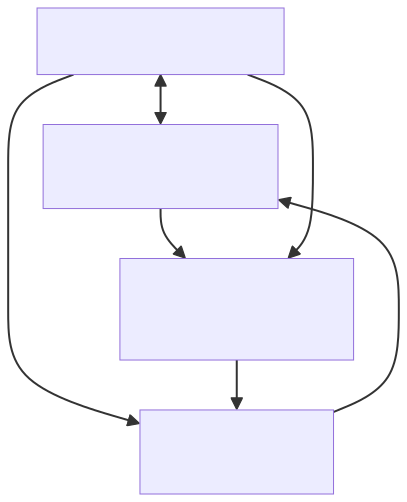
\includegraphics[width=0.6\textwidth,height=\textheight]{../shared-assets/trial-organisation-overview-figure.png}

}

\caption{\label{fig-organisation-overview}Trial organisation overview.}

\end{figure}

Trial management and oversight is governed by three trial committees and
groups: the Trial Team (TT), the Trial Management Group (TMG), the joint
Trial Steering and Data Monitoring Committee (SDMC). These groups and
their relationships are briefly described in
Figure~\ref{fig-organisation-overview}. Details about each committee and
group are available in their respective charter.

\hypertarget{trial-team}{%
\subsection{Trial team}\label{trial-team}}

\textbf{Responsibility}

To run the trial on a day-to-day basis, maintain trial databases,
randomise clusters, ensuring complete and correct data, preparing
reports for meetings (including those of the TMG and SDMC) and dealing
with research governance and, if appropriate, regulatory matters.

\textbf{Composition}

Includes the project manager, clinical research associates, principal
investigator and co-investigators as needed.

\textbf{Relationships}

Reports to the TMG and SDMC. Operationalises decisions made by the TMG.

\textbf{Meeting frequencies}

As often as needed, often weekly or bi-weekly.

\hypertarget{trial-management-group-tmg}{%
\subsection{Trial Management Group
(TMG)}\label{trial-management-group-tmg}}

\textbf{Responsibility}

To manage the trial, including its clinical and practical aspects.

\textbf{Composition}

Includes members with broad expertise appropriate to the trial. The TMG
will be chaired by the Principal Investigator.

\textbf{Relationships}

Receives reports from TT. Provides input to the SDMC. Implements
decisions made by the SDMC.

\textbf{Meeting frequencies}

Monthly to every six months.

\hypertarget{joint-trial-steering-and-data-monitoring-committee-sdmc}{%
\subsection{Joint Trial Steering and Data Monitoring Committee
(SDMC)}\label{joint-trial-steering-and-data-monitoring-committee-sdmc}}

\textbf{Responsibility}

The SDMC's responsibility is to oversee the trial, review results of
interim analyses and safety events reported by the TMG, and review trial
data for each batch, assessing data quality, completeness, cluster
performance in recruitment and loss to follow-up rates, and external
factors affecting trial validity, safety, or ethics. This committee also
offer guidance to the TMG.

\textbf{Composition}

A majority of independent members, including a chair and three
additional external experts specializing in the clinical area,
biostatistics, and a community or patient representative, as well as and
a minority of members with a direct interest in the trial, including the
principal investigator. The chair should be independent of the trial,
and the coordinating institutions Karolinska Institutet and The George
Institute for Global Health.

\textbf{Relationships}

Receives reports from the trial team and TMG.

\textbf{Meeting frequencies}

After the completion of each batch, but may be more frequent if needed.

\hypertarget{funding}{%
\section{Funding}\label{funding}}

\begin{itemize}
\tightlist
\item
  Swedish Research Council (reg. no. 2023-03128)
\item
  Laerdal Foundation (reg. no. 2023-0297)
\end{itemize}

\hypertarget{special-considerations}{%
\section{Special considerations}\label{special-considerations}}

\hypertarget{funding-1}{%
\subsection{Funding}\label{funding-1}}

This trial is not yet fully funded. The Trial Management Group has
decided to proceed with the trial with the expectation that additional
funding will be secured. The Trial Steering Committee will be informed
of the funding status at each meeting. If funding is not secured, the
trial will be stopped. This will likely result in an underpowered trial.
The justification for this decision is that the intervention is
considered standard of care in many countries and the data collection is
considered minimal risk. There is therefore a very small risk of harm to
patient participants, but a potential direct benefit to those patient
participants who receive the intervention. The benefit-risk ratio is
therefore considered to be favourable, even in the case of an
underpowered trial.

\hypertarget{potential-amendments}{%
\subsection{Potential amendments}\label{potential-amendments}}

There are ongoing discussions about re-framing the trial as a hybrid
effectiveness-implementation trial and include a cost-effectiveness
analysis. This would involve adding additional data collection to assess
the implementation and costs of the intervention. This would involve
additional funding and amended ethical approvals.

\hypertarget{notification-of-trial-completion-reporting-and-publication}{%
\section{Notification of trial completion, reporting, and
publication}\label{notification-of-trial-completion-reporting-and-publication}}

The trial will be reported to the Funders within a year of completion.
The results of the trial will also be prepared as manuscripts for
publication. Authorship on trial manuscripts will be based on the
International Committee of Medical Journal Editors (ICMJE)
criteria\textsuperscript{48}:

\begin{quote}
\begin{itemize}
\tightlist
\item
  Substantial contributions to the conception or design of the work; or
  the acquisition, analysis, or interpretation of data for the work; AND
\item
  Drafting the work or reviewing it critically for important
  intellectual content; AND
\item
  Final approval of the version to be published; AND
\item
  Agreement to be accountable for all aspects of the work in ensuring
  that questions related to the accuracy or integrity of any part of the
  work are appropriately investigated and resolved.
\end{itemize}

In addition to being accountable for the parts of the work done, an
author should be able to identify which co-authors are responsible for
specific other parts of the work. In addition, authors should have
confidence in the integrity of the contributions of their co-authors.
\end{quote}

The most recent version of the ICMJE criteria will be adhered to. We
will also use the ICMJE criteria for non-author contributorship.

Before work on a trial manuscript is initiated, a writing group will be
formed and first and last authors will be designated. This writing group
will be formed by discussion in the Trial Management Group.

\hypertarget{collection-handling-and-archiving-of-data}{%
\section{Collection, handling, and archiving of
data}\label{collection-handling-and-archiving-of-data}}

Clinical research coordinators will collect data using a paper based CRF
(see Appendix Section~\ref{sec-appendix-case-record-form}), which is
then transferred to an eCRF. All trial data in the CRF must be extracted
from and be consistent with the relevant source documents. The eCRF will
be accessible to trial coordinators, data managers, the Investigators,
Clinical Trial Monitors, Auditors, and Inspectors as required. All data
will be registered, managed, and stored in a manner that enables correct
reporting, interpretation, and verification. The complete Trial Master
File, as well as source documents, will be archived for at least 10
years after the trial is completed. Source data in the medical records
system are stored and archived in accordance with national regulations.
Metadata will be publicly accessible via a persistent DOI, and
anonymised data will be released upon project completion. A detailed
data management plan is available here
\url{https://doi.org/10.5281/zenodo.7748764}.

\hypertarget{source-data}{%
\subsection{Source data}\label{source-data}}

The source data for each variable is given in
Section~\ref{sec-variables}. Whenever medical records are the source
data, this includes imaging and lab reports. Whenever an interview is
given as the source, the CRF will constitute the source data, as this is
where the responses to questions will be recorded. The local
investigator must keep source documents for each patient participant in
the trial. A document describing what has been classified as source data
in the trial (source data reference document) will be included in the
Investigator Site File (ISF). The investigator must ensure that all
source documents are accessible for monitoring and other quality control
activities. Source data is further defined before trial start at each
individual site and can, in cases where source data is not registered in
another document, consist of the CRF. This should be decided in
consultation with the monitor and clearly stated in the source data
reference document. Access to trial-related documentation, such as
patient participants' medical records, CRFs, other source data and other
trial documentation will be provided for monitoring and auditing
purposes. Access will also be granted in the context of regulatory
inspections.

\hypertarget{sec-variables}{%
\subsection{Variables}\label{sec-variables}}

\hypertarget{screening-3}{%
\subsubsection{Screening}\label{screening-3}}

\begin{itemize}
\item
  \textbf{Screening ID}
\item
  \textbf{1. Date of screening}
\item
  \textbf{2. Date of data entry}
\item
  \textbf{1. Is the patient at least 15 years old?} Source: Medical
  record or interview

  \begin{enumerate}
  \def\labelenumi{\arabic{enumi}.}
  \tightlist
  \item
    Yes
  \item
    No
  \end{enumerate}
\item
  \textbf{2. Did the patient present with a history of trauma defined as
  having any of the reasons listed in the International Classification
  of Diseases chapter XX as the reason for presenting? Please see
  https://icd.who.int/browse10/2019/en\#/XX for a complete list of
  ICD-10 codes} Source: Medical record or interview

  \begin{enumerate}
  \def\labelenumi{\arabic{enumi}.}
  \tightlist
  \item
    Yes
  \item
    No
  \end{enumerate}
\item
  \textbf{3. Did the trauma occur less than 48 hours before arrival to
  the hospital?} Source: Medical record or interview

  \begin{enumerate}
  \def\labelenumi{\arabic{enumi}.}
  \tightlist
  \item
    Yes
  \item
    No
  \end{enumerate}
\item
  \textbf{4. Was the patient admitted?} Source: Medical record

  \begin{enumerate}
  \def\labelenumi{\arabic{enumi}.}
  \tightlist
  \item
    Yes
  \item
    No
  \end{enumerate}
\item
  \textbf{5. Did the patient die after arrival but before admission?}
  Source: Medical record

  \begin{enumerate}
  \def\labelenumi{\arabic{enumi}.}
  \tightlist
  \item
    Yes
  \item
    No
  \end{enumerate}
\item
  \textbf{6. Was the patient transferred to another hospital for
  admission?} Source: Medical record

  \begin{enumerate}
  \def\labelenumi{\arabic{enumi}.}
  \tightlist
  \item
    Yes
  \item
    No
  \end{enumerate}
\item
  \textbf{1. Did the patient present with isolated limb injury?} Source:
  Medical record

  \begin{enumerate}
  \def\labelenumi{\arabic{enumi}.}
  \tightlist
  \item
    Yes
  \item
    No
  \end{enumerate}
\item
  \textbf{2. Was the patient directly admitted to a ward without being
  seen by a physician in the emergency department?} Source: Medical
  record

  \begin{enumerate}
  \def\labelenumi{\arabic{enumi}.}
  \tightlist
  \item
    Yes
  \item
    No
  \end{enumerate}
\item
  \textbf{Is the patient eligible? (Eligible=1; Not Eligible=0)}
\item
  \textbf{Any other comments?}
\end{itemize}

\hypertarget{consent}{%
\subsubsection{Consent}\label{consent}}

\begin{itemize}
\item
  \textbf{1. Is this patient included under the waiver of informed
  consent because the patient is unconscious or otherwise unable to
  provide consent and do not have a legally acceptable representative?}

  \begin{enumerate}
  \def\labelenumi{\arabic{enumi}.}
  \tightlist
  \item
    Yes
  \item
    No
  \end{enumerate}
\item
  \textbf{1. Did the participant/ or legally acceptable representative
  (LAR) provided consent for collection of non-routinely recorded data}

  \begin{enumerate}
  \def\labelenumi{\arabic{enumi}.}
  \tightlist
  \item
    Yes
  \item
    No
  \end{enumerate}
\item
  \textbf{2. Who gave consent for collection of non-routinely recorded
  data?}

  \begin{enumerate}
  \def\labelenumi{\arabic{enumi}.}
  \tightlist
  \item
    Patient participant
  \item
    Legally acceptable representative
  \end{enumerate}
\item
  \textbf{3. What is the LAR's relationship with the participant?}
\item
  \textbf{4. Why was Legally acceptable representative (LAR) approached
  for consent for collection of non-routinely recorded data?}

  \begin{enumerate}
  \def\labelenumi{\arabic{enumi}.}
  \tightlist
  \item
    The participant is incapacitated because of the trauma
  \item
    The participant is younger than 18 years
  \end{enumerate}
\item
  \textbf{5. Date when participant or legally acceptable representative
  (LAR) gave consent for collection of non-routinely recorded data.}
\item
  \textbf{6. How did the participant or legally acceptable
  representative (LAR) consent for collection of non-routinely recorded
  data?}

  \begin{enumerate}
  \def\labelenumi{\arabic{enumi}.}
  \tightlist
  \item
    In writing
  \item
    Verbally
  \end{enumerate}
\item
  \textbf{7. Reconsenting done?}

  \begin{enumerate}
  \def\labelenumi{\arabic{enumi}.}
  \tightlist
  \item
    Yes
  \item
    No
  \end{enumerate}
\item
  \textbf{7.1 Date when the participant was reconsented?}
\item
  \textbf{7.2 Why consenting was not done?}
\item
  \textbf{1. Did the minor give assent for collection of non-routinely
  recorded data?}

  \begin{enumerate}
  \def\labelenumi{\arabic{enumi}.}
  \tightlist
  \item
    Yes
  \item
    No
  \end{enumerate}
\item
  \textbf{2. Date when the minor gave assent for collection of
  non-routinely recorded data.}
\item
  \textbf{3. In case the minor refused to participate, date when minor
  refused}
\item
  \textbf{1. Is the participant or LAR wants to opt out from study?}

  \begin{enumerate}
  \def\labelenumi{\arabic{enumi}.}
  \tightlist
  \item
    Yes
  \item
    No
  \end{enumerate}
\item
  \textbf{2. Who opted-out of the routinely recorded data
  (in-hospital)?}

  \begin{enumerate}
  \def\labelenumi{\arabic{enumi}.}
  \tightlist
  \item
    Patient participant
  \item
    Legally acceptable representative (LAR)
  \end{enumerate}
\item
  \textbf{3. Date when participant or legally acceptable representative
  (LAR) opted-out.}
\item
  \textbf{4. Did the participant or legally acceptable representative
  (LAR) suggested to delete all the previously recorded data?}

  \begin{enumerate}
  \def\labelenumi{\arabic{enumi}.}
  \tightlist
  \item
    Yes
  \item
    No
  \end{enumerate}
\item
  \textbf{Any other comments?}
\end{itemize}

\hypertarget{consent-withdrawn}{%
\subsubsection{Consent withdrawn}\label{consent-withdrawn}}

\begin{itemize}
\item
  \textbf{1. Does the participant or legally acceptable representative
  (LAR) want to withdraw the consent?}

  \begin{enumerate}
  \def\labelenumi{\arabic{enumi}.}
  \tightlist
  \item
    Yes
  \item
    No
  \end{enumerate}
\item
  \textbf{2. Date of consent withdrawal for follow-up data collection.}
\item
  \textbf{3. Procedure(s) for which consent has been withdrawn}

  \begin{enumerate}
  \def\labelenumi{\arabic{enumi}.}
  \tightlist
  \item
    Data collection prior to withdrawal
  \item
    All data collection after withdrawal
  \item
    Both
  \end{enumerate}
\item
  \textbf{Any other comments?}
\end{itemize}

\hypertarget{baseline}{%
\subsubsection{Baseline}\label{baseline}}

\begin{itemize}
\item
  \textbf{1. Age in years} Source: Medical record of interview
\item
  \textbf{2. Sex} Source: Medical record of interview

  \begin{enumerate}
  \def\labelenumi{\arabic{enumi}.}
  \tightlist
  \item
    Female
  \item
    Male
  \item
    Other
  \item
    Not known
  \end{enumerate}
\item
  \textbf{3. Current marital status} Requires opt-in consent, not
  routinely recorded. Source: Interview

  \begin{enumerate}
  \def\labelenumi{\arabic{enumi}.}
  \tightlist
  \item
    Never married
  \item
    Currently married
  \item
    Separated
  \item
    Divorced
  \item
    Widowed
  \item
    Cohabiting
  \item
    Not known
  \end{enumerate}
\item
  \textbf{4. Education level} Requires opt-in consent, not routinely
  recorded. Source: Interview

  \begin{enumerate}
  \def\labelenumi{\arabic{enumi}.}
  \tightlist
  \item
    Not attended school
  \item
    Primary school
  \item
    Secondary school
  \item
    Higher secondary school
  \item
    Graduate
  \item
    Post graduate and above
  \item
    Other
  \item
    Not known
  \end{enumerate}
\item
  \textbf{5. If other, please specify} Requires opt-in consent, not
  routinely recorded. Source: Interview
\item
  \textbf{6. Main work status} Requires opt-in consent, not routinely
  recorded. Source: Interview

  \begin{enumerate}
  \def\labelenumi{\arabic{enumi}.}
  \tightlist
  \item
    Paid work, such as daily wage earner, teacher, factory worker and
    government employee
  \item
    Self-employed, such as own your business or farming
  \item
    Non-paid work, such as volunteer or charity
  \item
    Student
  \item
    Keeping house/homemaker
  \item
    Retired
  \item
    Unemployed (health reasons)
  \item
    Unemployed (other reasons)
  \item
    Other
  \item
    No income
  \item
    Not known
  \end{enumerate}
\item
  \textbf{7. If other, please specify} Requires opt-in consent, not
  routinely recorded. Source: Interview
\item
  \textbf{8. Income level in INR per month} Requires opt-in consent, not
  routinely recorded. Source: Interview

  \begin{enumerate}
  \def\labelenumi{\arabic{enumi}.}
  \tightlist
  \item
    Below 10,000
  \item
    10,001-20,000
  \item
    20,001-30,000
  \item
    30,001-50,000
  \item
    50,001-80,000
  \item
    80,001-1,00,000
  \item
    Above 1,00,000
  \item
    No income
  \item
    Not known
  \end{enumerate}
\item
  \textbf{9. Mechanism of injury description}
\item
  \textbf{10. Mechanism of injury ICD 10 code} Coded using ICD 10.
  Please see https://icd.who.int/browse10/2019/en\#/XX for a complete
  list of ICD-10 codes. Source: Medical record

  \begin{enumerate}
  \def\labelenumi{\arabic{enumi}.}
  \setcounter{enumi}{1109}
  \tightlist
  \item
    V01 Pedestrian injured in collision with pedal cycle
  \item
    V01.0 Pedestrian injured in collision with pedal cycle : nontraffic
    accident
  \item
    V01.1 Pedestrian injured in collision with pedal cycle : traffic
    accident
  \item
    V01.9 Pedestrian injured in collision with pedal cycle : unspecified
    whether traffic or nontraffic accident
  \item
    V02 Pedestrian injured in collision with two- or three-wheeled motor
    vehicle
  \item
    V02.0 Pedestrian injured in collision with two- or three-wheeled
    motor vehicle : nontraffic accident
  \item
    V02.1 Pedestrian injured in collision with two- or three-wheeled
    motor vehicle : traffic accident
  \item
    V02.9 Pedestrian injured in collision with two- or three-wheeled
    motor vehicle : unspecified whether traffic or nontraffic accident
  \item
    V03 Pedestrian injured in collision with car, pick-up truck or van
  \item
    V03.0 Pedestrian injured in collision with car, pick-up truck or van
    : nontraffic accident
  \item
    V03.1 Pedestrian injured in collision with car, pick-up truck or van
    : traffic accident
  \item
    V03.9 Pedestrian injured in collision with car, pick-up truck or van
    : unspecified whether traffic or nontraffic accident
  \item
    V04 Pedestrian injured in collision with heavy transport vehicle or
    bus
  \item
    V04.0 Pedestrian injured in collision with heavy transport vehicle
    or bus : nontraffic accident
  \item
    V04.1 Pedestrian injured in collision with heavy transport vehicle
    or bus : traffic accident
  \item
    V04.9 Pedestrian injured in collision with heavy transport vehicle
    or bus : unspecified whether traffic or nontraffic accident
  \item
    V05 Pedestrian injured in collision with railway train or railway
    vehicle
  \item
    V05.0 Pedestrian injured in collision with railway train or railway
    vehicle : nontraffic accident
  \item
    V05.1 Pedestrian injured in collision with railway train or railway
    vehicle : traffic accident
  \item
    V05.9 Pedestrian injured in collision with railway train or railway
    vehicle : unspecified whether traffic or nontraffic accident
  \item
    V06 Pedestrian injured in collision with other nonmotor vehicle
  \item
    V06.0 Pedestrian injured in collision with other nonmotor vehicle :
    nontraffic accident
  \item
    V06.1 Pedestrian injured in collision with other nonmotor vehicle :
    traffic accident
  \item
    V06.9 Pedestrian injured in collision with other nonmotor vehicle :
    unspecified whether traffic or nontraffic accident
  \item
    V09 Pedestrian injured in other and unspecified transport accidents
  \item
    V09.0 Pedestrian injured in nontraffic accident involving other and
    unspecified motor vehicles
  \item
    V09.1 Pedestrian injured in unspecified nontraffic accident
  \item
    V09.2 Pedestrian injured in traffic accident involving other and
    unspecified motor vehicles
  \item
    V09.3 Pedestrian injured in unspecified traffic accident
  \item
    V09.9 Pedestrian injured in unspecified transport accident
  \item
    V10 Pedal cyclist injured in collision with pedestrian or animal
  \item
    V10.0 Pedal cyclist injured in collision with pedestrian or animal :
    driver injured in nontraffic accident
  \item
    V10.1 Pedal cyclist injured in collision with pedestrian or animal :
    passenger injured in nontraffic accident
  \item
    V10.2 Pedal cyclist injured in collision with pedestrian or animal :
    unspecified pedal cyclist injured in nontraffic accident
  \item
    V10.3 Pedal cyclist injured in collision with pedestrian or animal :
    person injured while boarding or alighting
  \item
    V10.4 Pedal cyclist injured in collision with pedestrian or animal :
    driver injured in traffic accident
  \item
    V10.5 Pedal cyclist injured in collision with pedestrian or animal :
    passenger injured in traffic accident
  \item
    V10.9 Pedal cyclist injured in collision with pedestrian or animal :
    unspecified pedal cyclist injured in traffic accident
  \item
    V11 Pedal cyclist injured in collision with other pedal cycle
  \item
    V11.0 Pedal cyclist injured in collision with other pedal cycle :
    driver injured in nontraffic accident
  \item
    V11.1 Pedal cyclist injured in collision with other pedal cycle :
    passenger injured in nontraffic accident
  \item
    V11.2 Pedal cyclist injured in collision with other pedal cycle :
    unspecified pedal cyclist injured in nontraffic accident
  \item
    V11.3 Pedal cyclist injured in collision with other pedal cycle :
    person injured while boarding or alighting
  \item
    V11.4 Pedal cyclist injured in collision with other pedal cycle :
    driver injured in traffic accident
  \item
    V11.5 Pedal cyclist injured in collision with other pedal cycle :
    passenger injured in traffic accident
  \item
    V11.9 Pedal cyclist injured in collision with other pedal cycle :
    unspecified pedal cyclist injured in traffic accident
  \item
    V12 Pedal cyclist injured in collision with two- or three-wheeled
    motor vehicle
  \item
    V12.0 Pedal cyclist injured in collision with two- or three-wheeled
    motor vehicle : driver injured in nontraffic accident
  \item
    V12.1 Pedal cyclist injured in collision with two- or three-wheeled
    motor vehicle : passenger injured in nontraffic accident
  \item
    V12.2 Pedal cyclist injured in collision with two- or three-wheeled
    motor vehicle : unspecified pedal cyclist injured in nontraffic
    accident
  \item
    V12.3 Pedal cyclist injured in collision with two- or three-wheeled
    motor vehicle : person injured while boarding or alighting
  \item
    V12.4 Pedal cyclist injured in collision with two- or three-wheeled
    motor vehicle : driver injured in traffic accident
  \item
    V12.5 Pedal cyclist injured in collision with two- or three-wheeled
    motor vehicle : passenger injured in traffic accident
  \item
    V12.9 Pedal cyclist injured in collision with two- or three-wheeled
    motor vehicle : unspecified pedal cyclist injured in traffic
    accident
  \item
    V13 Pedal cyclist injured in collision with car, pick-up truck or
    van
  \item
    V13.0 Pedal cyclist injured in collision with car, pick-up truck or
    van : driver injured in nontraffic accident
  \item
    V13.1 Pedal cyclist injured in collision with car, pick-up truck or
    van : passenger injured in nontraffic accident
  \item
    V13.2 Pedal cyclist injured in collision with car, pick-up truck or
    van : unspecified pedal cyclist injured in nontraffic accident
  \item
    V13.3 Pedal cyclist injured in collision with car, pick-up truck or
    van : person injured while boarding or alighting
  \item
    V13.4 Pedal cyclist injured in collision with car, pick-up truck or
    van : driver injured in traffic accident
  \item
    V13.5 Pedal cyclist injured in collision with car, pick-up truck or
    van : passenger injured in traffic accident
  \item
    V13.9 Pedal cyclist injured in collision with car, pick-up truck or
    van : unspecified pedal cyclist injured in traffic accident
  \item
    V14 Pedal cyclist injured in collision with heavy transport vehicle
    or bus
  \item
    V14.0 Pedal cyclist injured in collision with heavy transport
    vehicle or bus : driver injured in nontraffic accident
  \item
    V14.1 Pedal cyclist injured in collision with heavy transport
    vehicle or bus : passenger injured in nontraffic accident
  \item
    V14.2 Pedal cyclist injured in collision with heavy transport
    vehicle or bus : unspecified pedal cyclist injured in nontraffic
    accident
  \item
    V14.3 Pedal cyclist injured in collision with heavy transport
    vehicle or bus : person injured while boarding or alighting
  \item
    V14.4 Pedal cyclist injured in collision with heavy transport
    vehicle or bus : driver injured in traffic accident
  \item
    V14.5 Pedal cyclist injured in collision with heavy transport
    vehicle or bus : passenger injured in traffic accident
  \item
    V14.9 Pedal cyclist injured in collision with heavy transport
    vehicle or bus : unspecified pedal cyclist injured in traffic
    accident
  \item
    V15 Pedal cyclist injured in collision with railway train or railway
    vehicle
  \item
    V15.0 Pedal cyclist injured in collision with railway train or
    railway vehicle : driver injured in nontraffic accident
  \item
    V15.1 Pedal cyclist injured in collision with railway train or
    railway vehicle : passenger injured in nontraffic accident
  \item
    V15.2 Pedal cyclist injured in collision with railway train or
    railway vehicle : unspecified pedal cyclist injured in nontraffic
    accident
  \item
    V15.3 Pedal cyclist injured in collision with railway train or
    railway vehicle : person injured while boarding or alighting
  \item
    V15.4 Pedal cyclist injured in collision with railway train or
    railway vehicle : driver injured in traffic accident
  \item
    V15.5 Pedal cyclist injured in collision with railway train or
    railway vehicle : passenger injured in traffic accident
  \item
    V15.9 Pedal cyclist injured in collision with railway train or
    railway vehicle : unspecified pedal cyclist injured in traffic
    accident
  \item
    V16 Pedal cyclist injured in collision with other nonmotor vehicle
  \item
    V16.0 Pedal cyclist injured in collision with other nonmotor vehicle
    : driver injured in nontraffic accident
  \item
    V16.1 Pedal cyclist injured in collision with other nonmotor vehicle
    : passenger injured in nontraffic accident
  \item
    V16.2 Pedal cyclist injured in collision with other nonmotor vehicle
    : unspecified pedal cyclist injured in nontraffic accident
  \item
    V16.3 Pedal cyclist injured in collision with other nonmotor vehicle
    : person injured while boarding or alighting
  \item
    V16.4 Pedal cyclist injured in collision with other nonmotor vehicle
    : driver injured in traffic accident
  \item
    V16.5 Pedal cyclist injured in collision with other nonmotor vehicle
    : passenger injured in traffic accident
  \item
    V16.9 Pedal cyclist injured in collision with other nonmotor vehicle
    : unspecified pedal cyclist injured in traffic accident
  \item
    V17 Pedal cyclist injured in collision with fixed or stationary
    object
  \item
    V17.0 Pedal cyclist injured in collision with fixed or stationary
    object : driver injured in nontraffic accident
  \item
    V17.1 Pedal cyclist injured in collision with fixed or stationary
    object : passenger injured in nontraffic accident
  \item
    V17.2 Pedal cyclist injured in collision with fixed or stationary
    object : unspecified pedal cyclist injured in nontraffic accident
  \item
    V17.3 Pedal cyclist injured in collision with fixed or stationary
    object : person injured while boarding or alighting
  \item
    V17.4 Pedal cyclist injured in collision with fixed or stationary
    object : driver injured in traffic accident
  \item
    V17.5 Pedal cyclist injured in collision with fixed or stationary
    object : passenger injured in traffic accident
  \item
    V17.9 Pedal cyclist injured in collision with fixed or stationary
    object : unspecified pedal cyclist injured in traffic accident
  \item
    V18 Pedal cyclist injured in noncollision transport accident
  \item
    V18.0 Pedal cyclist injured in noncollision transport accident :
    driver injured in nontraffic accident
  \item
    V18.1 Pedal cyclist injured in noncollision transport accident :
    passenger injured in nontraffic accident
  \item
    V18.2 Pedal cyclist injured in noncollision transport accident :
    unspecified pedal cyclist injured in nontraffic accident
  \item
    V18.3 Pedal cyclist injured in noncollision transport accident :
    person injured while boarding or alighting
  \item
    V18.4 Pedal cyclist injured in noncollision transport accident :
    driver injured in traffic accident
  \item
    V18.5 Pedal cyclist injured in noncollision transport accident :
    passenger injured in traffic accident
  \item
    V18.9 Pedal cyclist injured in noncollision transport accident :
    unspecified pedal cyclist injured in traffic accident
  \item
    V19 Pedal cyclist injured in other and unspecified transport
    accidents
  \item
    V19.0 Driver injured in collision with other and unspecified motor
    vehicles in nontraffic accident
  \item
    V19.1 Passenger injured in collision with other and unspecified
    motor vehicles in nontraffic accident
  \item
    V19.2 Unspecified pedal cyclist injured in collision with other and
    unspecified motor vehicles in nontraffic accident
  \item
    V19.3 Pedal cyclist {[}any{]} injured in unspecified nontraffic
    accident
  \item
    V19.4 Driver injured in collision with other and unspecified motor
    vehicles in traffic accident
  \item
    V19.5 Passenger injured in collision with other and unspecified
    motor vehicles in traffic accident
  \item
    V19.6 Unspecified pedal cyclist injured in collision with other and
    unspecified motor vehicles in traffic accident
  \item
    V19.8 Pedal cyclist {[}any{]} injured in other specified transport
    accidents
  \item
    V19.9 Pedal cyclist {[}any{]} injured in unspecified traffic
    accident
  \item
    V20 Motorcycle rider injured in collision with pedestrian or animal
  \item
    V20.0 Motorcycle rider injured in collision with pedestrian or
    animal : driver injured in nontraffic accident
  \item
    V20.1 Motorcycle rider injured in collision with pedestrian or
    animal : passenger injured in nontraffic accident
  \item
    V20.2 Motorcycle rider injured in collision with pedestrian or
    animal : unspecified motorcycle rider injured in nontraffic accident
  \item
    V20.3 Motorcycle rider injured in collision with pedestrian or
    animal : person injured while boarding or alighting
  \item
    V20.4 Motorcycle rider injured in collision with pedestrian or
    animal : driver injured in traffic accident
  \item
    V20.5 Motorcycle rider injured in collision with pedestrian or
    animal : passenger injured in traffic accident
  \item
    V20.9 Motorcycle rider injured in collision with pedestrian or
    animal : unspecified motorcycle rider injured in traffic accident
  \item
    V21 Motorcycle rider injured in collision with pedal cycle
  \item
    V21.0 Motorcycle rider injured in collision with pedal cycle :
    driver injured in nontraffic accident
  \item
    V21.1 Motorcycle rider injured in collision with pedal cycle :
    passenger injured in nontraffic accident
  \item
    V21.2 Motorcycle rider injured in collision with pedal cycle :
    unspecified motorcycle rider injured in nontraffic accident
  \item
    V21.3 Motorcycle rider injured in collision with pedal cycle :
    person injured while boarding or alighting
  \item
    V21.4 Motorcycle rider injured in collision with pedal cycle :
    driver injured in traffic accident
  \item
    V21.5 Motorcycle rider injured in collision with pedal cycle :
    passenger injured in traffic accident
  \item
    V21.9 Motorcycle rider injured in collision with pedal cycle :
    unspecified motorcycle rider injured in traffic accident
  \item
    V22 Motorcycle rider injured in collision with two- or three-wheeled
    motor vehicle
  \item
    V22.0 Motorcycle rider injured in collision with two- or
    three-wheeled motor vehicle : driver injured in nontraffic accident
  \item
    V22.1 Motorcycle rider injured in collision with two- or
    three-wheeled motor vehicle : passenger injured in nontraffic
    accident
  \item
    V22.2 Motorcycle rider injured in collision with two- or
    three-wheeled motor vehicle : unspecified motorcycle rider injured
    in nontraffic accident
  \item
    V22.3 Motorcycle rider injured in collision with two- or
    three-wheeled motor vehicle : person injured while boarding or
    alighting
  \item
    V22.4 Motorcycle rider injured in collision with two- or
    three-wheeled motor vehicle : driver injured in traffic accident
  \item
    V22.5 Motorcycle rider injured in collision with two- or
    three-wheeled motor vehicle : passenger injured in traffic accident
  \item
    V22.9 Motorcycle rider injured in collision with two- or
    three-wheeled motor vehicle : unspecified motorcycle rider injured
    in traffic accident
  \item
    V23 Motorcycle rider injured in collision with car, pick-up truck or
    van
  \item
    V23.0 Motorcycle rider injured in collision with car, pick-up truck
    or van : driver injured in nontraffic accident
  \item
    V23.1 Motorcycle rider injured in collision with car, pick-up truck
    or van : passenger injured in nontraffic accident
  \item
    V23.2 Motorcycle rider injured in collision with car, pick-up truck
    or van : unspecified motorcycle rider injured in nontraffic accident
  \item
    V23.3 Motorcycle rider injured in collision with car, pick-up truck
    or van : person injured while boarding or alighting
  \item
    V23.4 Motorcycle rider injured in collision with car, pick-up truck
    or van : driver injured in traffic accident
  \item
    V23.5 Motorcycle rider injured in collision with car, pick-up truck
    or van : passenger injured in traffic accident
  \item
    V23.9 Motorcycle rider injured in collision with car, pick-up truck
    or van : unspecified motorcycle rider injured in traffic accident
  \item
    V24 Motorcycle rider injured in collision with heavy transport
    vehicle or bus
  \item
    V24.0 Motorcycle rider injured in collision with heavy transport
    vehicle or bus : driver injured in nontraffic accident
  \item
    V24.1 Motorcycle rider injured in collision with heavy transport
    vehicle or bus : passenger injured in nontraffic accident
  \item
    V24.2 Motorcycle rider injured in collision with heavy transport
    vehicle or bus : unspecified motorcycle rider injured in nontraffic
    accident
  \item
    V24.3 Motorcycle rider injured in collision with heavy transport
    vehicle or bus : person injured while boarding or alighting
  \item
    V24.4 Motorcycle rider injured in collision with heavy transport
    vehicle or bus : driver injured in traffic accident
  \item
    V24.5 Motorcycle rider injured in collision with heavy transport
    vehicle or bus : passenger injured in traffic accident
  \item
    V24.9 Motorcycle rider injured in collision with heavy transport
    vehicle or bus : unspecified motorcycle rider injured in traffic
    accident
  \item
    V25 Motorcycle rider injured in collision with railway train or
    railway vehicle
  \item
    V25.0 Motorcycle rider injured in collision with railway train or
    railway vehicle : driver injured in nontraffic accident
  \item
    V25.1 Motorcycle rider injured in collision with railway train or
    railway vehicle : passenger injured in nontraffic accident
  \item
    V25.2 Motorcycle rider injured in collision with railway train or
    railway vehicle : unspecified motorcycle rider injured in nontraffic
    accident
  \item
    V25.3 Motorcycle rider injured in collision with railway train or
    railway vehicle : person injured while boarding or alighting
  \item
    V25.4 Motorcycle rider injured in collision with railway train or
    railway vehicle : driver injured in traffic accident
  \item
    V25.5 Motorcycle rider injured in collision with railway train or
    railway vehicle : passenger injured in traffic accident
  \item
    V25.9 Motorcycle rider injured in collision with railway train or
    railway vehicle : unspecified motorcycle rider injured in traffic
    accident
  \item
    V26 Motorcycle rider injured in collision with other nonmotor
    vehicle
  \item
    V26.0 Motorcycle rider injured in collision with other nonmotor
    vehicle : driver injured in nontraffic accident
  \item
    V26.1 Motorcycle rider injured in collision with other nonmotor
    vehicle : passenger injured in nontraffic accident
  \item
    V26.2 Motorcycle rider injured in collision with other nonmotor
    vehicle : unspecified motorcycle rider injured in nontraffic
    accident
  \item
    V26.3 Motorcycle rider injured in collision with other nonmotor
    vehicle : person injured while boarding or alighting
  \item
    V26.4 Motorcycle rider injured in collision with other nonmotor
    vehicle : driver injured in traffic accident
  \item
    V26.5 Motorcycle rider injured in collision with other nonmotor
    vehicle : passenger injured in traffic accident
  \item
    V26.9 Motorcycle rider injured in collision with other nonmotor
    vehicle : unspecified motorcycle rider injured in traffic accident
  \item
    V27 Motorcycle rider injured in collision with fixed or stationary
    object
  \item
    V27.0 Motorcycle rider injured in collision with fixed or stationary
    object : driver injured in nontraffic accident
  \item
    V27.1 Motorcycle rider injured in collision with fixed or stationary
    object : passenger injured in nontraffic accident
  \item
    V27.2 Motorcycle rider injured in collision with fixed or stationary
    object : unspecified motorcycle rider injured in nontraffic accident
  \item
    V27.3 Motorcycle rider injured in collision with fixed or stationary
    object : person injured while boarding or alighting
  \item
    V27.4 Motorcycle rider injured in collision with fixed or stationary
    object : driver injured in traffic accident
  \item
    V27.5 Motorcycle rider injured in collision with fixed or stationary
    object : passenger injured in traffic accident
  \item
    V27.9 Motorcycle rider injured in collision with fixed or stationary
    object : unspecified motorcycle rider injured in traffic accident
  \item
    V28 Motorcycle rider injured in noncollision transport accident
  \item
    V28.0 Motorcycle rider injured in noncollision transport accident :
    driver injured in nontraffic accident
  \item
    V28.1 Motorcycle rider injured in noncollision transport accident :
    passenger injured in nontraffic accident
  \item
    V28.2 Motorcycle rider injured in noncollision transport accident :
    unspecified motorcycle rider injured in nontraffic accident
  \item
    V28.3 Motorcycle rider injured in noncollision transport accident :
    person injured while boarding or alighting
  \item
    V28.4 Motorcycle rider injured in noncollision transport accident :
    driver injured in traffic accident
  \item
    V28.5 Motorcycle rider injured in noncollision transport accident :
    passenger injured in traffic accident
  \item
    V28.9 Motorcycle rider injured in noncollision transport accident :
    unspecified motorcycle rider injured in traffic accident
  \item
    V29 Motorcycle rider injured in other and unspecified transport
    accidents
  \item
    V29.0 Driver injured in collision with other and unspecified motor
    vehicles in nontraffic accident
  \item
    V29.1 Passenger injured in collision with other and unspecified
    motor vehicles in nontraffic accident
  \item
    V29.2 Unspecified motorcycle rider injured in collision with other
    and unspecified motor vehicles in nontraffic accident
  \item
    V29.3 Motorcycle rider {[}any{]} injured in unspecified nontraffic
    accident
  \item
    V29.4 Driver injured in collision with other and unspecified motor
    vehicles in traffic accident
  \item
    V29.5 Passenger injured in collision with other and unspecified
    motor vehicles in traffic accident
  \item
    V29.6 Unspecified motorcycle rider injured in collision with other
    and unspecified motor vehicles in traffic accident
  \item
    V29.8 Motorcycle rider {[}any{]} injured in other specified
    transport accidents
  \item
    V29.9 Motorcycle rider {[}any{]} injured in unspecified traffic
    accident
  \item
    V30 Occupant of three-wheeled motor vehicle injured in collision
    with pedestrian or animal
  \item
    V30.0 Occupant of three-wheeled motor vehicle injured in collision
    with pedestrian or animal : driver injured in nontraffic accident
  \item
    V30.1 Occupant of three-wheeled motor vehicle injured in collision
    with pedestrian or animal : passenger injured in nontraffic accident
  \item
    V30.2 Occupant of three-wheeled motor vehicle injured in collision
    with pedestrian or animal : person on outside of vehicle injured in
    nontraffic accident
  \item
    V30.3 Occupant of three-wheeled motor vehicle injured in collision
    with pedestrian or animal : unspecified occupant of three-wheeled
    motor vehicle injured in nontraffic accident
  \item
    V30.4 Occupant of three-wheeled motor vehicle injured in collision
    with pedestrian or animal : person injured while boarding or
    alighting
  \item
    V30.5 Occupant of three-wheeled motor vehicle injured in collision
    with pedestrian or animal : driver injured in traffic accident
  \item
    V30.6 Occupant of three-wheeled motor vehicle injured in collision
    with pedestrian or animal : passenger injured in traffic accident
  \item
    V30.7 Occupant of three-wheeled motor vehicle injured in collision
    with pedestrian or animal : person on outside of vehicle injured in
    traffic accident
  \item
    V30.9 Occupant of three-wheeled motor vehicle injured in collision
    with pedestrian or animal : unspecified occupant of three-wheeled
    motor vehicle injured in traffic accident
  \item
    V31 Occupant of three-wheeled motor vehicle injured in collision
    with pedal cycle
  \item
    V31.0 Occupant of three-wheeled motor vehicle injured in collision
    with pedal cycle : driver injured in nontraffic accident
  \item
    V31.1 Occupant of three-wheeled motor vehicle injured in collision
    with pedal cycle : passenger injured in nontraffic accident
  \item
    V31.2 Occupant of three-wheeled motor vehicle injured in collision
    with pedal cycle : person on outside of vehicle injured in
    nontraffic accident
  \item
    V31.3 Occupant of three-wheeled motor vehicle injured in collision
    with pedal cycle : unspecified occupant of three-wheeled motor
    vehicle injured in nontraffic accident
  \item
    V31.4 Occupant of three-wheeled motor vehicle injured in collision
    with pedal cycle : person injured while boarding or alighting
  \item
    V31.5 Occupant of three-wheeled motor vehicle injured in collision
    with pedal cycle : driver injured in traffic accident
  \item
    V31.6 Occupant of three-wheeled motor vehicle injured in collision
    with pedal cycle : passenger injured in traffic accident
  \item
    V31.7 Occupant of three-wheeled motor vehicle injured in collision
    with pedal cycle : person on outside of vehicle injured in traffic
    accident
  \item
    V31.9 Occupant of three-wheeled motor vehicle injured in collision
    with pedal cycle : unspecified occupant of three-wheeled motor
    vehicle injured in traffic accident
  \item
    V32 Occupant of three-wheeled motor vehicle injured in collision
    with two- or three-wheeled motor vehicle
  \item
    V32.0 Occupant of three-wheeled motor vehicle injured in collision
    with two- or three-wheeled motor vehicle : driver injured in
    nontraffic accident
  \item
    V32.1 Occupant of three-wheeled motor vehicle injured in collision
    with two- or three-wheeled motor vehicle : passenger injured in
    nontraffic accident
  \item
    V32.2 Occupant of three-wheeled motor vehicle injured in collision
    with two- or three-wheeled motor vehicle : person on outside of
    vehicle injured in nontraffic accident
  \item
    V32.3 Occupant of three-wheeled motor vehicle injured in collision
    with two- or three-wheeled motor vehicle : unspecified occupant of
    three-wheeled motor vehicle injured in nontraffic accident
  \item
    V32.4 Occupant of three-wheeled motor vehicle injured in collision
    with two- or three-wheeled motor vehicle : person injured while
    boarding or alighting
  \item
    V32.5 Occupant of three-wheeled motor vehicle injured in collision
    with two- or three-wheeled motor vehicle : driver injured in traffic
    accident
  \item
    V32.6 Occupant of three-wheeled motor vehicle injured in collision
    with two- or three-wheeled motor vehicle : passenger injured in
    traffic accident
  \item
    V32.7 Occupant of three-wheeled motor vehicle injured in collision
    with two- or three-wheeled motor vehicle : person on outside of
    vehicle injured in traffic accident
  \item
    V32.9 Occupant of three-wheeled motor vehicle injured in collision
    with two- or three-wheeled motor vehicle : unspecified occupant of
    three-wheeled motor vehicle injured in traffic accident
  \item
    V33 Occupant of three-wheeled motor vehicle injured in collision
    with car, pick-up truck or van
  \item
    V33.0 Occupant of three-wheeled motor vehicle injured in collision
    with car, pick-up truck or van : driver injured in nontraffic
    accident
  \item
    V33.1 Occupant of three-wheeled motor vehicle injured in collision
    with car, pick-up truck or van : passenger injured in nontraffic
    accident
  \item
    V33.2 Occupant of three-wheeled motor vehicle injured in collision
    with car, pick-up truck or van : person on outside of vehicle
    injured in nontraffic accident
  \item
    V33.3 Occupant of three-wheeled motor vehicle injured in collision
    with car, pick-up truck or van : unspecified occupant of
    three-wheeled motor vehicle injured in nontraffic accident
  \item
    V33.4 Occupant of three-wheeled motor vehicle injured in collision
    with car, pick-up truck or van : person injured while boarding or
    alighting
  \item
    V33.5 Occupant of three-wheeled motor vehicle injured in collision
    with car, pick-up truck or van : driver injured in traffic accident
  \item
    V33.6 Occupant of three-wheeled motor vehicle injured in collision
    with car, pick-up truck or van : passenger injured in traffic
    accident
  \item
    V33.7 Occupant of three-wheeled motor vehicle injured in collision
    with car, pick-up truck or van : person on outside of vehicle
    injured in traffic accident
  \item
    V33.9 Occupant of three-wheeled motor vehicle injured in collision
    with car, pick-up truck or van : unspecified occupant of
    three-wheeled motor vehicle injured in traffic accident
  \item
    V34 Occupant of three-wheeled motor vehicle injured in collision
    with heavy transport vehicle or bus
  \item
    V34.0 Occupant of three-wheeled motor vehicle injured in collision
    with heavy transport vehicle or bus : driver injured in nontraffic
    accident
  \item
    V34.1 Occupant of three-wheeled motor vehicle injured in collision
    with heavy transport vehicle or bus : passenger injured in
    nontraffic accident
  \item
    V34.2 Occupant of three-wheeled motor vehicle injured in collision
    with heavy transport vehicle or bus : person on outside of vehicle
    injured in nontraffic accident
  \item
    V34.3 Occupant of three-wheeled motor vehicle injured in collision
    with heavy transport vehicle or bus : unspecified occupant of
    three-wheeled motor vehicle injured in nontraffic accident
  \item
    V34.4 Occupant of three-wheeled motor vehicle injured in collision
    with heavy transport vehicle or bus : person injured while boarding
    or alighting
  \item
    V34.5 Occupant of three-wheeled motor vehicle injured in collision
    with heavy transport vehicle or bus : driver injured in traffic
    accident
  \item
    V34.6 Occupant of three-wheeled motor vehicle injured in collision
    with heavy transport vehicle or bus : passenger injured in traffic
    accident
  \item
    V34.7 Occupant of three-wheeled motor vehicle injured in collision
    with heavy transport vehicle or bus : person on outside of vehicle
    injured in traffic accident
  \item
    V34.9 Occupant of three-wheeled motor vehicle injured in collision
    with heavy transport vehicle or bus : unspecified occupant of
    three-wheeled motor vehicle injured in traffic accident
  \item
    V35 Occupant of three-wheeled motor vehicle injured in collision
    with railway train or railway vehicle
  \item
    V35.0 Occupant of three-wheeled motor vehicle injured in collision
    with railway train or railway vehicle : driver injured in nontraffic
    accident
  \item
    V35.1 Occupant of three-wheeled motor vehicle injured in collision
    with railway train or railway vehicle : passenger injured in
    nontraffic accident
  \item
    V35.2 Occupant of three-wheeled motor vehicle injured in collision
    with railway train or railway vehicle : person on outside of vehicle
    injured in nontraffic accident
  \item
    V35.3 Occupant of three-wheeled motor vehicle injured in collision
    with railway train or railway vehicle : unspecified occupant of
    three-wheeled motor vehicle injured in nontraffic accident
  \item
    V35.4 Occupant of three-wheeled motor vehicle injured in collision
    with railway train or railway vehicle : person injured while
    boarding or alighting
  \item
    V35.5 Occupant of three-wheeled motor vehicle injured in collision
    with railway train or railway vehicle : driver injured in traffic
    accident
  \item
    V35.6 Occupant of three-wheeled motor vehicle injured in collision
    with railway train or railway vehicle : passenger injured in traffic
    accident
  \item
    V35.7 Occupant of three-wheeled motor vehicle injured in collision
    with railway train or railway vehicle : person on outside of vehicle
    injured in traffic accident
  \item
    V35.9 Occupant of three-wheeled motor vehicle injured in collision
    with railway train or railway vehicle : unspecified occupant of
    three-wheeled motor vehicle injured in traffic accident
  \item
    V36 Occupant of three-wheeled motor vehicle injured in collision
    with other nonmotor vehicle
  \item
    V36.0 Occupant of three-wheeled motor vehicle injured in collision
    with other nonmotor vehicle : driver injured in nontraffic accident
  \item
    V36.1 Occupant of three-wheeled motor vehicle injured in collision
    with other nonmotor vehicle : passenger injured in nontraffic
    accident
  \item
    V36.2 Occupant of three-wheeled motor vehicle injured in collision
    with other nonmotor vehicle : person on outside of vehicle injured
    in nontraffic accident
  \item
    V36.3 Occupant of three-wheeled motor vehicle injured in collision
    with other nonmotor vehicle : unspecified occupant of three-wheeled
    motor vehicle injured in nontraffic accident
  \item
    V36.4 Occupant of three-wheeled motor vehicle injured in collision
    with other nonmotor vehicle : person injured while boarding or
    alighting
  \item
    V36.5 Occupant of three-wheeled motor vehicle injured in collision
    with other nonmotor vehicle : driver injured in traffic accident
  \item
    V36.6 Occupant of three-wheeled motor vehicle injured in collision
    with other nonmotor vehicle : passenger injured in traffic accident
  \item
    V36.7 Occupant of three-wheeled motor vehicle injured in collision
    with other nonmotor vehicle : person on outside of vehicle injured
    in traffic accident
  \item
    V36.9 Occupant of three-wheeled motor vehicle injured in collision
    with other nonmotor vehicle : unspecified occupant of three-wheeled
    motor vehicle injured in traffic accident
  \item
    V37 Occupant of three-wheeled motor vehicle injured in collision
    with fixed or stationary object
  \item
    V37.0 Occupant of three-wheeled motor vehicle injured in collision
    with fixed or stationary object : driver injured in nontraffic
    accident
  \item
    V37.1 Occupant of three-wheeled motor vehicle injured in collision
    with fixed or stationary object : passenger injured in nontraffic
    accident
  \item
    V37.2 Occupant of three-wheeled motor vehicle injured in collision
    with fixed or stationary object : person on outside of vehicle
    injured in nontraffic accident
  \item
    V37.3 Occupant of three-wheeled motor vehicle injured in collision
    with fixed or stationary object : unspecified occupant of
    three-wheeled motor vehicle injured in nontraffic accident
  \item
    V37.4 Occupant of three-wheeled motor vehicle injured in collision
    with fixed or stationary object : person injured while boarding or
    alighting
  \item
    V37.5 Occupant of three-wheeled motor vehicle injured in collision
    with fixed or stationary object : driver injured in traffic accident
  \item
    V37.6 Occupant of three-wheeled motor vehicle injured in collision
    with fixed or stationary object : passenger injured in traffic
    accident
  \item
    V37.7 Occupant of three-wheeled motor vehicle injured in collision
    with fixed or stationary object : person on outside of vehicle
    injured in traffic accident
  \item
    V37.9 Occupant of three-wheeled motor vehicle injured in collision
    with fixed or stationary object : unspecified occupant of
    three-wheeled motor vehicle injured in traffic accident
  \item
    V38 Occupant of three-wheeled motor vehicle injured in noncollision
    transport accident
  \item
    V38.0 Occupant of three-wheeled motor vehicle injured in
    noncollision transport accident : driver injured in nontraffic
    accident
  \item
    V38.1 Occupant of three-wheeled motor vehicle injured in
    noncollision transport accident : passenger injured in nontraffic
    accident
  \item
    V38.2 Occupant of three-wheeled motor vehicle injured in
    noncollision transport accident : person on outside of vehicle
    injured in nontraffic accident
  \item
    V38.3 Occupant of three-wheeled motor vehicle injured in
    noncollision transport accident : unspecified occupant of
    three-wheeled motor vehicle injured in nontraffic accident
  \item
    V38.4 Occupant of three-wheeled motor vehicle injured in
    noncollision transport accident : person injured while boarding or
    alighting
  \item
    V38.5 Occupant of three-wheeled motor vehicle injured in
    noncollision transport accident : driver injured in traffic accident
  \item
    V38.6 Occupant of three-wheeled motor vehicle injured in
    noncollision transport accident : passenger injured in traffic
    accident
  \item
    V38.7 Occupant of three-wheeled motor vehicle injured in
    noncollision transport accident : person on outside of vehicle
    injured in traffic accident
  \item
    V38.9 Occupant of three-wheeled motor vehicle injured in
    noncollision transport accident : unspecified occupant of
    three-wheeled motor vehicle injured in traffic accident
  \item
    V39 Occupant of three-wheeled motor vehicle injured in other and
    unspecified transport accidents
  \item
    V39.0 Driver injured in collision with other and unspecified motor
    vehicles in nontraffic accident
  \item
    V39.1 Passenger injured in collision with other and unspecified
    motor vehicles in nontraffic accident
  \item
    V39.2 Unspecified occupant of three-wheeled motor vehicle injured in
    collision with other and unspecified motor vehicles in nontraffic
    accident
  \item
    V39.3 Occupant {[}any{]} of three-wheeled motor vehicle injured in
    unspecified nontraffic accident
  \item
    V39.4 Driver injured in collision with other and unspecified motor
    vehicles in traffic accident
  \item
    V39.5 Passenger injured in collision with other and unspecified
    motor vehicles in traffic accident
  \item
    V39.6 Unspecified occupant of three-wheeled motor vehicle injured in
    collision with other and unspecified motor vehicles in traffic
    accident
  \item
    V39.8 Occupant {[}any{]} of three-wheeled motor vehicle injured in
    other specified transport accidents
  \item
    V39.9 Occupant {[}any{]} of three-wheeled motor vehicle injured in
    unspecified traffic accident
  \item
    V40 Car occupant injured in collision with pedestrian or animal
  \item
    V40.0 Car occupant injured in collision with pedestrian or animal :
    driver injured in nontraffic accident
  \item
    V40.1 Car occupant injured in collision with pedestrian or animal :
    passenger injured in nontraffic accident
  \item
    V40.2 Car occupant injured in collision with pedestrian or animal :
    person on outside of vehicle injured in nontraffic accident
  \item
    V40.3 Car occupant injured in collision with pedestrian or animal :
    unspecified car occupant injured in nontraffic accident
  \item
    V40.4 Car occupant injured in collision with pedestrian or animal :
    person injured while boarding or alighting
  \item
    V40.5 Car occupant injured in collision with pedestrian or animal :
    driver injured in traffic accident
  \item
    V40.6 Car occupant injured in collision with pedestrian or animal :
    passenger injured in traffic accident
  \item
    V40.7 Car occupant injured in collision with pedestrian or animal :
    person on outside of vehicle injured in traffic accident
  \item
    V40.9 Car occupant injured in collision with pedestrian or animal :
    unspecified car occupant injured in traffic accident
  \item
    V41 Car occupant injured in collision with pedal cycle
  \item
    V41.0 Car occupant injured in collision with pedal cycle : driver
    injured in nontraffic accident
  \item
    V41.1 Car occupant injured in collision with pedal cycle : passenger
    injured in nontraffic accident
  \item
    V41.2 Car occupant injured in collision with pedal cycle : person on
    outside of vehicle injured in nontraffic accident
  \item
    V41.3 Car occupant injured in collision with pedal cycle :
    unspecified car occupant injured in nontraffic accident
  \item
    V41.4 Car occupant injured in collision with pedal cycle : person
    injured while boarding or alighting
  \item
    V41.5 Car occupant injured in collision with pedal cycle : driver
    injured in traffic accident
  \item
    V41.6 Car occupant injured in collision with pedal cycle : passenger
    injured in traffic accident
  \item
    V41.7 Car occupant injured in collision with pedal cycle : person on
    outside of vehicle injured in traffic accident
  \item
    V41.9 Car occupant injured in collision with pedal cycle :
    unspecified car occupant injured in traffic accident
  \item
    V42 Car occupant injured in collision with two- or three-wheeled
    motor vehicle
  \item
    V42.0 Car occupant injured in collision with two- or three-wheeled
    motor vehicle : driver injured in nontraffic accident
  \item
    V42.1 Car occupant injured in collision with two- or three-wheeled
    motor vehicle : passenger injured in nontraffic accident
  \item
    V42.2 Car occupant injured in collision with two- or three-wheeled
    motor vehicle : person on outside of vehicle injured in nontraffic
    accident
  \item
    V42.3 Car occupant injured in collision with two- or three-wheeled
    motor vehicle : unspecified car occupant injured in nontraffic
    accident
  \item
    V42.4 Car occupant injured in collision with two- or three-wheeled
    motor vehicle : person injured while boarding or alighting
  \item
    V42.5 Car occupant injured in collision with two- or three-wheeled
    motor vehicle : driver injured in traffic accident
  \item
    V42.6 Car occupant injured in collision with two- or three-wheeled
    motor vehicle : passenger injured in traffic accident
  \item
    V42.7 Car occupant injured in collision with two- or three-wheeled
    motor vehicle : person on outside of vehicle injured in traffic
    accident
  \item
    V42.9 Car occupant injured in collision with two- or three-wheeled
    motor vehicle : unspecified car occupant injured in traffic accident
  \item
    V43 Car occupant injured in collision with car, pick-up truck or van
  \item
    V43.0 Car occupant injured in collision with car, pick-up truck or
    van : driver injured in nontraffic accident
  \item
    V43.1 Car occupant injured in collision with car, pick-up truck or
    van : passenger injured in nontraffic accident
  \item
    V43.2 Car occupant injured in collision with car, pick-up truck or
    van : person on outside of vehicle injured in nontraffic accident
  \item
    V43.3 Car occupant injured in collision with car, pick-up truck or
    van : unspecified car occupant injured in nontraffic accident
  \item
    V43.4 Car occupant injured in collision with car, pick-up truck or
    van : person injured while boarding or alighting
  \item
    V43.5 Car occupant injured in collision with car, pick-up truck or
    van : driver injured in traffic accident
  \item
    V43.6 Car occupant injured in collision with car, pick-up truck or
    van : passenger injured in traffic accident
  \item
    V43.7 Car occupant injured in collision with car, pick-up truck or
    van : person on outside of vehicle injured in traffic accident
  \item
    V43.9 Car occupant injured in collision with car, pick-up truck or
    van : unspecified car occupant injured in traffic accident
  \item
    V44 Car occupant injured in collision with heavy transport vehicle
    or bus
  \item
    V44.0 Car occupant injured in collision with heavy transport vehicle
    or bus : driver injured in nontraffic accident
  \item
    V44.1 Car occupant injured in collision with heavy transport vehicle
    or bus : passenger injured in nontraffic accident
  \item
    V44.2 Car occupant injured in collision with heavy transport vehicle
    or bus : person on outside of vehicle injured in nontraffic accident
  \item
    V44.3 Car occupant injured in collision with heavy transport vehicle
    or bus : unspecified car occupant injured in nontraffic accident
  \item
    V44.4 Car occupant injured in collision with heavy transport vehicle
    or bus : person injured while boarding or alighting
  \item
    V44.5 Car occupant injured in collision with heavy transport vehicle
    or bus : driver injured in traffic accident
  \item
    V44.6 Car occupant injured in collision with heavy transport vehicle
    or bus : passenger injured in traffic accident
  \item
    V44.7 Car occupant injured in collision with heavy transport vehicle
    or bus : person on outside of vehicle injured in traffic accident
  \item
    V44.9 Car occupant injured in collision with heavy transport vehicle
    or bus : unspecified car occupant injured in traffic accident
  \item
    V45 Car occupant injured in collision with railway train or railway
    vehicle
  \item
    V45.0 Car occupant injured in collision with railway train or
    railway vehicle : driver injured in nontraffic accident
  \item
    V45.1 Car occupant injured in collision with railway train or
    railway vehicle : passenger injured in nontraffic accident
  \item
    V45.2 Car occupant injured in collision with railway train or
    railway vehicle : person on outside of vehicle injured in nontraffic
    accident
  \item
    V45.3 Car occupant injured in collision with railway train or
    railway vehicle : unspecified car occupant injured in nontraffic
    accident
  \item
    V45.4 Car occupant injured in collision with railway train or
    railway vehicle : person injured while boarding or alighting
  \item
    V45.5 Car occupant injured in collision with railway train or
    railway vehicle : driver injured in traffic accident
  \item
    V45.6 Car occupant injured in collision with railway train or
    railway vehicle : passenger injured in traffic accident
  \item
    V45.7 Car occupant injured in collision with railway train or
    railway vehicle : person on outside of vehicle injured in traffic
    accident
  \item
    V45.9 Car occupant injured in collision with railway train or
    railway vehicle : unspecified car occupant injured in traffic
    accident
  \item
    V46 Car occupant injured in collision with other nonmotor vehicle
  \item
    V46.0 Car occupant injured in collision with other nonmotor vehicle
    : driver injured in nontraffic accident
  \item
    V46.1 Car occupant injured in collision with other nonmotor vehicle
    : passenger injured in nontraffic accident
  \item
    V46.2 Car occupant injured in collision with other nonmotor vehicle
    : person on outside of vehicle injured in nontraffic accident
  \item
    V46.3 Car occupant injured in collision with other nonmotor vehicle
    : unspecified car occupant injured in nontraffic accident
  \item
    V46.4 Car occupant injured in collision with other nonmotor vehicle
    : person injured while boarding or alighting
  \item
    V46.5 Car occupant injured in collision with other nonmotor vehicle
    : driver injured in traffic accident
  \item
    V46.6 Car occupant injured in collision with other nonmotor vehicle
    : passenger injured in traffic accident
  \item
    V46.7 Car occupant injured in collision with other nonmotor vehicle
    : person on outside of vehicle injured in traffic accident
  \item
    V46.9 Car occupant injured in collision with other nonmotor vehicle
    : unspecified car occupant injured in traffic accident
  \item
    V47 Car occupant injured in collision with fixed or stationary
    object
  \item
    V47.0 Car occupant injured in collision with fixed or stationary
    object : driver injured in nontraffic accident
  \item
    V47.1 Car occupant injured in collision with fixed or stationary
    object : passenger injured in nontraffic accident
  \item
    V47.2 Car occupant injured in collision with fixed or stationary
    object : person on outside of vehicle injured in nontraffic accident
  \item
    V47.3 Car occupant injured in collision with fixed or stationary
    object : unspecified car occupant injured in nontraffic accident
  \item
    V47.4 Car occupant injured in collision with fixed or stationary
    object : person injured while boarding or alighting
  \item
    V47.5 Car occupant injured in collision with fixed or stationary
    object : driver injured in traffic accident
  \item
    V47.6 Car occupant injured in collision with fixed or stationary
    object : passenger injured in traffic accident
  \item
    V47.7 Car occupant injured in collision with fixed or stationary
    object : person on outside of vehicle injured in traffic accident
  \item
    V47.9 Car occupant injured in collision with fixed or stationary
    object : unspecified car occupant injured in traffic accident
  \item
    V48 Car occupant injured in noncollision transport accident
  \item
    V48.0 Car occupant injured in noncollision transport accident :
    driver injured in nontraffic accident
  \item
    V48.1 Car occupant injured in noncollision transport accident :
    passenger injured in nontraffic accident
  \item
    V48.2 Car occupant injured in noncollision transport accident :
    person on outside of vehicle injured in nontraffic accident
  \item
    V48.3 Car occupant injured in noncollision transport accident :
    unspecified car occupant injured in nontraffic accident
  \item
    V48.4 Car occupant injured in noncollision transport accident :
    person injured while boarding or alighting
  \item
    V48.5 Car occupant injured in noncollision transport accident :
    driver injured in traffic accident
  \item
    V48.6 Car occupant injured in noncollision transport accident :
    passenger injured in traffic accident
  \item
    V48.7 Car occupant injured in noncollision transport accident :
    person on outside of vehicle injured in traffic accident
  \item
    V48.9 Car occupant injured in noncollision transport accident :
    unspecified car occupant injured in traffic accident
  \item
    V49 Car occupant injured in other and unspecified transport
    accidents
  \item
    V49.0 Driver injured in collision with other and unspecified motor
    vehicles in nontraffic accident
  \item
    V49.1 Passenger injured in collision with other and unspecified
    motor vehicles in nontraffic accident
  \item
    V49.2 Unspecified car occupant injured in collision with other and
    unspecified motor vehicles in nontraffic accident
  \item
    V49.3 Car occupant {[}any{]} injured in unspecified nontraffic
    accident
  \item
    V49.4 Driver injured in collision with other and unspecified motor
    vehicles in traffic accident
  \item
    V49.5 Passenger injured in collision with other and unspecified
    motor vehicles in traffic accident
  \item
    V49.6 Unspecified car occupant injured in collision with other and
    unspecified motor vehicles in traffic accident
  \item
    V49.8 Car occupant {[}any{]} injured in other specified transport
    accidents
  \item
    V49.9 Car occupant {[}any{]} injured in unspecified traffic accident
  \item
    V50 Occupant of pick-up truck or van injured in collision with
    pedestrian or animal
  \item
    V50.0 Occupant of pick-up truck or van injured in collision with
    pedestrian or animal : driver injured in nontraffic accident
  \item
    V50.1 Occupant of pick-up truck or van injured in collision with
    pedestrian or animal : passenger injured in nontraffic accident
  \item
    V50.2 Occupant of pick-up truck or van injured in collision with
    pedestrian or animal : person on outside of vehicle injured in
    nontraffic accident
  \item
    V50.3 Occupant of pick-up truck or van injured in collision with
    pedestrian or animal : unspecified occupant of pick-up truck or van
    injured in nontraffic accident
  \item
    V50.4 Occupant of pick-up truck or van injured in collision with
    pedestrian or animal : person injured while boarding or alighting
  \item
    V50.5 Occupant of pick-up truck or van injured in collision with
    pedestrian or animal : driver injured in traffic accident
  \item
    V50.6 Occupant of pick-up truck or van injured in collision with
    pedestrian or animal : passenger injured in traffic accident
  \item
    V50.7 Occupant of pick-up truck or van injured in collision with
    pedestrian or animal : person on outside of vehicle injured in
    traffic accident
  \item
    V50.9 Occupant of pick-up truck or van injured in collision with
    pedestrian or animal : unspecified occupant of pick-up truck or van
    injured in traffic accident
  \item
    V51 Occupant of pick-up truck or van injured in collision with pedal
    cycle
  \item
    V51.0 Occupant of pick-up truck or van injured in collision with
    pedal cycle : driver injured in nontraffic accident
  \item
    V51.1 Occupant of pick-up truck or van injured in collision with
    pedal cycle : passenger injured in nontraffic accident
  \item
    V51.2 Occupant of pick-up truck or van injured in collision with
    pedal cycle : person on outside of vehicle injured in nontraffic
    accident
  \item
    V51.3 Occupant of pick-up truck or van injured in collision with
    pedal cycle : unspecified occupant of pick-up truck or van injured
    in nontraffic accident
  \item
    V51.4 Occupant of pick-up truck or van injured in collision with
    pedal cycle : person injured while boarding or alighting
  \item
    V51.5 Occupant of pick-up truck or van injured in collision with
    pedal cycle : driver injured in traffic accident
  \item
    V51.6 Occupant of pick-up truck or van injured in collision with
    pedal cycle : passenger injured in traffic accident
  \item
    V51.7 Occupant of pick-up truck or van injured in collision with
    pedal cycle : person on outside of vehicle injured in traffic
    accident
  \item
    V51.9 Occupant of pick-up truck or van injured in collision with
    pedal cycle : unspecified occupant of pick-up truck or van injured
    in traffic accident
  \item
    V52 Occupant of pick-up truck or van injured in collision with two-
    or three-wheeled motor vehicle
  \item
    V52.0 Occupant of pick-up truck or van injured in collision with
    two- or three-wheeled motor vehicle : driver injured in nontraffic
    accident
  \item
    V52.1 Occupant of pick-up truck or van injured in collision with
    two- or three-wheeled motor vehicle : passenger injured in
    nontraffic accident
  \item
    V52.2 Occupant of pick-up truck or van injured in collision with
    two- or three-wheeled motor vehicle : person on outside of vehicle
    injured in nontraffic accident
  \item
    V52.3 Occupant of pick-up truck or van injured in collision with
    two- or three-wheeled motor vehicle : unspecified occupant of
    pick-up truck or van injured in nontraffic accident
  \item
    V52.4 Occupant of pick-up truck or van injured in collision with
    two- or three-wheeled motor vehicle : person injured while boarding
    or alighting
  \item
    V52.5 Occupant of pick-up truck or van injured in collision with
    two- or three-wheeled motor vehicle : driver injured in traffic
    accident
  \item
    V52.6 Occupant of pick-up truck or van injured in collision with
    two- or three-wheeled motor vehicle : passenger injured in traffic
    accident
  \item
    V52.7 Occupant of pick-up truck or van injured in collision with
    two- or three-wheeled motor vehicle : person on outside of vehicle
    injured in traffic accident
  \item
    V52.9 Occupant of pick-up truck or van injured in collision with
    two- or three-wheeled motor vehicle : unspecified occupant of
    pick-up truck or van injured in traffic accident
  \item
    V53 Occupant of pick-up truck or van injured in collision with car,
    pick-up truck or van
  \item
    V53.0 Occupant of pick-up truck or van injured in collision with
    car, pick-up truck or van : driver injured in nontraffic accident
  \item
    V53.1 Occupant of pick-up truck or van injured in collision with
    car, pick-up truck or van : passenger injured in nontraffic accident
  \item
    V53.2 Occupant of pick-up truck or van injured in collision with
    car, pick-up truck or van : person on outside of vehicle injured in
    nontraffic accident
  \item
    V53.3 Occupant of pick-up truck or van injured in collision with
    car, pick-up truck or van : unspecified occupant of pick-up truck or
    van injured in nontraffic accident
  \item
    V53.4 Occupant of pick-up truck or van injured in collision with
    car, pick-up truck or van : person injured while boarding or
    alighting
  \item
    V53.5 Occupant of pick-up truck or van injured in collision with
    car, pick-up truck or van : driver injured in traffic accident
  \item
    V53.6 Occupant of pick-up truck or van injured in collision with
    car, pick-up truck or van : passenger injured in traffic accident
  \item
    V53.7 Occupant of pick-up truck or van injured in collision with
    car, pick-up truck or van : person on outside of vehicle injured in
    traffic accident
  \item
    V53.9 Occupant of pick-up truck or van injured in collision with
    car, pick-up truck or van : unspecified occupant of pick-up truck or
    van injured in traffic accident
  \item
    V54 Occupant of pick-up truck or van injured in collision with heavy
    transport vehicle or bus
  \item
    V54.0 Occupant of pick-up truck or van injured in collision with
    heavy transport vehicle or bus : driver injured in nontraffic
    accident
  \item
    V54.1 Occupant of pick-up truck or van injured in collision with
    heavy transport vehicle or bus : passenger injured in nontraffic
    accident
  \item
    V54.2 Occupant of pick-up truck or van injured in collision with
    heavy transport vehicle or bus : person on outside of vehicle
    injured in nontraffic accident
  \item
    V54.3 Occupant of pick-up truck or van injured in collision with
    heavy transport vehicle or bus : unspecified occupant of pick-up
    truck or van injured in nontraffic accident
  \item
    V54.4 Occupant of pick-up truck or van injured in collision with
    heavy transport vehicle or bus : person injured while boarding or
    alighting
  \item
    V54.5 Occupant of pick-up truck or van injured in collision with
    heavy transport vehicle or bus : driver injured in traffic accident
  \item
    V54.6 Occupant of pick-up truck or van injured in collision with
    heavy transport vehicle or bus : passenger injured in traffic
    accident
  \item
    V54.7 Occupant of pick-up truck or van injured in collision with
    heavy transport vehicle or bus : person on outside of vehicle
    injured in traffic accident
  \item
    V54.9 Occupant of pick-up truck or van injured in collision with
    heavy transport vehicle or bus : unspecified occupant of pick-up
    truck or van injured in traffic accident
  \item
    V55 Occupant of pick-up truck or van injured in collision with
    railway train or railway vehicle
  \item
    V55.0 Occupant of pick-up truck or van injured in collision with
    railway train or railway vehicle : driver injured in nontraffic
    accident
  \item
    V55.1 Occupant of pick-up truck or van injured in collision with
    railway train or railway vehicle : passenger injured in nontraffic
    accident
  \item
    V55.2 Occupant of pick-up truck or van injured in collision with
    railway train or railway vehicle : person on outside of vehicle
    injured in nontraffic accident
  \item
    V55.3 Occupant of pick-up truck or van injured in collision with
    railway train or railway vehicle : unspecified occupant of pick-up
    truck or van injured in nontraffic accident
  \item
    V55.4 Occupant of pick-up truck or van injured in collision with
    railway train or railway vehicle : person injured while boarding or
    alighting
  \item
    V55.5 Occupant of pick-up truck or van injured in collision with
    railway train or railway vehicle : driver injured in traffic
    accident
  \item
    V55.6 Occupant of pick-up truck or van injured in collision with
    railway train or railway vehicle : passenger injured in traffic
    accident
  \item
    V55.7 Occupant of pick-up truck or van injured in collision with
    railway train or railway vehicle : person on outside of vehicle
    injured in traffic accident
  \item
    V55.9 Occupant of pick-up truck or van injured in collision with
    railway train or railway vehicle : unspecified occupant of pick-up
    truck or van injured in traffic accident
  \item
    V56 Occupant of pick-up truck or van injured in collision with other
    nonmotor vehicle
  \item
    V56.0 Occupant of pick-up truck or van injured in collision with
    other nonmotor vehicle : driver injured in nontraffic accident
  \item
    V56.1 Occupant of pick-up truck or van injured in collision with
    other nonmotor vehicle : passenger injured in nontraffic accident
  \item
    V56.2 Occupant of pick-up truck or van injured in collision with
    other nonmotor vehicle : person on outside of vehicle injured in
    nontraffic accident
  \item
    V56.3 Occupant of pick-up truck or van injured in collision with
    other nonmotor vehicle : unspecified occupant of pick-up truck or
    van injured in nontraffic accident
  \item
    V56.4 Occupant of pick-up truck or van injured in collision with
    other nonmotor vehicle : person injured while boarding or alighting
  \item
    V56.5 Occupant of pick-up truck or van injured in collision with
    other nonmotor vehicle : driver injured in traffic accident
  \item
    V56.6 Occupant of pick-up truck or van injured in collision with
    other nonmotor vehicle : passenger injured in traffic accident
  \item
    V56.7 Occupant of pick-up truck or van injured in collision with
    other nonmotor vehicle : person on outside of vehicle injured in
    traffic accident
  \item
    V56.9 Occupant of pick-up truck or van injured in collision with
    other nonmotor vehicle : unspecified occupant of pick-up truck or
    van injured in traffic accident
  \item
    V57 Occupant of pick-up truck or van injured in collision with fixed
    or stationary object
  \item
    V57.0 Occupant of pick-up truck or van injured in collision with
    fixed or stationary object : driver injured in nontraffic accident
  \item
    V57.1 Occupant of pick-up truck or van injured in collision with
    fixed or stationary object : passenger injured in nontraffic
    accident
  \item
    V57.2 Occupant of pick-up truck or van injured in collision with
    fixed or stationary object : person on outside of vehicle injured in
    nontraffic accident
  \item
    V57.3 Occupant of pick-up truck or van injured in collision with
    fixed or stationary object : unspecified occupant of pick-up truck
    or van injured in nontraffic accident
  \item
    V57.4 Occupant of pick-up truck or van injured in collision with
    fixed or stationary object : person injured while boarding or
    alighting
  \item
    V57.5 Occupant of pick-up truck or van injured in collision with
    fixed or stationary object : driver injured in traffic accident
  \item
    V57.6 Occupant of pick-up truck or van injured in collision with
    fixed or stationary object : passenger injured in traffic accident
  \item
    V57.7 Occupant of pick-up truck or van injured in collision with
    fixed or stationary object : person on outside of vehicle injured in
    traffic accident
  \item
    V57.9 Occupant of pick-up truck or van injured in collision with
    fixed or stationary object : unspecified occupant of pick-up truck
    or van injured in traffic accident
  \item
    V58 Occupant of pick-up truck or van injured in noncollision
    transport accident
  \item
    V58.0 Occupant of pick-up truck or van injured in noncollision
    transport accident : driver injured in nontraffic accident
  \item
    V58.1 Occupant of pick-up truck or van injured in noncollision
    transport accident : passenger injured in nontraffic accident
  \item
    V58.2 Occupant of pick-up truck or van injured in noncollision
    transport accident : person on outside of vehicle injured in
    nontraffic accident
  \item
    V58.3 Occupant of pick-up truck or van injured in noncollision
    transport accident : unspecified occupant of pick-up truck or van
    injured in nontraffic accident
  \item
    V58.4 Occupant of pick-up truck or van injured in noncollision
    transport accident : person injured while boarding or alighting
  \item
    V58.5 Occupant of pick-up truck or van injured in noncollision
    transport accident : driver injured in traffic accident
  \item
    V58.6 Occupant of pick-up truck or van injured in noncollision
    transport accident : passenger injured in traffic accident
  \item
    V58.7 Occupant of pick-up truck or van injured in noncollision
    transport accident : person on outside of vehicle injured in traffic
    accident
  \item
    V58.9 Occupant of pick-up truck or van injured in noncollision
    transport accident : unspecified occupant of pick-up truck or van
    injured in traffic accident
  \item
    V59 Occupant of pick-up truck or van injured in other and
    unspecified transport accidents
  \item
    V59.0 Driver injured in collision with other and unspecified motor
    vehicles in nontraffic accident
  \item
    V59.1 Passenger injured in collision with other and unspecified
    motor vehicles in nontraffic accident
  \item
    V59.2 Unspecified occupant of pick-up truck or van injured in
    collision with other and unspecified motor vehicles in nontraffic
    accident
  \item
    V59.3 Occupant {[}any{]} of pick-up truck or van injured in
    unspecified nontraffic accident
  \item
    V59.4 Driver injured in collision with other and unspecified motor
    vehicles in traffic accident
  \item
    V59.5 Passenger injured in collision with other and unspecified
    motor vehicles in traffic accident
  \item
    V59.6 Unspecified occupant of pick-up truck or van injured in
    collision with other and unspecified motor vehicles in traffic
    accident
  \item
    V59.8 Occupant {[}any{]} of pick-up truck or van injured in other
    specified transport accidents
  \item
    V59.9 Occupant {[}any{]} of pick-up truck or van injured in
    unspecified traffic accident
  \item
    V60 Occupant of heavy transport vehicle injured in collision with
    pedestrian or animal
  \item
    V60.0 Occupant of heavy transport vehicle injured in collision with
    pedestrian or animal : driver injured in nontraffic accident
  \item
    V60.1 Occupant of heavy transport vehicle injured in collision with
    pedestrian or animal : passenger injured in nontraffic accident
  \item
    V60.2 Occupant of heavy transport vehicle injured in collision with
    pedestrian or animal : person on outside of vehicle injured in
    nontraffic accident
  \item
    V60.3 Occupant of heavy transport vehicle injured in collision with
    pedestrian or animal : unspecified occupant of heavy transport
    vehicle injured in nontraffic accident
  \item
    V60.4 Occupant of heavy transport vehicle injured in collision with
    pedestrian or animal : person injured while boarding or alighting
  \item
    V60.5 Occupant of heavy transport vehicle injured in collision with
    pedestrian or animal : driver injured in traffic accident
  \item
    V60.6 Occupant of heavy transport vehicle injured in collision with
    pedestrian or animal : passenger injured in traffic accident
  \item
    V60.7 Occupant of heavy transport vehicle injured in collision with
    pedestrian or animal : person on outside of vehicle injured in
    traffic accident
  \item
    V60.9 Occupant of heavy transport vehicle injured in collision with
    pedestrian or animal : unspecified occupant of heavy transport
    vehicle injured in traffic accident
  \item
    V61 Occupant of heavy transport vehicle injured in collision with
    pedal cycle
  \item
    V61.0 Occupant of heavy transport vehicle injured in collision with
    pedal cycle : driver injured in nontraffic accident
  \item
    V61.1 Occupant of heavy transport vehicle injured in collision with
    pedal cycle : passenger injured in nontraffic accident
  \item
    V61.2 Occupant of heavy transport vehicle injured in collision with
    pedal cycle : person on outside of vehicle injured in nontraffic
    accident
  \item
    V61.3 Occupant of heavy transport vehicle injured in collision with
    pedal cycle : unspecified occupant of heavy transport vehicle
    injured in nontraffic accident
  \item
    V61.4 Occupant of heavy transport vehicle injured in collision with
    pedal cycle : person injured while boarding or alighting
  \item
    V61.5 Occupant of heavy transport vehicle injured in collision with
    pedal cycle : driver injured in traffic accident
  \item
    V61.6 Occupant of heavy transport vehicle injured in collision with
    pedal cycle : passenger injured in traffic accident
  \item
    V61.7 Occupant of heavy transport vehicle injured in collision with
    pedal cycle : person on outside of vehicle injured in traffic
    accident
  \item
    V61.9 Occupant of heavy transport vehicle injured in collision with
    pedal cycle : unspecified occupant of heavy transport vehicle
    injured in traffic accident
  \item
    V62 Occupant of heavy transport vehicle injured in collision with
    two- or three-wheeled motor vehicle
  \item
    V62.0 Occupant of heavy transport vehicle injured in collision with
    two- or three-wheeled motor vehicle : driver injured in nontraffic
    accident
  \item
    V62.1 Occupant of heavy transport vehicle injured in collision with
    two- or three-wheeled motor vehicle : passenger injured in
    nontraffic accident
  \item
    V62.2 Occupant of heavy transport vehicle injured in collision with
    two- or three-wheeled motor vehicle : person on outside of vehicle
    injured in nontraffic accident
  \item
    V62.3 Occupant of heavy transport vehicle injured in collision with
    two- or three-wheeled motor vehicle : unspecified occupant of heavy
    transport vehicle injured in nontraffic accident
  \item
    V62.4 Occupant of heavy transport vehicle injured in collision with
    two- or three-wheeled motor vehicle : person injured while boarding
    or alighting
  \item
    V62.5 Occupant of heavy transport vehicle injured in collision with
    two- or three-wheeled motor vehicle : driver injured in traffic
    accident
  \item
    V62.6 Occupant of heavy transport vehicle injured in collision with
    two- or three-wheeled motor vehicle : passenger injured in traffic
    accident
  \item
    V62.7 Occupant of heavy transport vehicle injured in collision with
    two- or three-wheeled motor vehicle : person on outside of vehicle
    injured in traffic accident
  \item
    V62.9 Occupant of heavy transport vehicle injured in collision with
    two- or three-wheeled motor vehicle : unspecified occupant of heavy
    transport vehicle injured in traffic accident
  \item
    V63 Occupant of heavy transport vehicle injured in collision with
    car, pick-up truck or van
  \item
    V63.0 Occupant of heavy transport vehicle injured in collision with
    car, pick-up truck or van : driver injured in nontraffic accident
  \item
    V63.1 Occupant of heavy transport vehicle injured in collision with
    car, pick-up truck or van : passenger injured in nontraffic accident
  \item
    V63.2 Occupant of heavy transport vehicle injured in collision with
    car, pick-up truck or van : person on outside of vehicle injured in
    nontraffic accident
  \item
    V63.3 Occupant of heavy transport vehicle injured in collision with
    car, pick-up truck or van : unspecified occupant of heavy transport
    vehicle injured in nontraffic accident
  \item
    V63.4 Occupant of heavy transport vehicle injured in collision with
    car, pick-up truck or van : person injured while boarding or
    alighting
  \item
    V63.5 Occupant of heavy transport vehicle injured in collision with
    car, pick-up truck or van : driver injured in traffic accident
  \item
    V63.6 Occupant of heavy transport vehicle injured in collision with
    car, pick-up truck or van : passenger injured in traffic accident
  \item
    V63.7 Occupant of heavy transport vehicle injured in collision with
    car, pick-up truck or van : person on outside of vehicle injured in
    traffic accident
  \item
    V63.9 Occupant of heavy transport vehicle injured in collision with
    car, pick-up truck or van : unspecified occupant of heavy transport
    vehicle injured in traffic accident
  \item
    V64 Occupant of heavy transport vehicle injured in collision with
    heavy transport vehicle or bus
  \item
    V64.0 Occupant of heavy transport vehicle injured in collision with
    heavy transport vehicle or bus : driver injured in nontraffic
    accident
  \item
    V64.1 Occupant of heavy transport vehicle injured in collision with
    heavy transport vehicle or bus : passenger injured in nontraffic
    accident
  \item
    V64.2 Occupant of heavy transport vehicle injured in collision with
    heavy transport vehicle or bus : person on outside of vehicle
    injured in nontraffic accident
  \item
    V64.3 Occupant of heavy transport vehicle injured in collision with
    heavy transport vehicle or bus : unspecified occupant of heavy
    transport vehicle injured in nontraffic accident
  \item
    V64.4 Occupant of heavy transport vehicle injured in collision with
    heavy transport vehicle or bus : person injured while boarding or
    alighting
  \item
    V64.5 Occupant of heavy transport vehicle injured in collision with
    heavy transport vehicle or bus : driver injured in traffic accident
  \item
    V64.6 Occupant of heavy transport vehicle injured in collision with
    heavy transport vehicle or bus : passenger injured in traffic
    accident
  \item
    V64.7 Occupant of heavy transport vehicle injured in collision with
    heavy transport vehicle or bus : person on outside of vehicle
    injured in traffic accident
  \item
    V64.9 Occupant of heavy transport vehicle injured in collision with
    heavy transport vehicle or bus : unspecified occupant of heavy
    transport vehicle injured in traffic accident
  \item
    V65 Occupant of heavy transport vehicle injured in collision with
    railway train or railway vehicle
  \item
    V65.0 Occupant of heavy transport vehicle injured in collision with
    railway train or railway vehicle : driver injured in nontraffic
    accident
  \item
    V65.1 Occupant of heavy transport vehicle injured in collision with
    railway train or railway vehicle : passenger injured in nontraffic
    accident
  \item
    V65.2 Occupant of heavy transport vehicle injured in collision with
    railway train or railway vehicle : person on outside of vehicle
    injured in nontraffic accident
  \item
    V65.3 Occupant of heavy transport vehicle injured in collision with
    railway train or railway vehicle : unspecified occupant of heavy
    transport vehicle injured in nontraffic accident
  \item
    V65.4 Occupant of heavy transport vehicle injured in collision with
    railway train or railway vehicle : person injured while boarding or
    alighting
  \item
    V65.5 Occupant of heavy transport vehicle injured in collision with
    railway train or railway vehicle : driver injured in traffic
    accident
  \item
    V65.6 Occupant of heavy transport vehicle injured in collision with
    railway train or railway vehicle : passenger injured in traffic
    accident
  \item
    V65.7 Occupant of heavy transport vehicle injured in collision with
    railway train or railway vehicle : person on outside of vehicle
    injured in traffic accident
  \item
    V65.9 Occupant of heavy transport vehicle injured in collision with
    railway train or railway vehicle : unspecified occupant of heavy
    transport vehicle injured in traffic accident
  \item
    V66 Occupant of heavy transport vehicle injured in collision with
    other nonmotor vehicle
  \item
    V66.0 Occupant of heavy transport vehicle injured in collision with
    other nonmotor vehicle : driver injured in nontraffic accident
  \item
    V66.1 Occupant of heavy transport vehicle injured in collision with
    other nonmotor vehicle : passenger injured in nontraffic accident
  \item
    V66.2 Occupant of heavy transport vehicle injured in collision with
    other nonmotor vehicle : person on outside of vehicle injured in
    nontraffic accident
  \item
    V66.3 Occupant of heavy transport vehicle injured in collision with
    other nonmotor vehicle : unspecified occupant of heavy transport
    vehicle injured in nontraffic accident
  \item
    V66.4 Occupant of heavy transport vehicle injured in collision with
    other nonmotor vehicle : person injured while boarding or alighting
  \item
    V66.5 Occupant of heavy transport vehicle injured in collision with
    other nonmotor vehicle : driver injured in traffic accident
  \item
    V66.6 Occupant of heavy transport vehicle injured in collision with
    other nonmotor vehicle : passenger injured in traffic accident
  \item
    V66.7 Occupant of heavy transport vehicle injured in collision with
    other nonmotor vehicle : person on outside of vehicle injured in
    traffic accident
  \item
    V66.9 Occupant of heavy transport vehicle injured in collision with
    other nonmotor vehicle : unspecified occupant of heavy transport
    vehicle injured in traffic accident
  \item
    V67 Occupant of heavy transport vehicle injured in collision with
    fixed or stationary object
  \item
    V67.0 Occupant of heavy transport vehicle injured in collision with
    fixed or stationary object : driver injured in nontraffic accident
  \item
    V67.1 Occupant of heavy transport vehicle injured in collision with
    fixed or stationary object : passenger injured in nontraffic
    accident
  \item
    V67.2 Occupant of heavy transport vehicle injured in collision with
    fixed or stationary object : person on outside of vehicle injured in
    nontraffic accident
  \item
    V67.3 Occupant of heavy transport vehicle injured in collision with
    fixed or stationary object : unspecified occupant of heavy transport
    vehicle injured in nontraffic accident
  \item
    V67.4 Occupant of heavy transport vehicle injured in collision with
    fixed or stationary object : person injured while boarding or
    alighting
  \item
    V67.5 Occupant of heavy transport vehicle injured in collision with
    fixed or stationary object : driver injured in traffic accident
  \item
    V67.6 Occupant of heavy transport vehicle injured in collision with
    fixed or stationary object : passenger injured in traffic accident
  \item
    V67.7 Occupant of heavy transport vehicle injured in collision with
    fixed or stationary object : person on outside of vehicle injured in
    traffic accident
  \item
    V67.9 Occupant of heavy transport vehicle injured in collision with
    fixed or stationary object : unspecified occupant of heavy transport
    vehicle injured in traffic accident
  \item
    V68 Occupant of heavy transport vehicle injured in noncollision
    transport accident
  \item
    V68.0 Occupant of heavy transport vehicle injured in noncollision
    transport accident : driver injured in nontraffic accident
  \item
    V68.1 Occupant of heavy transport vehicle injured in noncollision
    transport accident : passenger injured in nontraffic accident
  \item
    V68.2 Occupant of heavy transport vehicle injured in noncollision
    transport accident : person on outside of vehicle injured in
    nontraffic accident
  \item
    V68.3 Occupant of heavy transport vehicle injured in noncollision
    transport accident : unspecified occupant of heavy transport vehicle
    injured in nontraffic accident
  \item
    V68.4 Occupant of heavy transport vehicle injured in noncollision
    transport accident : person injured while boarding or alighting
  \item
    V68.5 Occupant of heavy transport vehicle injured in noncollision
    transport accident : driver injured in traffic accident
  \item
    V68.6 Occupant of heavy transport vehicle injured in noncollision
    transport accident : passenger injured in traffic accident
  \item
    V68.7 Occupant of heavy transport vehicle injured in noncollision
    transport accident : person on outside of vehicle injured in traffic
    accident
  \item
    V68.9 Occupant of heavy transport vehicle injured in noncollision
    transport accident : unspecified occupant of heavy transport vehicle
    injured in traffic accident
  \item
    V69 Occupant of heavy transport vehicle injured in other and
    unspecified transport accidents
  \item
    V69.0 Driver injured in collision with other and unspecified motor
    vehicles in nontraffic accident
  \item
    V69.1 Passenger injured in collision with other and unspecified
    motor vehicles in nontraffic accident
  \item
    V69.2 Unspecified occupant of heavy transport vehicle injured in
    collision with other and unspecified motor vehicles in nontraffic
    accident
  \item
    V69.3 Occupant {[}any{]} of heavy transport vehicle injured in
    unspecified nontraffic accident
  \item
    V69.4 Driver injured in collision with other and unspecified motor
    vehicles in traffic accident
  \item
    V69.5 Passenger injured in collision with other and unspecified
    motor vehicles in traffic accident
  \item
    V69.6 Unspecified occupant of heavy transport vehicle injured in
    collision with other and unspecified motor vehicles in traffic
    accident
  \item
    V69.8 Occupant {[}any{]} of heavy transport vehicle injured in other
    specified transport accidents
  \item
    V69.9 Occupant {[}any{]} of heavy transport vehicle injured in
    unspecified traffic accident
  \item
    V70 Bus occupant injured in collision with pedestrian or animal
  \item
    V70.0 Bus occupant injured in collision with pedestrian or animal :
    driver injured in nontraffic accident
  \item
    V70.1 Bus occupant injured in collision with pedestrian or animal :
    passenger injured in nontraffic accident
  \item
    V70.2 Bus occupant injured in collision with pedestrian or animal :
    person on outside of vehicle injured in nontraffic accident
  \item
    V70.3 Bus occupant injured in collision with pedestrian or animal :
    unspecified bus occupant injured in nontraffic accident
  \item
    V70.4 Bus occupant injured in collision with pedestrian or animal :
    person injured while boarding or alighting
  \item
    V70.5 Bus occupant injured in collision with pedestrian or animal :
    driver injured in traffic accident
  \item
    V70.6 Bus occupant injured in collision with pedestrian or animal :
    passenger injured in traffic accident
  \item
    V70.7 Bus occupant injured in collision with pedestrian or animal :
    person on outside of vehicle injured in traffic accident
  \item
    V70.9 Bus occupant injured in collision with pedestrian or animal :
    unspecified bus occupant injured in traffic accident
  \item
    V71 Bus occupant injured in collision with pedal cycle
  \item
    V71.0 Bus occupant injured in collision with pedal cycle : driver
    injured in nontraffic accident
  \item
    V71.1 Bus occupant injured in collision with pedal cycle : passenger
    injured in nontraffic accident
  \item
    V71.2 Bus occupant injured in collision with pedal cycle : person on
    outside of vehicle injured in nontraffic accident
  \item
    V71.3 Bus occupant injured in collision with pedal cycle :
    unspecified bus occupant injured in nontraffic accident
  \item
    V71.4 Bus occupant injured in collision with pedal cycle : person
    injured while boarding or alighting
  \item
    V71.5 Bus occupant injured in collision with pedal cycle : driver
    injured in traffic accident
  \item
    V71.6 Bus occupant injured in collision with pedal cycle : passenger
    injured in traffic accident
  \item
    V71.7 Bus occupant injured in collision with pedal cycle : person on
    outside of vehicle injured in traffic accident
  \item
    V71.9 Bus occupant injured in collision with pedal cycle :
    unspecified bus occupant injured in traffic accident
  \item
    V72 Bus occupant injured in collision with two- or three-wheeled
    motor vehicle
  \item
    V72.0 Bus occupant injured in collision with two- or three-wheeled
    motor vehicle : driver injured in nontraffic accident
  \item
    V72.1 Bus occupant injured in collision with two- or three-wheeled
    motor vehicle : passenger injured in nontraffic accident
  \item
    V72.2 Bus occupant injured in collision with two- or three-wheeled
    motor vehicle : person on outside of vehicle injured in nontraffic
    accident
  \item
    V72.3 Bus occupant injured in collision with two- or three-wheeled
    motor vehicle : unspecified bus occupant injured in nontraffic
    accident
  \item
    V72.4 Bus occupant injured in collision with two- or three-wheeled
    motor vehicle : person injured while boarding or alighting
  \item
    V72.5 Bus occupant injured in collision with two- or three-wheeled
    motor vehicle : driver injured in traffic accident
  \item
    V72.6 Bus occupant injured in collision with two- or three-wheeled
    motor vehicle : passenger injured in traffic accident
  \item
    V72.7 Bus occupant injured in collision with two- or three-wheeled
    motor vehicle : person on outside of vehicle injured in traffic
    accident
  \item
    V72.9 Bus occupant injured in collision with two- or three-wheeled
    motor vehicle : unspecified bus occupant injured in traffic accident
  \item
    V73 Bus occupant injured in collision with car, pick-up truck or van
  \item
    V73.0 Bus occupant injured in collision with car, pick-up truck or
    van : driver injured in nontraffic accident
  \item
    V73.1 Bus occupant injured in collision with car, pick-up truck or
    van : passenger injured in nontraffic accident
  \item
    V73.2 Bus occupant injured in collision with car, pick-up truck or
    van : person on outside of vehicle injured in nontraffic accident
  \item
    V73.3 Bus occupant injured in collision with car, pick-up truck or
    van : unspecified bus occupant injured in nontraffic accident
  \item
    V73.4 Bus occupant injured in collision with car, pick-up truck or
    van : person injured while boarding or alighting
  \item
    V73.5 Bus occupant injured in collision with car, pick-up truck or
    van : driver injured in traffic accident
  \item
    V73.6 Bus occupant injured in collision with car, pick-up truck or
    van : passenger injured in traffic accident
  \item
    V73.7 Bus occupant injured in collision with car, pick-up truck or
    van : person on outside of vehicle injured in traffic accident
  \item
    V73.9 Bus occupant injured in collision with car, pick-up truck or
    van : unspecified bus occupant injured in traffic accident
  \item
    V74 Bus occupant injured in collision with heavy transport vehicle
    or bus
  \item
    V74.0 Bus occupant injured in collision with heavy transport vehicle
    or bus : driver injured in nontraffic accident
  \item
    V74.1 Bus occupant injured in collision with heavy transport vehicle
    or bus : passenger injured in nontraffic accident
  \item
    V74.2 Bus occupant injured in collision with heavy transport vehicle
    or bus : person on outside of vehicle injured in nontraffic accident
  \item
    V74.3 Bus occupant injured in collision with heavy transport vehicle
    or bus : unspecified bus occupant injured in nontraffic accident
  \item
    V74.4 Bus occupant injured in collision with heavy transport vehicle
    or bus : person injured while boarding or alighting
  \item
    V74.5 Bus occupant injured in collision with heavy transport vehicle
    or bus : driver injured in traffic accident
  \item
    V74.6 Bus occupant injured in collision with heavy transport vehicle
    or bus : passenger injured in traffic accident
  \item
    V74.7 Bus occupant injured in collision with heavy transport vehicle
    or bus : person on outside of vehicle injured in traffic accident
  \item
    V74.9 Bus occupant injured in collision with heavy transport vehicle
    or bus : unspecified bus occupant injured in traffic accident
  \item
    V75 Bus occupant injured in collision with railway train or railway
    vehicle
  \item
    V75.0 Bus occupant injured in collision with railway train or
    railway vehicle : driver injured in nontraffic accident
  \item
    V75.1 Bus occupant injured in collision with railway train or
    railway vehicle : passenger injured in nontraffic accident
  \item
    V75.2 Bus occupant injured in collision with railway train or
    railway vehicle : person on outside of vehicle injured in nontraffic
    accident
  \item
    V75.3 Bus occupant injured in collision with railway train or
    railway vehicle : unspecified bus occupant injured in nontraffic
    accident
  \item
    V75.4 Bus occupant injured in collision with railway train or
    railway vehicle : person injured while boarding or alighting
  \item
    V75.5 Bus occupant injured in collision with railway train or
    railway vehicle : driver injured in traffic accident
  \item
    V75.6 Bus occupant injured in collision with railway train or
    railway vehicle : passenger injured in traffic accident
  \item
    V75.7 Bus occupant injured in collision with railway train or
    railway vehicle : person on outside of vehicle injured in traffic
    accident
  \item
    V75.9 Bus occupant injured in collision with railway train or
    railway vehicle : unspecified bus occupant injured in traffic
    accident
  \item
    V76 Bus occupant injured in collision with other nonmotor vehicle
  \item
    V76.0 Bus occupant injured in collision with other nonmotor vehicle
    : driver injured in nontraffic accident
  \item
    V76.1 Bus occupant injured in collision with other nonmotor vehicle
    : passenger injured in nontraffic accident
  \item
    V76.2 Bus occupant injured in collision with other nonmotor vehicle
    : person on outside of vehicle injured in nontraffic accident
  \item
    V76.3 Bus occupant injured in collision with other nonmotor vehicle
    : unspecified bus occupant injured in nontraffic accident
  \item
    V76.4 Bus occupant injured in collision with other nonmotor vehicle
    : person injured while boarding or alighting
  \item
    V76.5 Bus occupant injured in collision with other nonmotor vehicle
    : driver injured in traffic accident
  \item
    V76.6 Bus occupant injured in collision with other nonmotor vehicle
    : passenger injured in traffic accident
  \item
    V76.7 Bus occupant injured in collision with other nonmotor vehicle
    : person on outside of vehicle injured in traffic accident
  \item
    V76.9 Bus occupant injured in collision with other nonmotor vehicle
    : unspecified bus occupant injured in traffic accident
  \item
    V77 Bus occupant injured in collision with fixed or stationary
    object
  \item
    V77.0 Bus occupant injured in collision with fixed or stationary
    object : driver injured in nontraffic accident
  \item
    V77.1 Bus occupant injured in collision with fixed or stationary
    object : passenger injured in nontraffic accident
  \item
    V77.2 Bus occupant injured in collision with fixed or stationary
    object : person on outside of vehicle injured in nontraffic accident
  \item
    V77.3 Bus occupant injured in collision with fixed or stationary
    object : unspecified bus occupant injured in nontraffic accident
  \item
    V77.4 Bus occupant injured in collision with fixed or stationary
    object : person injured while boarding or alighting
  \item
    V77.5 Bus occupant injured in collision with fixed or stationary
    object : driver injured in traffic accident
  \item
    V77.6 Bus occupant injured in collision with fixed or stationary
    object : passenger injured in traffic accident
  \item
    V77.7 Bus occupant injured in collision with fixed or stationary
    object : person on outside of vehicle injured in traffic accident
  \item
    V77.9 Bus occupant injured in collision with fixed or stationary
    object : unspecified bus occupant injured in traffic accident
  \item
    V78 Bus occupant injured in noncollision transport accident
  \item
    V78.0 Bus occupant injured in noncollision transport accident :
    driver injured in nontraffic accident
  \item
    V78.1 Bus occupant injured in noncollision transport accident :
    passenger injured in nontraffic accident
  \item
    V78.2 Bus occupant injured in noncollision transport accident :
    person on outside of vehicle injured in nontraffic accident
  \item
    V78.3 Bus occupant injured in noncollision transport accident :
    unspecified bus occupant injured in nontraffic accident
  \item
    V78.4 Bus occupant injured in noncollision transport accident :
    person injured while boarding or alighting
  \item
    V78.5 Bus occupant injured in noncollision transport accident :
    driver injured in traffic accident
  \item
    V78.6 Bus occupant injured in noncollision transport accident :
    passenger injured in traffic accident
  \item
    V78.7 Bus occupant injured in noncollision transport accident :
    person on outside of vehicle injured in traffic accident
  \item
    V78.9 Bus occupant injured in noncollision transport accident :
    unspecified bus occupant injured in traffic accident
  \item
    V79 Bus occupant injured in other and unspecified transport
    accidents
  \item
    V79.0 Driver injured in collision with other and unspecified motor
    vehicles in nontraffic accident
  \item
    V79.1 Passenger injured in collision with other and unspecified
    motor vehicles in nontraffic accident
  \item
    V79.2 Unspecified bus occupant injured in collision with other and
    unspecified motor vehicles in nontraffic accident
  \item
    V79.3 Bus occupant {[}any{]} injured in unspecified nontraffic
    accident
  \item
    V79.4 Driver injured in collision with other and unspecified motor
    vehicles in traffic accident
  \item
    V79.5 Passenger injured in collision with other and unspecified
    motor vehicles in traffic accident
  \item
    V79.6 Unspecified bus occupant injured in collision with other and
    unspecified motor vehicles in traffic accident
  \item
    V79.8 Bus occupant {[}any{]} injured in other specified transport
    accidents
  \item
    V79.9 Bus occupant {[}any{]} injured in unspecified traffic accident
  \item
    V80 Animal-rider or occupant of animal-drawn vehicle injured in
    transport accident
  \item
    V80.0 Rider or occupant injured by fall from or being thrown from
    animal or animal-drawn vehicle in noncollision accident
  \item
    V80.1 Rider or occupant injured in collision with pedestrian or
    animal
  \item
    V80.2 Rider or occupant injured in collision with pedal cycle
  \item
    V80.3 Rider or occupant injured in collision with two- or
    three-wheeled motor vehicle
  \item
    V80.4 Rider or occupant injured in collision with car, pick-up
    truck, van, heavy transport vehicle or bus
  \item
    V80.5 Rider or occupant injured in collision with other specified
    motor vehicle
  \item
    V80.6 Rider or occupant injured in collision with railway train or
    railway vehicle
  \item
    V80.7 Rider or occupant injured in collision with other nonmotor
    vehicle
  \item
    V80.8 Rider or occupant injured in collision with fixed or
    stationary object
  \item
    V80.9 Rider or occupant injured in other and unspecified transport
    accidents
  \item
    V81 Occupant of railway train or railway vehicle injured in
    transport accident
  \item
    V81.0 Occupant of railway train or railway vehicle injured in
    collision with motor vehicle in nontraffic accident
  \item
    V81.1 Occupant of railway train or railway vehicle injured in
    collision with motor vehicle in traffic accident
  \item
    V81.2 Occupant of railway train or railway vehicle injured in
    collision with or hit by rolling stock
  \item
    V81.3 Occupant of railway train or railway vehicle injured in
    collision with other object
  \item
    V81.4 Person injured while boarding or alighting from railway train
    or railway vehicle
  \item
    V81.5 Occupant of railway train or railway vehicle injured by fall
    in railway train or railway vehicle
  \item
    V81.6 Occupant of railway train or railway vehicle injured by fall
    from railway train or railway vehicle
  \item
    V81.7 Occupant of railway train or railway vehicle injured in
    derailment without antecedent collision
  \item
    V81.8 Occupant of railway train or railway vehicle injured in other
    specified railway accidents
  \item
    V81.9 Occupant of railway train or railway vehicle injured in
    unspecified railway accident
  \item
    V82 Occupant of streetcar injured in transport accident
  \item
    V82.0 Occupant of streetcar injured in collision with motor vehicle
    in nontraffic accident
  \item
    V82.1 Occupant of streetcar injured in collision with motor vehicle
    in traffic accident
  \item
    V82.2 Occupant of streetcar injured in collision with or hit by
    rolling stock
  \item
    V82.3 Occupant of streetcar injured in collision with other object
  \item
    V82.4 Person injured while boarding or alighting from streetcar
  \item
    V82.5 Occupant of streetcar injured by fall in streetcar
  \item
    V82.6 Occupant of streetcar injured by fall from streetcar
  \item
    V82.7 Occupant of streetcar injured in derailment without antecedent
    collision
  \item
    V82.8 Occupant of streetcar injured in other specified transport
    accidents
  \item
    V82.9 Occupant of streetcar injured in unspecified traffic accident
  \item
    V83 Occupant of special vehicle mainly used on industrial premises
    injured in transport accident
  \item
    V83.0 Driver of special industrial vehicle injured in traffic
    accident
  \item
    V83.1 Passenger of special industrial vehicle injured in traffic
    accident
  \item
    V83.2 Person on outside of special industrial vehicle injured in
    traffic accident
  \item
    V83.3 Unspecified occupant of special industrial vehicle injured in
    traffic accident
  \item
    V83.4 Person injured while boarding or alighting from special
    industrial vehicle
  \item
    V83.5 Driver of special industrial vehicle injured in nontraffic
    accident
  \item
    V83.6 Passenger of special industrial vehicle injured in nontraffic
    accident
  \item
    V83.7 Person on outside of special industrial vehicle injured in
    nontraffic accident
  \item
    V83.9 Unspecified occupant of special industrial vehicle injured in
    nontraffic accident
  \item
    V84 Occupant of special vehicle mainly used in agriculture injured
    in transport accident
  \item
    V84.0 Driver of special agricultural vehicle injured in traffic
    accident
  \item
    V84.1 Passenger of special agricultural vehicle injured in traffic
    accident
  \item
    V84.2 Person on outside of special agricultural vehicle injured in
    traffic accident
  \item
    V84.3 Unspecified occupant of special agricultural vehicle injured
    in traffic accident
  \item
    V84.4 Person injured while boarding or alighting from special
    agricultural vehicle
  \item
    V84.5 Driver of special agricultural vehicle injured in nontraffic
    accident
  \item
    V84.6 Passenger of special agricultural vehicle injured in
    nontraffic accident
  \item
    V84.7 Person on outside of special agricultural vehicle injured in
    nontraffic accident
  \item
    V84.9 Unspecified occupant of special agricultural vehicle injured
    in nontraffic accident
  \item
    V85 Occupant of special construction vehicle injured in transport
    accident
  \item
    V85.0 Driver of special construction vehicle injured in traffic
    accident
  \item
    V85.1 Passenger of special construction vehicle injured in traffic
    accident
  \item
    V85.2 Person on outside of special construction vehicle injured in
    traffic accident
  \item
    V85.3 Unspecified occupant of special construction vehicle injured
    in traffic accident
  \item
    V85.4 Person injured while boarding or alighting from special
    construction vehicle
  \item
    V85.5 Driver of special construction vehicle injured in nontraffic
    accident
  \item
    V85.6 Passenger of special construction vehicle injured in
    nontraffic accident
  \item
    V85.7 Person on outside of special construction vehicle injured in
    nontraffic accident
  \item
    V85.9 Unspecified occupant of special construction vehicle injured
    in nontraffic accident
  \item
    V86 Occupant of special all-terrain or other motor vehicle designed
    primarily for off-road use, injured in transport accident
  \item
    V86.0 Driver of all-terrain or other off-road motor vehicle injured
    in traffic accident
  \item
    V86.1 Passenger of all-terrain or other off-road motor vehicle
    injured in traffic accident
  \item
    V86.2 Person on outside of all-terrain or other off-road motor
    vehicle injured in traffic accident
  \item
    V86.3 Unspecified occupant of all-terrain or other off-road motor
    vehicle injured in traffic accident
  \item
    V86.4 Person injured while boarding or alighting from all-terrain or
    other off-road motor vehicle
  \item
    V86.5 Driver of all-terrain or other off-road motor vehicle injured
    in nontraffic accident
  \item
    V86.6 Passenger of all-terrain or other off-road motor vehicle
    injured in nontraffic accident
  \item
    V86.7 Person on outside of all-terrain or other off-road motor
    vehicle injured in nontraffic accident
  \item
    V86.9 Unspecified occupant of all-terrain or other off-road motor
    vehicle injured in nontraffic accident
  \item
    V87 Traffic accident of specified type but victim's mode of
    transport unknown
  \item
    V87.0 Person injured in collision between car and two- or
    three-wheeled motor vehicle (traffic)
  \item
    V87.1 Person injured in collision between other motor vehicle and
    two- or three-wheeled motor vehicle (traffic)
  \item
    V87.2 Person injured in collision between car and pick-up truck or
    van (traffic)
  \item
    V87.3 Person injured in collision between car and bus (traffic)
  \item
    V87.4 Person injured in collision between car and heavy transport
    vehicle (traffic)
  \item
    V87.5 Person injured in collision between heavy transport vehicle
    and bus (traffic)
  \item
    V87.6 Person injured in collision between railway train or railway
    vehicle and car (traffic)
  \item
    V87.7 Person injured in collision between other specified motor
    vehicles (traffic)
  \item
    V87.8 Person injured in other specified noncollision transport
    accidents involving motor vehicle (traffic)
  \item
    V87.9 Person injured in other specified (collision)(noncollision)
    transport accidents involving nonmotor vehicle (traffic)
  \item
    V88 Nontraffic accident of specified type but victim's mode of
    transport unknown
  \item
    V88.0 Person injured in collision between car and two- or
    three-wheeled motor vehicle, nontraffic
  \item
    V88.1 Person injured in collision between other motor vehicle and
    two- or three-wheeled motor vehicle, nontraffic
  \item
    V88.2 Person injured in collision between car and pick-up truck or
    van, nontraffic
  \item
    V88.3 Person injured in collision between car and bus, nontraffic
  \item
    V88.4 Person injured in collision between car and heavy transport
    vehicle, nontraffic
  \item
    V88.5 Person injured in collision between heavy transport vehicle
    and bus, nontraffic
  \item
    V88.6 Person injured in collision between railway train or railway
    vehicle and car, nontraffic
  \item
    V88.7 Person injured in collision between other specified motor
    vehicles, nontraffic
  \item
    V88.8 Person injured in other specified noncollision transport
    accidents involving motor vehicle, nontraffic
  \item
    V88.9 Person injured in other specified (collision)(noncollision)
    transport accidents involving nonmotor vehicle, nontraffic
  \item
    V89 Motor- or nonmotor-vehicle accident, type of vehicle unspecified
  \item
    V89.0 Person injured in unspecified motor-vehicle accident,
    nontraffic
  \item
    V89.1 Person injured in unspecified nonmotor-vehicle accident,
    nontraffic
  \item
    V89.2 Person injured in unspecified motor-vehicle accident, traffic
  \item
    V89.3 Person injured in unspecified nonmotor-vehicle accident,
    traffic
  \item
    V89.9 Person injured in unspecified vehicle accident
  \item
    V90 Accident to watercraft causing drowning and submersion
  \item
    V90.0 Accident to watercraft causing drowning and submersion :
    merchant ship
  \item
    V90.1 Accident to watercraft causing drowning and submersion :
    passenger ship
  \item
    V90.2 Accident to watercraft causing drowning and submersion :
    fishing boat
  \item
    V90.3 Accident to watercraft causing drowning and submersion : other
    powered watercraft
  \item
    V90.4 Accident to watercraft causing drowning and submersion :
    sailboat
  \item
    V90.5 Accident to watercraft causing drowning and submersion : canoe
    or kayak
  \item
    V90.6 Accident to watercraft causing drowning and submersion :
    inflatable craft (nonpowered)
  \item
    V90.7 Accident to watercraft causing drowning and submersion :
    water-skis
  \item
    V90.8 Accident to watercraft causing drowning and submersion : other
    unpowered watercraft
  \item
    V90.9 Accident to watercraft causing drowning and submersion :
    unspecified watercraft
  \item
    V91 Accident to watercraft causing other injury
  \item
    V91.0 Accident to watercraft causing other injury : merchant ship
  \item
    V91.1 Accident to watercraft causing other injury : passenger ship
  \item
    V91.2 Accident to watercraft causing other injury : fishing boat
  \item
    V91.3 Accident to watercraft causing other injury : other powered
    watercraft
  \item
    V91.4 Accident to watercraft causing other injury : sailboat
  \item
    V91.5 Accident to watercraft causing other injury : canoe or kayak
  \item
    V91.6 Accident to watercraft causing other injury : inflatable craft
    (nonpowered)
  \item
    V91.7 Accident to watercraft causing other injury : water-skis
  \item
    V91.8 Accident to watercraft causing other injury : other unpowered
    watercraft
  \item
    V91.9 Accident to watercraft causing other injury : unspecified
    watercraft
  \item
    V92 Water-transport-related drowning and submersion without accident
    to watercraft
  \item
    V92.0 Water-transport-related drowning and submersion without
    accident to watercraft : merchant ship
  \item
    V92.1 Water-transport-related drowning and submersion without
    accident to watercraft : passenger ship
  \item
    V92.2 Water-transport-related drowning and submersion without
    accident to watercraft : fishing boat
  \item
    V92.3 Water-transport-related drowning and submersion without
    accident to watercraft : other powered watercraft
  \item
    V92.4 Water-transport-related drowning and submersion without
    accident to watercraft : sailboat
  \item
    V92.5 Water-transport-related drowning and submersion without
    accident to watercraft : canoe or kayak
  \item
    V92.6 Water-transport-related drowning and submersion without
    accident to watercraft : inflatable craft (nonpowered)
  \item
    V92.7 Water-transport-related drowning and submersion without
    accident to watercraft : water-skis
  \item
    V92.8 Water-transport-related drowning and submersion without
    accident to watercraft : other unpowered watercraft
  \item
    V92.9 Water-transport-related drowning and submersion without
    accident to watercraft : unspecified watercraft
  \item
    V93 Accident on board watercraft without accident to watercraft, not
    causing drowning and submersion
  \item
    V93.0 Accident on board watercraft without accident to watercraft,
    not causing drowning and submersion : merchant ship
  \item
    V93.1 Accident on board watercraft without accident to watercraft,
    not causing drowning and submersion : passenger ship
  \item
    V93.2 Accident on board watercraft without accident to watercraft,
    not causing drowning and submersion : fishing boat
  \item
    V93.3 Accident on board watercraft without accident to watercraft,
    not causing drowning and submersion : other powered watercraft
  \item
    V93.4 Accident on board watercraft without accident to watercraft,
    not causing drowning and submersion : sailboat
  \item
    V93.5 Accident on board watercraft without accident to watercraft,
    not causing drowning and submersion : canoe or kayak
  \item
    V93.6 Accident on board watercraft without accident to watercraft,
    not causing drowning and submersion : inflatable craft (nonpowered)
  \item
    V93.7 Accident on board watercraft without accident to watercraft,
    not causing drowning and submersion : water-skis
  \item
    V93.8 Accident on board watercraft without accident to watercraft,
    not causing drowning and submersion : other unpowered watercraft
  \item
    V93.9 Accident on board watercraft without accident to watercraft,
    not causing drowning and submersion : unspecified watercraft
  \item
    V94 Other and unspecified water transport accidents
  \item
    V94.0 Other and unspecified water transport accidents : merchant
    ship
  \item
    V94.1 Other and unspecified water transport accidents : passenger
    ship
  \item
    V94.2 Other and unspecified water transport accidents : fishing boat
  \item
    V94.3 Other and unspecified water transport accidents : other
    powered watercraft
  \item
    V94.4 Other and unspecified water transport accidents : sailboat
  \item
    V94.5 Other and unspecified water transport accidents : canoe or
    kayak
  \item
    V94.6 Other and unspecified water transport accidents : inflatable
    craft (nonpowered)
  \item
    V94.7 Other and unspecified water transport accidents : water-skis
  \item
    V94.8 Other and unspecified water transport accidents : other
    unpowered watercraft
  \item
    V94.9 Other and unspecified water transport accidents : unspecified
    watercraft
  \item
    V95 Accident to powered aircraft causing injury to occupant
  \item
    V95.0 Helicopter accident injuring occupant
  \item
    V95.1 Ultralight, microlight or powered-glider accident injuring
    occupant
  \item
    V95.2 Accident to other private fixed-wing aircraft, injuring
    occupant
  \item
    V95.3 Accident to commercial fixed-wing aircraft, injuring occupant
  \item
    V95.4 Spacecraft accident injuring occupant
  \item
    V95.8 Other aircraft accidents injuring occupant
  \item
    V95.9 Unspecified aircraft accident injuring occupant
  \item
    V96 Accident to nonpowered aircraft causing injury to occupant
  \item
    V96.0 Balloon accident injuring occupant
  \item
    V96.1 Hang-glider accident injuring occupant
  \item
    V96.2 Glider (nonpowered) accident injuring occupant
  \item
    V96.8 Other nonpowered-aircraft accidents injuring occupant
  \item
    V96.9 Unspecified nonpowered-aircraft accident injuring occupant
  \item
    V97 Other specified air transport accidents
  \item
    V97.0 Occupant of aircraft injured in other specified air transport
    accidents
  \item
    V97.1 Person injured while boarding or alighting from aircraft
  \item
    V97.2 Parachutist injured in air transport accident
  \item
    V97.3 Person on ground injured in air transport accident
  \item
    V97.8 Other air transport accidents, not elsewhere classified
  \item
    V98 Other specified transport accidents
  \item
    V99 Unspecified transport accident
  \item
    W00 Fall on same level involving ice and snow
  \item
    W01 Fall on same level from slipping, tripping and stumbling
  \item
    W02 Fall involving ice-skates, skis, roller-skates or skateboards
  \item
    W03 Other fall on same level due to collision with, or pushing by,
    another person
  \item
    W04 Fall while being carried or supported by other persons
  \item
    W05 Fall involving wheelchair
  \item
    W06 Fall involving bed
  \item
    W07 Fall involving chair
  \item
    W08 Fall involving other furniture
  \item
    W09 Fall involving playground equipment
  \item
    W10 Fall on and from stairs and steps
  \item
    W11 Fall on and from ladder
  \item
    W12 Fall on and from scaffolding
  \item
    W13 Fall from, out of or through building or structure
  \item
    W14 Fall from tree
  \item
    W15 Fall from cliff
  \item
    W16 Diving or jumping into water causing injury other than drowning
    or submersion
  \item
    W17 Other fall from one level to another
  \item
    W18 Other fall on same level
  \item
    W19 Unspecified fall
  \item
    W20 Struck by thrown, projected or falling object(s)
  \item
    W21 Striking against or struck by sports equipment
  \item
    W22 Striking against or struck by other object(s)
  \item
    W23 Caught, crushed, jammed or pinched in or between objects
  \item
    W24 Contact with lifting and transmission device(s), not elsewhere
    classified
  \item
    W25 Contact with sharp glass
  \item
    W26 Contact with other sharp object(s)
  \item
    W27 Contact with nonpowered hand tool
  \item
    W28 Contact with powered lawnmower
  \item
    W29 Contact with other powered hand tools and household machinery
  \item
    W30 Contact with agricultural machinery
  \item
    W31 Contact with other and unspecified machinery
  \item
    W32 Handgun discharge
  \item
    W33 Rifle, shotgun and larger firearm discharge
  \item
    W34 Discharge from other and unspecified firearms
  \item
    W35 Explosion and rupture of boiler
  \item
    W36 Explosion and rupture of gas cylinder
  \item
    W37 Explosion and rupture of pressurized tyre, pipe or hose
  \item
    W38 Explosion and rupture of other specified pressurized devices
  \item
    W39 Discharge of firework
  \item
    W40 Explosion of other materials
  \item
    W41 Exposure to high-pressure jet
  \item
    W42 Exposure to noise
  \item
    W43 Exposure to vibration
  \item
    W44 Foreign body entering into or through eye or natural orifice
  \item
    W45 Foreign body or object entering through skin
  \item
    W46 Contact with hypodermic needle
  \item
    W49 Exposure to other and unspecified inanimate mechanical forces
  \item
    W50 Hit, struck, kicked, twisted, bitten or scratched by another
    person
  \item
    W51 Striking against or bumped into by another person
  \item
    W52 Crushed, pushed or stepped on by crowd or human stampede
  \item
    W53 Bitten by rat
  \item
    W54 Bitten or struck by dog
  \item
    W55 Bitten or struck by other mammals
  \item
    W56 Contact with marine animal
  \item
    W57 Bitten or stung by nonvenomous insect and other nonvenomous
    arthropods
  \item
    W58 Bitten or struck by crocodile or alligator
  \item
    W59 Bitten or crushed by other reptiles
  \item
    W60 Contact with plant thorns and spines and sharp leaves
  \item
    W64 Exposure to other and unspecified animate mechanical forces
  \item
    W65 Drowning and submersion while in bath-tub
  \item
    W66 Drowning and submersion following fall into bath-tub
  \item
    W67 Drowning and submersion while in swimming-pool
  \item
    W68 Drowning and submersion following fall into swimming-pool
  \item
    W69 Drowning and submersion while in natural water
  \item
    W70 Drowning and submersion following fall into natural water
  \item
    W73 Other specified drowning and submersion
  \item
    W74 Unspecified drowning and submersion
  \item
    W75 Accidental suffocation and strangulation in bed
  \item
    W76 Other accidental hanging and strangulation
  \item
    W77 Threat to breathing due to cave-in, falling earth and other
    substances
  \item
    W78 Inhalation of gastric contents
  \item
    W79 Inhalation and ingestion of food causing obstruction of
    respiratory tract
  \item
    W80 Inhalation and ingestion of other objects causing obstruction of
    respiratory tract
  \item
    W81 Confined to or trapped in a low-oxygen environment
  \item
    W83 Other specified threats to breathing
  \item
    W84 Unspecified threat to breathing
  \item
    W85 Exposure to electric transmission lines
  \item
    W86 Exposure to other specified electric current
  \item
    W87 Exposure to unspecified electric current
  \item
    W88 Exposure to ionizing radiation
  \item
    W89 Exposure to man-made visible and ultraviolet light
  \item
    W90 Exposure to other nonionizing radiation
  \item
    W91 Exposure to unspecified type of radiation
  \item
    W92 Exposure to excessive heat of man-made origin
  \item
    W93 Exposure to excessive cold of man-made origin
  \item
    W94 Exposure to high and low air pressure and changes in air
    pressure
  \item
    W99 Exposure to other and unspecified man-made environmental factors
  \item
    X00 Exposure to uncontrolled fire in building or structure
  \item
    X01 Exposure to uncontrolled fire, not in building or structure
  \item
    X02 Exposure to controlled fire in building or structure
  \item
    X03 Exposure to controlled fire, not in building or structure
  \item
    X04 Exposure to ignition of highly flammable material
  \item
    X05 Exposure to ignition or melting of nightwear
  \item
    X06 Exposure to ignition or melting of other clothing and apparel
  \item
    X08 Exposure to other specified smoke, fire and flames
  \item
    X09 Exposure to unspecified smoke, fire and flames
  \item
    X10 Contact with hot drinks, food, fats and cooking oils
  \item
    X11 Contact with hot tap-water
  \item
    X12 Contact with other hot fluids
  \item
    X13 Contact with steam and hot vapours
  \item
    X14 Contact with hot air and gases
  \item
    X15 Contact with hot household appliances
  \item
    X16 Contact with hot heating appliances, radiators and pipes
  \item
    X17 Contact with hot engines, machinery and tools
  \item
    X18 Contact with other hot metals
  \item
    X19 Contact with other and unspecified heat and hot substances
  \item
    X20 Contact with venomous snakes and lizards
  \item
    X21 Contact with venomous spiders
  \item
    X22 Contact with scorpions
  \item
    X23 Contact with hornets, wasps and bees
  \item
    X24 Contact with centipedes and venomous millipedes (tropical)
  \item
    X25 Contact with other venomous arthropods
  \item
    X26 Contact with venomous marine animals and plants
  \item
    X27 Contact with other specified venomous animals
  \item
    X28 Contact with other specified venomous plants
  \item
    X29 Contact with unspecified venomous animal or plant
  \item
    X30 Exposure to excessive natural heat
  \item
    X31 Exposure to excessive natural cold
  \item
    X32 Exposure to sunlight
  \item
    X33 Victim of lightning
  \item
    X34 Victim of earthquake
  \item
    X35 Victim of volcanic eruption
  \item
    X36 Victim of avalanche, landslide and other earth movements
  \item
    X37 Victim of cataclysmic storm
  \item
    X38 Victim of flood
  \item
    X39 Exposure to other and unspecified forces of nature
  \item
    X60 Intentional self-poisoning by and exposure to nonopioid
    analgesics, antipyretics and antirheumatics
  \item
    X61 Intentional self-poisoning by and exposure to antiepileptic,
    sedative-hypnotic, antiparkinsonism and psychotropic drugs, not
    elsewhere classified
  \item
    X62 Intentional self-poisoning by and exposure to narcotics and
    psychodysleptics {[}hallucinogens{]}, not elsewhere classified
  \item
    X63 Intentional self-poisoning by and exposure to other drugs acting
    on the autonomic nervous system
  \item
    X64 Intentional self-poisoning by and exposure to other and
    unspecified drugs, medicaments and biological substances
  \item
    X65 Intentional self-poisoning by and exposure to alcohol
  \item
    X66 Intentional self-poisoning by and exposure to organic solvents
    and halogenated hydrocarbons and their vapours
  \item
    X67 Intentional self-poisoning by and exposure to carbon monoxide
    and other gases and vapours
  \item
    X67.0 Intentional self-poisoning by and exposure to carbon monoxide
    from combustion engine exhaust
  \item
    X67.1 Intentional self-poisoning by and exposure to carbon monoxide
    from utility gas
  \item
    X67.2 Intentional self-poisoning by and exposure to carbon monoxide
    from other domestic fuels
  \item
    X67.3 Intentional self-poisoning by and exposure to carbon monoxide
    from other sources
  \item
    X67.4 Intentional self-poisoning by and exposure to carbon monoxide
    from unspecified sources
  \item
    X67.8 Intentional self-poisoning by and exposure to other specified
    gases and vapours
  \item
    X67.9 Intentional self-poisoning by and exposure to unspecified
    gases and vapours
  \item
    X68 Intentional self-poisoning by and exposure to pesticides
  \item
    X69 Intentional self-poisoning by and exposure to other and
    unspecified chemicals and noxious substances
  \item
    X70 Intentional self-harm by hanging, strangulation and suffocation
  \item
    X71 Intentional self-harm by drowning and submersion
  \item
    X72 Intentional self-harm by handgun discharge
  \item
    X73 Intentional self-harm by rifle, shotgun and larger firearm
    discharge
  \item
    X74 Intentional self-harm by other and unspecified firearm discharge
  \item
    X75 Intentional self-harm by explosive material
  \item
    X76 Intentional self-harm by smoke, fire and flames
  \item
    X77 Intentional self-harm by steam, hot vapours and hot objects
  \item
    X78 Intentional self-harm by sharp object
  \item
    X79 Intentional self-harm by blunt object
  \item
    X80 Intentional self-harm by jumping from a high place
  \item
    X81 Intentional self-harm by jumping or lying before moving object
  \item
    X82 Intentional self-harm by crashing of motor vehicle
  \item
    X83 Intentional self-harm by other specified means
  \item
    X84 Intentional self-harm by unspecified means
  \item
    X85 Assault by drugs, medicaments and biological substances
  \item
    X86 Assault by corrosive substance
  \item
    X87 Assault by pesticides
  \item
    X88 Assault by gases and vapours
  \item
    X88.0 Assault by carbon monoxide from combustion engine exhaust
  \item
    X88.1 Assault by carbon monoxide from utility gas
  \item
    X88.2 Assault by carbon monoxide from other domestic fuels
  \item
    X88.3 Assault by carbon monoxide from other sources
  \item
    X88.4 Assault by carbon monoxide from unspecified sources
  \item
    X88.8 Assault by other specified gases and vapours
  \item
    X88.9 Assault by unspecified gases and vapours
  \item
    X89 Assault by other specified chemicals and noxious substances
  \item
    X90 Assault by unspecified chemical or noxious substance
  \item
    X91 Assault by hanging, strangulation and suffocation
  \item
    X92 Assault by drowning and submersion
  \item
    X93 Assault by handgun discharge
  \item
    X94 Assault by rifle, shotgun and larger firearm discharge
  \item
    X95 Assault by other and unspecified firearm discharge
  \item
    X96 Assault by explosive material
  \item
    X97 Assault by smoke, fire and flames
  \item
    X98 Assault by steam, hot vapours and hot objects
  \item
    X99 Assault by sharp object
  \item
    Y00 Assault by blunt object
  \item
    Y01 Assault by pushing from high place
  \item
    Y02 Assault by pushing or placing victim before moving object
  \item
    Y03 Assault by crashing of motor vehicle
  \item
    Y04 Assault by bodily force
  \item
    Y05 Sexual assault by bodily force
  \item
    Y06 Neglect and abandonment
  \item
    Y06.0 By spouse or partner
  \item
    Y06.1 By parent
  \item
    Y06.2 By acquaintance or friend
  \item
    Y06.8 By other specified persons
  \item
    Y06.9 By unspecified person
  \item
    Y07 Other maltreatment
  \item
    Y07.0 By spouse or partner
  \item
    Y07.1 By parent
  \item
    Y07.2 By acquaintance or friend
  \item
    Y07.3 By official authorities
  \item
    Y07.8 By other specified persons
  \item
    Y07.9 By unspecified person
  \item
    Y08 Assault by other specified means
  \item
    Y09 Assault by unspecified means
  \item
    Y20 Hanging, strangulation and suffocation, undetermined intent
  \item
    Y21 Drowning and submersion, undetermined intent
  \item
    Y22 Handgun discharge, undetermined intent
  \item
    Y23 Rifle, shotgun and larger firearm discharge, undetermined intent
  \item
    Y24 Other and unspecified firearm discharge, undetermined intent
  \item
    Y25 Contact with explosive material, undetermined intent
  \item
    Y26 Exposure to smoke, fire and flames, undetermined intent
  \item
    Y27 Contact with steam, hot vapours and hot objects, undetermined
    intent
  \item
    Y28 Contact with sharp object, undetermined intent
  \item
    Y29 Contact with blunt object, undetermined intent
  \item
    Y30 Falling, jumping or pushed from a high place, undetermined
    intent
  \item
    Y31 Falling, lying or running before or into moving object,
    undetermined intent
  \item
    Y32 Crashing of motor vehicle, undetermined intent
  \item
    Y33 Other specified events, undetermined intent
  \item
    Y34 Unspecified event, undetermined intent
  \item
    Y35 Legal intervention
  \item
    Y35.0 Legal intervention involving firearm discharge
  \item
    Y35.1 Legal intervention involving explosives
  \item
    Y35.2 Legal intervention involving gas
  \item
    Y35.3 Legal intervention involving blunt objects
  \item
    Y35.4 Legal intervention involving sharp objects
  \item
    Y35.5 Legal execution
  \item
    Y35.6 Legal intervention involving other specified means
  \item
    Y35.7 Legal intervention, means unspecified
  \item
    Y36 Operations of war
  \item
    Y36.0 War operations involving explosion of marine weapons
  \item
    Y36.1 War operations involving destruction of aircraft
  \item
    Y36.2 War operations involving other explosions and fragments
  \item
    Y36.3 War operations involving fires, conflagrations and hot
    substances
  \item
    Y36.4 War operations involving firearm discharge and other forms of
    conventional warfare
  \item
    Y36.5 War operations involving nuclear weapons
  \item
    Y36.6 War operations involving biological weapons
  \item
    Y36.7 War operations involving chemical weapons and other forms of
    unconventional warfare
  \item
    Y36.8 War operations occurring after cessation of hostilities
  \item
    Y36.9 War operations, unspecified
  \end{enumerate}
\item
  \textbf{11. Clinical Frailty Scale Very Fit - People who are robust,
  active, energetic and motivated. These people commonly exercise
  regularly. They are among the fittest for their age. Fit - People who
  have no active disease symptoms but are less fit than category 1.
  Often, they exercise or are very active occasionally, e.g.~seasonally.
  Managing well - People whose medical problems are well controlled, but
  are not regularly active beyond routine walking. Living with very mild
  frailty - While not dependent on others for daily help, often symptoms
  limit activities. A common complaint is being ``slowed up'', and/or
  being tired during the day. Living with mild frailty - These people
  often have more evident slowing, and need help in high order IADLs
  (finances, transportation, heavy housework, medications). Typically,
  mild frailty progressively impairs shopping and walking outside alone,
  meal preparation and housework.~ Living with moderate frailty - People
  need help with all outside activities and with keeping house. Inside,
  they often have problems with stairs and need help with bathing and
  might need minimal assistance (cuing, standby) with dressing.~ Living
  with severe frailty - Completely dependent for personal care, from
  whatever cause (physical or cognitive). Even so, they seem stable and
  not at high risk of dying (within \textasciitilde{} 6 months).~ Living
  with very severe frailty - Completely dependent, approaching the end
  of life. Typically, they could not recover even from a minor illness.
  Terminally ill - Approaching the end of life. This category applies to
  people with a life expectancy ~} Source: Medical record or treating
  physician

  \begin{enumerate}
  \def\labelenumi{\arabic{enumi}.}
  \item
    \begin{enumerate}
    \def\labelenumii{\arabic{enumii}.}
    \tightlist
    \item
      Very Fit
    \end{enumerate}
  \item
    \begin{enumerate}
    \def\labelenumii{\arabic{enumii}.}
    \setcounter{enumii}{1}
    \tightlist
    \item
      Fit
    \end{enumerate}
  \item
    \begin{enumerate}
    \def\labelenumii{\arabic{enumii}.}
    \setcounter{enumii}{2}
    \tightlist
    \item
      Managing well
    \end{enumerate}
  \item
    \begin{enumerate}
    \def\labelenumii{\arabic{enumii}.}
    \setcounter{enumii}{3}
    \tightlist
    \item
      Living with very mild frailty
    \end{enumerate}
  \item
    \begin{enumerate}
    \def\labelenumii{\arabic{enumii}.}
    \setcounter{enumii}{4}
    \tightlist
    \item
      Living with mild frailty
    \end{enumerate}
  \item
    \begin{enumerate}
    \def\labelenumii{\arabic{enumii}.}
    \setcounter{enumii}{5}
    \tightlist
    \item
      Living with moderate frailty
    \end{enumerate}
  \item
    \begin{enumerate}
    \def\labelenumii{\arabic{enumii}.}
    \setcounter{enumii}{6}
    \tightlist
    \item
      Living with severe frailty
    \end{enumerate}
  \item
    \begin{enumerate}
    \def\labelenumii{\arabic{enumii}.}
    \setcounter{enumii}{7}
    \tightlist
    \item
      Living with very severe frailty
    \end{enumerate}
  \item
    \begin{enumerate}
    \def\labelenumii{\arabic{enumii}.}
    \setcounter{enumii}{8}
    \tightlist
    \item
      Terminally ill
    \end{enumerate}
  \item
    Not known
  \end{enumerate}
\item
  \textbf{12. Comorbidities (Charlson Comorbidity Index) Myocardial
  infarction - History of definite or probable MI (EKG changes and/or
  enzyme changes) Congestive heart failure - Exertional or paroxysmal
  nocturnal dyspnea and has responded to digitalis, diuretics, or
  afterload reducing agents Peripheral vascular disease - Intermittent
  claudication or past bypass for chronic arterial insufficiency,
  history of gangrene or acute arterial insufficiency, or untreated
  thoracic or abdominal aneurysm (≥6 cm) Cerebrovascular disease -
  History of a cerebrovascular accident with minor or no residua and
  transient ischemic attacks Dementia - Chronic cognitive deficit
  Chronic pulmonary disease - Asthma, chronic bronchitis, emphysema, and
  other lung disease who have ongoing symptoms such as dyspnea or cough,
  with mild or moderate activity.~ Peptic ulcer disease - Any history of
  treatment for ulcer disease or history of ulcer bleeding Liver disease
  - Severe = cirrhosis and portal hypertension with variceal bleeding
  history, moderate = cirrhosis and portal hypertension but no variceal
  bleeding history, mild = chronic hepatitis (or cirrhosis without
  portal hypertension) Renal disease - Severe = on dialysis, status post
  kidney transplant, uremia, moderate = creatinine \textgreater3 mg/dL
  (0.27 mmol/L)} Source: Medical record, treating physician or interview

  \begin{enumerate}
  \def\labelenumi{\arabic{enumi}.}
  \tightlist
  \item
    Myocardial infarction
  \item
    Congestive heart failure
  \item
    Peripheral vascular disease
  \item
    Cerebrovascular disease
  \item
    Dementia
  \item
    Chronic pulmonary disease
  \item
    Rheumatologic disease
  \item
    Peptic ulcer disease
  \item
    Liver disease
  \item
    Diabetes
  \item
    Hemiplegia or paraplegia
  \item
    Renal disease
  \item
    Malignancy
  \item
    Leukemia
  \item
    Lymphoma
  \item
    AIDS
  \item
    Not known
  \item
    None
  \end{enumerate}
\item
  \textbf{13. Severity of liver disease} Source: Medical record,
  treating physician or interview

  \begin{enumerate}
  \def\labelenumi{\arabic{enumi}.}
  \tightlist
  \item
    Mild
  \item
    Moderate or severe
  \item
    Not known
  \end{enumerate}
\item
  \textbf{14. Severity of diabetes} Source: Medical record, treating
  physician or interview

  \begin{enumerate}
  \def\labelenumi{\arabic{enumi}.}
  \tightlist
  \item
    Controlled
  \item
    Uncontrolled
  \item
    Not known
  \end{enumerate}
\item
  \textbf{15. Severity of malignancy} Source: Medical record, treating
  physician or interview

  \begin{enumerate}
  \def\labelenumi{\arabic{enumi}.}
  \tightlist
  \item
    Localized
  \item
    Metastatic tumor
  \item
    Not known
  \end{enumerate}
\item
  \textbf{Any other comments?}
\end{itemize}

\hypertarget{prehospital}{%
\subsubsection{Prehospital}\label{prehospital}}

\begin{itemize}
\item
  \textbf{1. Date of injury} Source: Medical record of interview
\item
  \textbf{1.1 Time of injury}
\item
  \textbf{2. Mode of transport to the participating hospital} Source:
  Medical record of interview

  \begin{enumerate}
  \def\labelenumi{\arabic{enumi}.}
  \tightlist
  \item
    Ambulance
  \item
    Police
  \item
    Private vehicle
  \item
    Walking
  \item
    Others
  \item
    Not known
  \end{enumerate}
\item
  \textbf{2.1 If other, please specify} Source: Medical record of
  interview
\item
  \textbf{3. Referred or transferred to the participating hospital from
  another hospital} Source: Medical record of interview

  \begin{enumerate}
  \def\labelenumi{\arabic{enumi}.}
  \tightlist
  \item
    Yes
  \item
    No
  \item
    Not known
  \end{enumerate}
\item
  \textbf{4. Date of referring or transferring}
\item
  \textbf{5. Time of referring or transferring}
\item
  \textbf{Any other comments?}
\end{itemize}

\hypertarget{atls-adherence}{%
\subsubsection{ATLS adherence}\label{atls-adherence}}

\begin{itemize}
\item
  \textbf{1. Airway patency checked} Source: Observation

  \begin{enumerate}
  \def\labelenumi{\arabic{enumi}.}
  \tightlist
  \item
    Yes
  \item
    No
  \end{enumerate}
\item
  \textbf{1. Chest wall palpated} Source: Observation

  \begin{enumerate}
  \def\labelenumi{\arabic{enumi}.}
  \tightlist
  \item
    Yes
  \item
    No
  \end{enumerate}
\item
  \textbf{2. Breath sounds checked} Source: Observation

  \begin{enumerate}
  \def\labelenumi{\arabic{enumi}.}
  \tightlist
  \item
    Yes
  \item
    No
  \end{enumerate}
\item
  \textbf{3. Respiratory rate measured} Source: Observation

  \begin{enumerate}
  \def\labelenumi{\arabic{enumi}.}
  \tightlist
  \item
    Yes
  \item
    No
  \end{enumerate}
\item
  \textbf{4. Saturation (SpO2) measured} Source: Observation

  \begin{enumerate}
  \def\labelenumi{\arabic{enumi}.}
  \tightlist
  \item
    Yes
  \item
    No
  \end{enumerate}
\item
  \textbf{1. Heart rate measured} Source: Observation

  \begin{enumerate}
  \def\labelenumi{\arabic{enumi}.}
  \tightlist
  \item
    Yes
  \item
    No
  \end{enumerate}
\item
  \textbf{2. Blood pressure measured} Source: Observation

  \begin{enumerate}
  \def\labelenumi{\arabic{enumi}.}
  \tightlist
  \item
    Yes
  \item
    No
  \end{enumerate}
\item
  \textbf{3. Abdomen palpated} Source: Observation

  \begin{enumerate}
  \def\labelenumi{\arabic{enumi}.}
  \tightlist
  \item
    Yes
  \item
    No
  \end{enumerate}
\item
  \textbf{4. Thighs palpated} Source: Observation

  \begin{enumerate}
  \def\labelenumi{\arabic{enumi}.}
  \tightlist
  \item
    Yes
  \item
    No
  \end{enumerate}
\item
  \textbf{5. IV access obtained} Source: Observation

  \begin{enumerate}
  \def\labelenumi{\arabic{enumi}.}
  \tightlist
  \item
    Yes
  \item
    No
  \end{enumerate}
\item
  \textbf{1. GCS checked} Source: Observation

  \begin{enumerate}
  \def\labelenumi{\arabic{enumi}.}
  \tightlist
  \item
    Yes
  \item
    No
  \end{enumerate}
\item
  \textbf{2. Pupils checked} Source: Observation

  \begin{enumerate}
  \def\labelenumi{\arabic{enumi}.}
  \tightlist
  \item
    Yes
  \item
    No
  \end{enumerate}
\item
  \textbf{1. Patients exposed for assessment}

  \begin{enumerate}
  \def\labelenumi{\arabic{enumi}.}
  \tightlist
  \item
    Yes
  \item
    No
  \end{enumerate}
\item
  \textbf{2. Temperature measured} Source: Observation

  \begin{enumerate}
  \def\labelenumi{\arabic{enumi}.}
  \tightlist
  \item
    Yes
  \item
    No
  \end{enumerate}
\item
  \textbf{1. Which airway interventions were performed?} Source:
  Observation

  \begin{enumerate}
  \def\labelenumi{\arabic{enumi}.}
  \tightlist
  \item
    None
  \item
    Manual airway procedure such as chin lift or jaw thrust
  \item
    Nasopharyngeal or Oropharyngeal airway inserted
  \item
    Supraglottic airway device
  \item
    Tracheal intubation
  \item
    Surgical airway
  \item
    Other
  \item
    Not known
  \end{enumerate}
\item
  \textbf{2. If other airway interventions given, specify}
\item
  \textbf{3. Were airway interventions performed while minimising
  c-spine movement?} Source: Observation

  \begin{enumerate}
  \def\labelenumi{\arabic{enumi}.}
  \tightlist
  \item
    Yes
  \item
    No
  \item
    Not known
  \end{enumerate}
\item
  \textbf{1. Which breathing interventions were performed?} Source:
  Observation

  \begin{enumerate}
  \def\labelenumi{\arabic{enumi}.}
  \tightlist
  \item
    None
  \item
    Oxygen applied
  \item
    Intracostal drain placement
  \item
    Other
  \item
    Not known
  \end{enumerate}
\item
  \textbf{2. If other breathing Interventions done, specify}
\item
  \textbf{1. Which circulation interventions and adjuncts were
  performed?} Source: Observation

  \begin{enumerate}
  \def\labelenumi{\arabic{enumi}.}
  \tightlist
  \item
    None
  \item
    Control of external bleeding
  \item
    Fluid bolus
  \item
    Blood transfusion
  \item
    eFast
  \item
    Pelvic binder applied
  \item
    Reduction of highly displaced fracture
  \item
    Other
  \item
    Not known
  \end{enumerate}
\item
  \textbf{2. If other circulation Interventions done, specify}
\item
  \textbf{1. Which disability intervention was performed?} Source:
  Observation

  \begin{enumerate}
  \def\labelenumi{\arabic{enumi}.}
  \tightlist
  \item
    None
  \item
    Placement of definitive airway if the patient had a GCS of 8 or less
  \item
    Log Rolling
  \item
    Spine board during transportation
  \item
    Other
  \item
    Not known
  \end{enumerate}
\item
  \textbf{2. If other disability interventions done, specify}
\item
  \textbf{1. Which exposure intervention was performed?} Source:
  Observation

  \begin{enumerate}
  \def\labelenumi{\arabic{enumi}.}
  \tightlist
  \item
    None
  \item
    Covered with warmer or blanket
  \item
    Warm fluids administered
  \item
    Other
  \item
    Not known
  \end{enumerate}
\item
  \textbf{2. If other exposure interventions done, specify}
\item
  \textbf{Any other comments?}
\end{itemize}

\hypertarget{emergency-department}{%
\subsubsection{Emergency department}\label{emergency-department}}

\begin{itemize}
\item
  \textbf{1. Date of arrival to the emergency department at the
  participating hospital.} Source: Medical record of interview
\item
  \textbf{2 Time of arrival to the emergency department at the
  participating hospital}
\item
  \textbf{3. First recorded systolic blood pressure (mmHg)} Source:
  Medical record
\item
  \textbf{4. First recorded diastolic blood pressure (mmHg)} Source:
  Medical record
\item
  \textbf{5. First recorded heart rate (beats per minute)} Source:
  Medical record
\item
  \textbf{6. First recorded respiratory rate (breaths per minute)}
  Source: Medical record
\item
  \textbf{7. First recorded Glasgow Coma Scale} Source: Medical record
\item
  \textbf{8. First recorded body temperature (°F)} Source: Medical
  record
\item
  \textbf{9. First recorded oxygen saturation (\%)} Source: Medical
  record
\item
  \textbf{10. Emergency department disposition} Source: Medical record

  \begin{enumerate}
  \def\labelenumi{\arabic{enumi}.}
  \tightlist
  \item
    Admitted
  \item
    Referred or transferred for admission
  \item
    Dead
  \item
    Others
  \item
    Not known
  \end{enumerate}
\item
  \textbf{10.1 Date of death}
\item
  \textbf{10.2 Time of death}
\item
  \textbf{11. If other, please specify} Source: Medical record
\item
  \textbf{12. Date and time of referral or transfer for admission}
  Source: Medical record
\item
  \textbf{Any other comments?}
\end{itemize}

\hypertarget{hospital}{%
\subsubsection{Hospital}\label{hospital}}

\begin{itemize}
\item
  \textbf{1. Date of admission to the participating hospital} Source:
  Medical record
\item
  \textbf{2 Time of admission to the participating hospital} Source:
  Medical record
\item
  \textbf{3. Type of admitting ward} Source: Medical record

  \begin{enumerate}
  \def\labelenumi{\arabic{enumi}.}
  \tightlist
  \item
    General surgery
  \item
    Orthopaedics
  \item
    Neurosurgery
  \item
    Intensive care unit
  \item
    High dependency unit
  \item
    Medicine
  \item
    Trauma ward
  \item
    Not known
  \end{enumerate}
\item
  \textbf{4. Ward name or number} Source: Medical record
\item
  \textbf{5. Admitted to intensive care unit during admission} Source:
  Medical record

  \begin{enumerate}
  \def\labelenumi{\arabic{enumi}.}
  \tightlist
  \item
    Yes
  \item
    No
  \item
    Not known
  \end{enumerate}
\item
  \textbf{6. Date of first intensive care unit admission} Source:
  Medical record
\item
  \textbf{7. Time of first intensive care unit admission} Source:
  Medical record
\item
  \textbf{8. Was the participant discharged from intensive care unit?}

  \begin{enumerate}
  \def\labelenumi{\arabic{enumi}.}
  \tightlist
  \item
    Yes
  \item
    No
  \end{enumerate}
\item
  \textbf{9. Date of first intensive care unit discharge} Source:
  Medical record
\item
  \textbf{10. Time of first intensive care unit discharge} Source:
  Medical record
\item
  \textbf{11. Hospital disposition} Source: Medical record

  \begin{enumerate}
  \def\labelenumi{\arabic{enumi}.}
  \tightlist
  \item
    Alive
  \item
    Dead
  \item
    Transferred for admission
  \item
    Not known
  \end{enumerate}
\item
  \textbf{12. Was the patient transferred to another hospital for
  admission?} Source: Medical record

  \begin{enumerate}
  \def\labelenumi{\arabic{enumi}.}
  \tightlist
  \item
    Yes
  \item
    No
  \item
    Not known
  \end{enumerate}
\item
  \textbf{13. Date of discharge or transfer from participating hospital}
  Source: Medical record
\item
  \textbf{14. Time of discharge or transfer from participating hospital}
  Source: Medical record
\item
  \textbf{Any other comments?}
\end{itemize}

\hypertarget{surgery}{%
\subsubsection{Surgery}\label{surgery}}

\begin{itemize}
\item
  \textbf{1. Surgery done?}

  \begin{enumerate}
  \def\labelenumi{\arabic{enumi}.}
  \tightlist
  \item
    Yes
  \item
    No
  \end{enumerate}
\item
  \textbf{2. Date of surgical procedure} A surgical procedure is defined
  as any procedure performed in the operating room, interventional
  dropdownlogy suite, or at the bedside, requiring general or regional
  anesthesia. Source: Medical record
\item
  \textbf{3. Time of surgical procedure} A surgical procedure is defined
  as any procedure performed in the operating room, interventional
  dropdownlogy suite, or at the bedside, requiring general or regional
  anesthesia. Source: Medical record
\item
  \textbf{4. Preoperative ASA score} Source: Medical record or treating
  physician

  \begin{enumerate}
  \def\labelenumi{\arabic{enumi}.}
  \item
    \begin{enumerate}
    \def\labelenumii{\arabic{enumii}.}
    \tightlist
    \item
      A normal healthy patient
    \end{enumerate}
  \item
    \begin{enumerate}
    \def\labelenumii{\arabic{enumii}.}
    \setcounter{enumii}{1}
    \tightlist
    \item
      A patient with mild systemic disease
    \end{enumerate}
  \item
    \begin{enumerate}
    \def\labelenumii{\arabic{enumii}.}
    \setcounter{enumii}{2}
    \tightlist
    \item
      A patient with severe systemic disease
    \end{enumerate}
  \item
    \begin{enumerate}
    \def\labelenumii{\arabic{enumii}.}
    \setcounter{enumii}{3}
    \tightlist
    \item
      A patient with severe systemic disease that is a constant threat
      to life
    \end{enumerate}
  \item
    \begin{enumerate}
    \def\labelenumii{\arabic{enumii}.}
    \setcounter{enumii}{4}
    \tightlist
    \item
      A moribund patient who is not expected to survive without the
      operation
    \end{enumerate}
  \item
    \begin{enumerate}
    \def\labelenumii{\arabic{enumii}.}
    \setcounter{enumii}{5}
    \tightlist
    \item
      A declared brain-dead patient whose organs are being removed for
      donor purposes
    \end{enumerate}
  \item
    \begin{enumerate}
    \def\labelenumii{\arabic{enumii}.}
    \setcounter{enumii}{998}
    \tightlist
    \item
      Not known
    \end{enumerate}
  \end{enumerate}
\item
  \textbf{5. Description of procedure} Source: Medical record
\item
  \textbf{6. Procedure coded according to SNOMED CT} Source: Medical
  record
\item
  \textbf{Any other comments?}
\end{itemize}

\hypertarget{imaging}{%
\subsubsection{Imaging}\label{imaging}}

\begin{itemize}
\item
  \textbf{1. Date and time of imaging} Source: Medical record
\item
  \textbf{2 Time of imaging} Source: Medical record
\item
  \textbf{3. Type of imaging} Source: Medical record

  \begin{enumerate}
  \def\labelenumi{\arabic{enumi}.}
  \tightlist
  \item
    Ultrasound
  \item
    X-ray
  \item
    Computed Tomography (CT)
  \item
    Magnetic Resonance Imaging (MRI)
  \end{enumerate}
\item
  \textbf{Any other comments?}
\end{itemize}

\hypertarget{transfusion}{%
\subsubsection{Transfusion}\label{transfusion}}

\begin{itemize}
\item
  \textbf{1. Transfusion done?}

  \begin{enumerate}
  \def\labelenumi{\arabic{enumi}.}
  \tightlist
  \item
    Yes
  \item
    No
  \end{enumerate}
\item
  \textbf{2. Date of transfusion} Source: Medical record
\item
  \textbf{3. Time of transfusion} Source: Medical record
\item
  \textbf{4. Type of blood product} Source: Medical record

  \begin{enumerate}
  \def\labelenumi{\arabic{enumi}.}
  \tightlist
  \item
    Packed red blood cells
  \item
    Platelets
  \item
    Fresh frozen plasma
  \item
    Whole blood
  \item
    Other
  \end{enumerate}
\item
  \textbf{5 Other specify}
\item
  \textbf{6. Number of units transfused} Source: Medical record
\item
  \textbf{Any other comments?}
\end{itemize}

\hypertarget{injury}{%
\subsubsection{Injury}\label{injury}}

\begin{itemize}
\item
  \textbf{1. Injury description} Source: Medical record
\item
  \textbf{2. Injury ICD 10 code} Coded using ICD 10. Source: Medical
  record

  \begin{enumerate}
  \def\labelenumi{\arabic{enumi}.}
  \tightlist
  \item
    S00 Superficial injury of head
  \item
    S00.0 Superficial injury of scalp
  \item
    S00.1 Contusion of eyelid and periocular area
  \item
    S00.2 Other superficial injuries of eyelid and periocular area
  \item
    S00.3 Superficial injury of nose
  \item
    S00.4 Superficial injury of ear
  \item
    S00.5 Superficial injury of lip and oral cavity
  \item
    S00.7 Multiple superficial injuries of head
  \item
    S00.8 Superficial injury of other parts of head
  \item
    S00.9 Superficial injury of head, part unspecified
  \item
    S01 Open wound of head
  \item
    S01.0 Open wound of scalp
  \item
    S01.1 Open wound of eyelid and periocular area
  \item
    S01.2 Open wound of nose
  \item
    S01.3 Open wound of ear
  \item
    S01.4 Open wound of cheek and temporomandibular area
  \item
    S01.5 Open wound of lip and oral cavity
  \item
    S01.7 Multiple open wounds of head
  \item
    S01.8 Open wound of other parts of head
  \item
    S01.9 Open wound of head, part unspecified
  \item
    S02 Fracture of skull and facial bones
  \item
    S02.0 Fracture of vault of skull
  \item
    S02.1 Fracture of base of skull
  \item
    S02.2 Fracture of nasal bones
  \item
    S02.3 Fracture of orbital floor
  \item
    S02.4 Fracture of malar and maxillary bones
  \item
    S02.5 Fracture of tooth
  \item
    S02.6 Fracture of mandible
  \item
    S02.7 Multiple fractures involving skull and facial bones
  \item
    S02.8 Fractures of other skull and facial bones
  \item
    S02.9 Fracture of skull and facial bones, part unspecified
  \item
    S03 Dislocation, sprain and strain of joints and ligaments of head
  \item
    S03.0 Dislocation of jaw
  \item
    S03.1 Dislocation of septal cartilage of nose
  \item
    S03.2 Dislocation of tooth
  \item
    S03.3 Dislocation of other and unspecified parts of head
  \item
    S03.4 Sprain and strain of jaw
  \item
    S03.5 Sprain and strain of joints and ligaments of other and
    unspecified parts of head
  \item
    S04 Injury of cranial nerves
  \item
    S04.0 Injury of optic nerve and pathways
  \item
    S04.1 Injury of oculomotor nerve
  \item
    S04.2 Injury of trochlear nerve
  \item
    S04.3 Injury of trigeminal nerve
  \item
    S04.4 Injury of abducent nerve
  \item
    S04.5 Injury of facial nerve
  \item
    S04.6 Injury of acoustic nerve
  \item
    S04.7 Injury of accessory nerve
  \item
    S04.8 Injury of other cranial nerves
  \item
    S04.9 Injury of unspecified cranial nerve
  \item
    S05 Injury of eye and orbit
  \item
    S05.0 Injury of conjunctiva and corneal abrasion without mention of
    foreign body
  \item
    S05.1 Contusion of eyeball and orbital tissues
  \item
    S05.2 Ocular laceration and rupture with prolapse or loss of
    intraocular tissue
  \item
    S05.3 Ocular laceration without prolapse or loss of intraocular
    tissue
  \item
    S05.4 Penetrating wound of orbit with or without foreign body
  \item
    S05.5 Penetrating wound of eyeball with foreign body
  \item
    S05.6 Penetrating wound of eyeball without foreign body
  \item
    S05.7 Avulsion of eye
  \item
    S05.8 Other injuries of eye and orbit
  \item
    S05.9 Injury of eye and orbit, unspecified
  \item
    S06 Intracranial injury
  \item
    S06.0 Concussion
  \item
    S06.1 Traumatic cerebral oedema
  \item
    S06.2 Diffuse brain injury
  \item
    S06.3 Focal brain injury
  \item
    S06.4 Epidural haemorrhage
  \item
    S06.5 Traumatic subdural haemorrhage
  \item
    S06.6 Traumatic subarachnoid haemorrhage
  \item
    S06.7 Intracranial injury with prolonged coma
  \item
    S06.8 Other intracranial injuries
  \item
    S06.9 Intracranial injury, unspecified
  \item
    S07 Crushing injury of head
  \item
    S07.0 Crushing injury of face
  \item
    S07.1 Crushing injury of skull
  \item
    S07.8 Crushing injury of other parts of head
  \item
    S07.9 Crushing injury of head, part unspecified
  \item
    S08 Traumatic amputation of part of head
  \item
    S08.0 Avulsion of scalp
  \item
    S08.1 Traumatic amputation of ear
  \item
    S08.8 Traumatic amputation of other parts of head
  \item
    S08.9 Traumatic amputation of unspecified part of head
  \item
    S09 Other and unspecified injuries of head
  \item
    S09.0 Injury of blood vessels of head, not elsewhere classified
  \item
    S09.1 Injury of muscle and tendon of head
  \item
    S09.2 Traumatic rupture of ear drum
  \item
    S09.7 Multiple injuries of head
  \item
    S09.8 Other specified injuries of head
  \item
    S09.9 Unspecified injury of head
  \item
    S10 Superficial injury of neck
  \item
    S10.0 Contusion of throat
  \item
    S10.1 Other and unspecified superficial injuries of throat
  \item
    S10.7 Multiple superficial injuries of neck
  \item
    S10.8 Superficial injury of other parts of neck
  \item
    S10.9 Superficial injury of neck, part unspecified
  \item
    S11 Open wound of neck
  \item
    S11.0 Open wound involving larynx and trachea
  \item
    S11.1 Open wound involving thyroid gland
  \item
    S11.2 Open wound involving pharynx and cervical oesophagus
  \item
    S11.7 Multiple open wounds of neck
  \item
    S11.8 Open wound of other parts of neck
  \item
    S11.9 Open wound of neck, part unspecified
  \item
    S12 Fracture of neck
  \item
    S12.0 Fracture of first cervical vertebra
  \item
    S12.1 Fracture of second cervical vertebra
  \item
    S12.2 Fracture of other specified cervical vertebra
  \item
    S12.7 Multiple fractures of cervical spine
  \item
    S12.8 Fracture of other parts of neck
  \item
    S12.9 Fracture of neck, part unspecified
  \item
    S13 Dislocation, sprain and strain of joints and ligaments at neck
    level
  \item
    S13.0 Traumatic rupture of cervical intervertebral disc
  \item
    S13.1 Dislocation of cervical vertebra
  \item
    S13.2 Dislocation of other and unspecified parts of neck
  \item
    S13.3 Multiple dislocations of neck
  \item
    S13.4 Sprain and strain of cervical spine
  \item
    S13.5 Sprain and strain of thyroid region
  \item
    S13.6 Sprain and strain of joints and ligaments of other and
    unspecified parts of neck
  \item
    S14 Injury of nerves and spinal cord at neck level
  \item
    S14.0 Concussion and oedema of cervical spinal cord
  \item
    S14.1 Other and unspecified injuries of cervical spinal cord
  \item
    S14.2 Injury of nerve root of cervical spine
  \item
    S14.3 Injury of brachial plexus
  \item
    S14.4 Injury of peripheral nerves of neck
  \item
    S14.5 Injury of cervical sympathetic nerves
  \item
    S14.6 Injury of other and unspecified nerves of neck
  \item
    S15 Injury of blood vessels at neck level
  \item
    S15.0 Injury of carotid artery
  \item
    S15.1 Injury of vertebral artery
  \item
    S15.2 Injury of external jugular vein
  \item
    S15.3 Injury of internal jugular vein
  \item
    S15.7 Injury of multiple blood vessels at neck level
  \item
    S15.8 Injury of other blood vessels at neck level
  \item
    S15.9 Injury of unspecified blood vessel at neck level
  \item
    S16 Injury of muscle and tendon at neck level
  \item
    S17 Crushing injury of neck
  \item
    S17.0 Crushing injury of larynx and trachea
  \item
    S17.8 Crushing injury of other parts of neck
  \item
    S17.9 Crushing injury of neck, part unspecified
  \item
    S18 Traumatic amputation at neck level
  \item
    S19 Other and unspecified injuries of neck
  \item
    S19.7 Multiple injuries of neck
  \item
    S19.8 Other specified injuries of neck
  \item
    S19.9 Unspecified injury of neck
  \item
    S20 Superficial injury of thorax
  \item
    S20.0 Contusion of breast
  \item
    S20.1 Other and unspecified superficial injuries of breast
  \item
    S20.2 Contusion of thorax
  \item
    S20.3 Other superficial injuries of front wall of thorax
  \item
    S20.4 Other superficial injuries of back wall of thorax
  \item
    S20.7 Multiple superficial injuries of thorax
  \item
    S20.8 Superficial injury of other and unspecified parts of thorax
  \item
    S21 Open wound of thorax
  \item
    S21.0 Open wound of breast
  \item
    S21.1 Open wound of front wall of thorax
  \item
    S21.2 Open wound of back wall of thorax
  \item
    S21.7 Multiple open wounds of thoracic wall
  \item
    S21.8 Open wound of other parts of thorax
  \item
    S21.9 Open wound of thorax, part unspecified
  \item
    S22 Fracture of rib(s), sternum and thoracic spine
  \item
    S22.0 Fracture of thoracic vertebra
  \item
    S22.1 Multiple fractures of thoracic spine
  \item
    S22.2 Fracture of sternum
  \item
    S22.3 Fracture of rib
  \item
    S22.4 Multiple fractures of ribs
  \item
    S22.5 Flail chest
  \item
    S22.8 Fracture of other parts of bony thorax
  \item
    S22.9 Fracture of bony thorax, part unspecified
  \item
    S23 Dislocation, sprain and strain of joints and ligaments of thorax
  \item
    S23.0 Traumatic rupture of thoracic intervertebral disc
  \item
    S23.1 Dislocation of thoracic vertebra
  \item
    S23.2 Dislocation of other and unspecified parts of thorax
  \item
    S23.3 Sprain and strain of thoracic spine
  \item
    S23.4 Sprain and strain of ribs and sternum
  \item
    S23.5 Sprain and strain of other and unspecified parts of thorax
  \item
    S24 Injury of nerves and spinal cord at thorax level
  \item
    S24.0 Concussion and oedema of thoracic spinal cord
  \item
    S24.1 Other and unspecified injuries of thoracic spinal cord
  \item
    S24.2 Injury of nerve root of thoracic spine
  \item
    S24.3 Injury of peripheral nerves of thorax
  \item
    S24.4 Injury of thoracic sympathetic nerves
  \item
    S24.5 Injury of other nerves of thorax
  \item
    S24.6 Injury of unspecified nerve of thorax
  \item
    S25 Injury of blood vessels of thorax
  \item
    S25.0 Injury of thoracic aorta
  \item
    S25.1 Injury of innominate or subclavian artery
  \item
    S25.2 Injury of superior vena cava
  \item
    S25.3 Injury of innominate or subclavian vein
  \item
    S25.4 Injury of pulmonary blood vessels
  \item
    S25.5 Injury of intercostal blood vessels
  \item
    S25.7 Injury of multiple blood vessels of thorax
  \item
    S25.8 Injury of other blood vessels of thorax
  \item
    S25.9 Injury of unspecified blood vessel of thorax
  \item
    S26 Injury of heart
  \item
    S26.0 Injury of heart with haemopericardium
  \item
    S26.8 Other injuries of heart
  \item
    S26.9 Injury of heart, unspecified
  \item
    S27 Injury of other and unspecified intrathoracic organs
  \item
    S27.0 Traumatic pneumothorax
  \item
    S27.1 Traumatic haemothorax
  \item
    S27.2 Traumatic haemopneumothorax
  \item
    S27.3 Other injuries of lung
  \item
    S27.4 Injury of bronchus
  \item
    S27.5 Injury of thoracic trachea
  \item
    S27.6 Injury of pleura
  \item
    S27.7 Multiple injuries of intrathoracic organs
  \item
    S27.8 Injury of other specified intrathoracic organs
  \item
    S27.9 Injury of unspecified intrathoracic organ
  \item
    S28 Crushing injury of thorax and traumatic amputation of part of
    thorax
  \item
    S28.0 Crushed chest
  \item
    S28.1 Traumatic amputation of part of thorax
  \item
    S29 Other and unspecified injuries of thorax
  \item
    S29.0 Injury of muscle and tendon at thorax level
  \item
    S29.7 Multiple injuries of thorax
  \item
    S29.8 Other specified injuries of thorax
  \item
    S29.9 Unspecified injury of thorax
  \item
    S30 Superficial injury of abdomen, lower back and pelvis
  \item
    S30.0 Contusion of lower back and pelvis
  \item
    S30.1 Contusion of abdominal wall
  \item
    S30.2 Contusion of external genital organs
  \item
    S30.7 Multiple superficial injuries of abdomen, lower back and
    pelvis
  \item
    S30.8 Other superficial injuries of abdomen, lower back and pelvis
  \item
    S30.9 Superficial injury of abdomen, lower back and pelvis, part
    unspecified
  \item
    S31 Open wound of abdomen, lower back and pelvis
  \item
    S31.0 Open wound of lower back and pelvis
  \item
    S31.1 Open wound of abdominal wall
  \item
    S31.2 Open wound of penis
  \item
    S31.3 Open wound of scrotum and testes
  \item
    S31.4 Open wound of vagina and vulva
  \item
    S31.5 Open wound of other and unspecified external genital organs
  \item
    S31.7 Multiple open wounds of abdomen, lower back and pelvis
  \item
    S31.8 Open wound of other and unspecified parts of abdomen
  \item
    S32 Fracture of lumbar spine and pelvis
  \item
    S32.0 Fracture of lumbar vertebra
  \item
    S32.1 Fracture of sacrum
  \item
    S32.2 Fracture of coccyx
  \item
    S32.3 Fracture of ilium
  \item
    S32.4 Fracture of acetabulum
  \item
    S32.5 Fracture of pubis
  \item
    S32.7 Multiple fractures of lumbar spine and pelvis
  \item
    S32.8 Fracture of other and unspecified parts of lumbar spine and
    pelvis
  \item
    S33 Dislocation, sprain and strain of joints and ligaments of lumbar
    spine and pelvis
  \item
    S33.0 Traumatic rupture of lumbar intervertebral disc
  \item
    S33.1 Dislocation of lumbar vertebra
  \item
    S33.2 Dislocation of sacroiliac and sacrococcygeal joint
  \item
    S33.3 Dislocation of other and unspecified parts of lumbar spine and
    pelvis
  \item
    S33.4 Traumatic rupture of symphysis pubis
  \item
    S33.5 Sprain and strain of lumbar spine
  \item
    S33.6 Sprain and strain of sacroiliac joint
  \item
    S33.7 Sprain and strain of other and unspecified parts of lumbar
    spine and pelvis
  \item
    S34 Injury of nerves and lumbar spinal cord at abdomen, lower back
    and pelvis level
  \item
    S34.0 Concussion and oedema of lumbar spinal cord
  \item
    S34.1 Other injury of lumbar spinal cord
  \item
    S34.2 Injury of nerve root of lumbar and sacral spine
  \item
    S34.3 Injury of cauda equina
  \item
    S34.4 Injury of lumbosacral plexus
  \item
    S34.5 Injury of lumbar, sacral and pelvic sympathetic nerves
  \item
    S34.6 Injury of peripheral nerve(s) of abdomen, lower back and
    pelvis
  \item
    S34.8 Injury of other and unspecified nerves at abdomen, lower back
    and pelvis level
  \item
    S35 Injury of blood vessels at abdomen, lower back and pelvis level
  \item
    S35.0 Injury of abdominal aorta
  \item
    S35.1 Injury of inferior vena cava
  \item
    S35.2 Injury of coeliac or mesenteric artery
  \item
    S35.3 Injury of portal or splenic vein
  \item
    S35.4 Injury of renal blood vessels
  \item
    S35.5 Injury of iliac blood vessels
  \item
    S35.7 Injury of multiple blood vessels at abdomen, lower back and
    pelvis level
  \item
    S35.8 Injury of other blood vessels at abdomen, lower back and
    pelvis level
  \item
    S35.9 Injury of unspecified blood vessel at abdomen, lower back and
    pelvis level
  \item
    S36 Injury of intra-abdominal organs
  \item
    S36.0 Injury of spleen
  \item
    S36.1 Injury of liver or gallbladder
  \item
    S36.2 Injury of pancreas
  \item
    S36.3 Injury of stomach
  \item
    S36.4 Injury of small intestine
  \item
    S36.5 Injury of colon
  \item
    S36.6 Injury of rectum
  \item
    S36.7 Injury of multiple intra-abdominal organs
  \item
    S36.8 Injury of other intra-abdominal organs
  \item
    S36.9 Injury of unspecified intra-abdominal organ
  \item
    S37 Injury of urinary and pelvic organs
  \item
    S37.0 Injury of kidney
  \item
    S37.1 Injury of ureter
  \item
    S37.2 Injury of bladder
  \item
    S37.3 Injury of urethra
  \item
    S37.4 Injury of ovary
  \item
    S37.5 Injury of fallopian tube
  \item
    S37.6 Injury of uterus
  \item
    S37.7 Injury of multiple pelvic organs
  \item
    S37.8 Injury of other pelvic organs
  \item
    S37.9 Injury of unspecified pelvic organ
  \item
    S38 Crushing injury and traumatic amputation of part of abdomen,
    lower back and pelvis
  \item
    S38.0 Crushing injury of external genital organs
  \item
    S38.1 Crushing injury of other and unspecified parts of abdomen,
    lower back and pelvis
  \item
    S38.2 Traumatic amputation of external genital organs
  \item
    S38.3 Traumatic amputation of other and unspecified parts of
    abdomen, lower back and pelvis
  \item
    S39 Other and unspecified injuries of abdomen, lower back and pelvis
  \item
    S39.0 Injury of muscle and tendon of abdomen, lower back and pelvis
  \item
    S39.6 Injury of intra-abdominal organ(s) with pelvic organ(s)
  \item
    S39.7 Other multiple injuries of abdomen, lower back and pelvis
  \item
    S39.8 Other specified injuries of abdomen, lower back and pelvis
  \item
    S39.9 Unspecified injury of abdomen, lower back and pelvis
  \item
    S40 Superficial injury of shoulder and upper arm
  \item
    S40.0 Contusion of shoulder and upper arm
  \item
    S40.7 Multiple superficial injuries of shoulder and upper arm
  \item
    S40.8 Other superficial injuries of shoulder and upper arm
  \item
    S40.9 Superficial injury of shoulder and upper arm, unspecified
  \item
    S41 Open wound of shoulder and upper arm
  \item
    S41.0 Open wound of shoulder
  \item
    S41.1 Open wound of upper arm
  \item
    S41.7 Multiple open wounds of shoulder and upper arm
  \item
    S41.8 Open wound of other and unspecified parts of shoulder girdle
  \item
    S42 Fracture of shoulder and upper arm
  \item
    S42.0 Fracture of clavicle
  \item
    S42.1 Fracture of scapula
  \item
    S42.2 Fracture of upper end of humerus
  \item
    S42.3 Fracture of shaft of humerus
  \item
    S42.4 Fracture of lower end of humerus
  \item
    S42.7 Multiple fractures of clavicle, scapula and humerus
  \item
    S42.8 Fracture of other parts of shoulder and upper arm
  \item
    S42.9 Fracture of shoulder girdle, part unspecified
  \item
    S43 Dislocation, sprain and strain of joints and ligaments of
    shoulder girdle
  \item
    S43.0 Dislocation of shoulder joint
  \item
    S43.1 Dislocation of acromioclavicular joint
  \item
    S43.2 Dislocation of sternoclavicular joint
  \item
    S43.3 Dislocation of other and unspecified parts of shoulder girdle
  \item
    S43.4 Sprain and strain of shoulder joint
  \item
    S43.5 Sprain and strain of acromioclavicular joint
  \item
    S43.6 Sprain and strain of sternoclavicular joint
  \item
    S43.7 Sprain and strain of other and unspecified parts of shoulder
    girdle
  \item
    S44 Injury of nerves at shoulder and upper arm level
  \item
    S44.0 Injury of ulnar nerve at upper arm level
  \item
    S44.1 Injury of median nerve at upper arm level
  \item
    S44.2 Injury of radial nerve at upper arm level
  \item
    S44.3 Injury of axillary nerve
  \item
    S44.4 Injury of musculocutaneous nerve
  \item
    S44.5 Injury of cutaneous sensory nerve at shoulder and upper arm
    level
  \item
    S44.7 Injury of multiple nerves at shoulder and upper arm level
  \item
    S44.8 Injury of other nerves at shoulder and upper arm level
  \item
    S44.9 Injury of unspecified nerve at shoulder and upper arm level
  \item
    S45 Injury of blood vessels at shoulder and upper arm level
  \item
    S45.0 Injury of axillary artery
  \item
    S45.1 Injury of brachial artery
  \item
    S45.2 Injury of axillary or brachial vein
  \item
    S45.3 Injury of superficial vein at shoulder and upper arm level
  \item
    S45.7 Injury of multiple blood vessels at shoulder and upper arm
    level
  \item
    S45.8 Injury of other blood vessels at shoulder and upper arm level
  \item
    S45.9 Injury of unspecified blood vessel at shoulder and upper arm
    level
  \item
    S46 Injury of muscle and tendon at shoulder and upper arm level
  \item
    S46.0 Injury of muscle(s) and tendon(s) of the rotator cuff of
    shoulder
  \item
    S46.1 Injury of muscle and tendon of long head of biceps
  \item
    S46.2 Injury of muscle and tendon of other parts of biceps
  \item
    S46.3 Injury of muscle and tendon of triceps
  \item
    S46.7 Injury of multiple muscles and tendons at shoulder and upper
    arm level
  \item
    S46.8 Injury of other muscles and tendons at shoulder and upper arm
    level
  \item
    S46.9 Injury of unspecified muscle and tendon at shoulder and upper
    arm level
  \item
    S47 Crushing injury of shoulder and upper arm
  \item
    S48 Traumatic amputation of shoulder and upper arm
  \item
    S48.0 Traumatic amputation at shoulder joint
  \item
    S48.1 Traumatic amputation at level between shoulder and elbow
  \item
    S48.9 Traumatic amputation of shoulder and upper arm, level
    unspecified
  \item
    S49 Other and unspecified injuries of shoulder and upper arm
  \item
    S49.7 Multiple injuries of shoulder and upper arm
  \item
    S49.8 Other specified injuries of shoulder and upper arm
  \item
    S49.9 Unspecified injury of shoulder and upper arm
  \item
    S50 Superficial injury of forearm
  \item
    S50.0 Contusion of elbow
  \item
    S50.1 Contusion of other and unspecified parts of forearm
  \item
    S50.7 Multiple superficial injuries of forearm
  \item
    S50.8 Other superficial injuries of forearm
  \item
    S50.9 Superficial injury of forearm, unspecified
  \item
    S51 Open wound of forearm
  \item
    S51.0 Open wound of elbow
  \item
    S51.7 Multiple open wounds of forearm
  \item
    S51.8 Open wound of other parts of forearm
  \item
    S51.9 Open wound of forearm, part unspecified
  \item
    S52 Fracture of forearm
  \item
    S52.0 Fracture of upper end of ulna
  \item
    S52.1 Fracture of upper end of radius
  \item
    S52.2 Fracture of shaft of ulna
  \item
    S52.3 Fracture of shaft of radius
  \item
    S52.4 Fracture of shafts of both ulna and radius
  \item
    S52.5 Fracture of lower end of radius
  \item
    S52.6 Fracture of lower end of both ulna and radius
  \item
    S52.7 Multiple fractures of forearm
  \item
    S52.8 Fracture of other parts of forearm
  \item
    S52.9 Fracture of forearm, part unspecified
  \item
    S53 Dislocation, sprain and strain of joints and ligaments of elbow
  \item
    S53.0 Dislocation of radial head
  \item
    S53.1 Dislocation of elbow, unspecified
  \item
    S53.2 Traumatic rupture of radial collateral ligament
  \item
    S53.3 Traumatic rupture of ulnar collateral ligament
  \item
    S53.4 Sprain and strain of elbow
  \item
    S54 Injury of nerves at forearm level
  \item
    S54.0 Injury of ulnar nerve at forearm level
  \item
    S54.1 Injury of median nerve at forearm level
  \item
    S54.2 Injury of radial nerve at forearm level
  \item
    S54.3 Injury of cutaneous sensory nerve at forearm level
  \item
    S54.7 Injury of multiple nerves at forearm level
  \item
    S54.8 Injury of other nerves at forearm level
  \item
    S54.9 Injury of unspecified nerve at forearm level
  \item
    S55 Injury of blood vessels at forearm level
  \item
    S55.0 Injury of ulnar artery at forearm level
  \item
    S55.1 Injury of radial artery at forearm level
  \item
    S55.2 Injury of vein at forearm level
  \item
    S55.7 Injury of multiple blood vessels at forearm level
  \item
    S55.8 Injury of other blood vessels at forearm level
  \item
    S55.9 Injury of unspecified blood vessel at forearm level
  \item
    S56 Injury of muscle and tendon at forearm level
  \item
    S56.0 Injury of flexor muscle and tendon of thumb at forearm level
  \item
    S56.1 Injury of long flexor muscle and tendon of other finger(s) at
    forearm level
  \item
    S56.2 Injury of other flexor muscle and tendon at forearm level
  \item
    S56.3 Injury of extensor or abductor muscles and tendons of thumb at
    forearm level
  \item
    S56.4 Injury of extensor muscle and tendon of other finger(s) at
    forearm level
  \item
    S56.5 Injury of other extensor muscle and tendon at forearm level
  \item
    S56.7 Injury of multiple muscles and tendons at forearm level
  \item
    S56.8 Injury of other and unspecified muscles and tendons at forearm
    level
  \item
    S57 Crushing injury of forearm
  \item
    S57.0 Crushing injury of elbow
  \item
    S57.8 Crushing injury of other parts of forearm
  \item
    S57.9 Crushing injury of forearm, part unspecified
  \item
    S58 Traumatic amputation of forearm
  \item
    S58.0 Traumatic amputation at elbow level
  \item
    S58.1 Traumatic amputation at level between elbow and wrist
  \item
    S58.9 Traumatic amputation of forearm, level unspecified
  \item
    S59 Other and unspecified injuries of forearm
  \item
    S59.7 Multiple injuries of forearm
  \item
    S59.8 Other specified injuries of forearm
  \item
    S59.9 Unspecified injury of forearm
  \item
    S60 Superficial injury of wrist and hand
  \item
    S60.0 Contusion of finger(s) without damage to nail
  \item
    S60.1 Contusion of finger(s) with damage to nail
  \item
    S60.2 Contusion of other parts of wrist and hand
  \item
    S60.7 Multiple superficial injuries of wrist and hand
  \item
    S60.8 Other superficial injuries of wrist and hand
  \item
    S60.9 Superficial injury of wrist and hand, unspecified
  \item
    S61 Open wound of wrist and hand
  \item
    S61.0 Open wound of finger(s) without damage to nail
  \item
    S61.1 Open wound of finger(s) with damage to nail
  \item
    S61.7 Multiple open wounds of wrist and hand
  \item
    S61.8 Open wound of other parts of wrist and hand
  \item
    S61.9 Open wound of wrist and hand, part unspecified
  \item
    S62 Fracture at wrist and hand level
  \item
    S62.0 Fracture of navicular {[}scaphoid{]} bone of hand
  \item
    S62.1 Fracture of other carpal bone(s)
  \item
    S62.2 Fracture of first metacarpal bone
  \item
    S62.3 Fracture of other metacarpal bone
  \item
    S62.4 Multiple fractures of metacarpal bones
  \item
    S62.5 Fracture of thumb
  \item
    S62.6 Fracture of other finger
  \item
    S62.7 Multiple fractures of fingers
  \item
    S62.8 Fracture of other and unspecified parts of wrist and hand
  \item
    S63 Dislocation, sprain and strain of joints and ligaments at wrist
    and hand level
  \item
    S63.0 Dislocation of wrist
  \item
    S63.1 Dislocation of finger
  \item
    S63.2 Multiple dislocations of fingers
  \item
    S63.3 Traumatic rupture of ligament of wrist and carpus
  \item
    S63.4 Traumatic rupture of ligament of finger at metacarpophalangeal
    and interphalangeal joint(s)
  \item
    S63.5 Sprain and strain of wrist
  \item
    S63.6 Sprain and strain of finger(s)
  \item
    S63.7 Sprain and strain of other and unspecified parts of hand
  \item
    S64 Injury of nerves at wrist and hand level
  \item
    S64.0 Injury of ulnar nerve at wrist and hand level
  \item
    S64.1 Injury of median nerve at wrist and hand level
  \item
    S64.2 Injury of radial nerve at wrist and hand level
  \item
    S64.3 Injury of digital nerve of thumb
  \item
    S64.4 Injury of digital nerve of other finger
  \item
    S64.7 Injury of multiple nerves at wrist and hand level
  \item
    S64.8 Injury of other nerves at wrist and hand level
  \item
    S64.9 Injury of unspecified nerve at wrist and hand level
  \item
    S65 Injury of blood vessels at wrist and hand level
  \item
    S65.0 Injury of ulnar artery at wrist and hand level
  \item
    S65.1 Injury of radial artery at wrist and hand level
  \item
    S65.2 Injury of superficial palmar arch
  \item
    S65.3 Injury of deep palmar arch
  \item
    S65.4 Injury of blood vessel(s) of thumb
  \item
    S65.5 Injury of blood vessel(s) of other finger
  \item
    S65.7 Injury of multiple blood vessels at wrist and hand level
  \item
    S65.8 Injury of other blood vessels at wrist and hand level
  \item
    S65.9 Injury of unspecified blood vessel at wrist and hand level
  \item
    S66 Injury of muscle and tendon at wrist and hand level
  \item
    S66.0 Injury of long flexor muscle and tendon of thumb at wrist and
    hand level
  \item
    S66.1 Injury of flexor muscle and tendon of other finger at wrist
    and hand level
  \item
    S66.2 Injury of extensor muscle and tendon of thumb at wrist and
    hand level
  \item
    S66.3 Injury of extensor muscle and tendon of other finger at wrist
    and hand level
  \item
    S66.4 Injury of intrinsic muscle and tendon of thumb at wrist and
    hand level
  \item
    S66.5 Injury of intrinsic muscle and tendon of other finger at wrist
    and hand level
  \item
    S66.6 Injury of multiple flexor muscles and tendons at wrist and
    hand level
  \item
    S66.7 Injury of multiple extensor muscles and tendons at wrist and
    hand level
  \item
    S66.8 Injury of other muscles and tendons at wrist and hand level
  \item
    S66.9 Injury of unspecified muscle and tendon at wrist and hand
    level
  \item
    S67 Crushing injury of wrist and hand
  \item
    S67.0 Crushing injury of thumb and other finger(s)
  \item
    S67.8 Crushing injury of other and unspecified parts of wrist and
    hand
  \item
    S68 Traumatic amputation of wrist and hand
  \item
    S68.0 Traumatic amputation of thumb (complete)(partial)
  \item
    S68.1 Traumatic amputation of other single finger
    (complete)(partial)
  \item
    S68.2 Traumatic amputation of two or more fingers alone
    (complete)(partial)
  \item
    S68.3 Combined traumatic amputation of (part of) finger(s) with
    other parts of wrist and hand
  \item
    S68.4 Traumatic amputation of hand at wrist level
  \item
    S68.8 Traumatic amputation of other parts of wrist and hand
  \item
    S68.9 Traumatic amputation of wrist and hand, level unspecified
  \item
    S69 Other and unspecified injuries of wrist and hand
  \item
    S69.7 Multiple injuries of wrist and hand
  \item
    S69.8 Other specified injuries of wrist and hand
  \item
    S69.9 Unspecified injury of wrist and hand
  \item
    S70 Superficial injury of hip and thigh
  \item
    S70.0 Contusion of hip
  \item
    S70.1 Contusion of thigh
  \item
    S70.7 Multiple superficial injuries of hip and thigh
  \item
    S70.8 Other superficial injuries of hip and thigh
  \item
    S70.9 Superficial injury of hip and thigh, unspecified
  \item
    S71 Open wound of hip and thigh
  \item
    S71.0 Open wound of hip
  \item
    S71.1 Open wound of thigh
  \item
    S71.7 Multiple open wounds of hip and thigh
  \item
    S71.8 Open wound of other and unspecified parts of pelvic girdle
  \item
    S72 Fracture of femur
  \item
    S72.0 Fracture of neck of femur
  \item
    S72.1 Pertrochanteric fracture
  \item
    S72.2 Subtrochanteric fracture
  \item
    S72.3 Fracture of shaft of femur
  \item
    S72.4 Fracture of lower end of femur
  \item
    S72.7 Multiple fractures of femur
  \item
    S72.8 Fractures of other parts of femur
  \item
    S72.9 Fracture of femur, part unspecified
  \item
    S73 Dislocation, sprain and strain of joint and ligaments of hip
  \item
    S73.0 Dislocation of hip
  \item
    S73.1 Sprain and strain of hip
  \item
    S74 Injury of nerves at hip and thigh level
  \item
    S74.0 Injury of sciatic nerve at hip and thigh level
  \item
    S74.1 Injury of femoral nerve at hip and thigh level
  \item
    S74.2 Injury of cutaneous sensory nerve at hip and thigh level
  \item
    S74.7 Injury of multiple nerves at hip and thigh level
  \item
    S74.8 Injury of other nerves at hip and thigh level
  \item
    S74.9 Injury of unspecified nerve at hip and thigh level
  \item
    S75 Injury of blood vessels at hip and thigh level
  \item
    S75.0 Injury of femoral artery
  \item
    S75.1 Injury of femoral vein at hip and thigh level
  \item
    S75.2 Injury of greater saphenous vein at hip and thigh level
  \item
    S75.7 Injury of multiple blood vessels at hip and thigh level
  \item
    S75.8 Injury of other blood vessels at hip and thigh level
  \item
    S75.9 Injury of unspecified blood vessel at hip and thigh level
  \item
    S76 Injury of muscle and tendon at hip and thigh level
  \item
    S76.0 Injury of muscle and tendon of hip
  \item
    S76.1 Injury of quadriceps muscle and tendon
  \item
    S76.2 Injury of adductor muscle and tendon of thigh
  \item
    S76.3 Injury of muscle and tendon of the posterior muscle group at
    thigh level
  \item
    S76.4 Injury of other and unspecified muscles and tendons at thigh
    level
  \item
    S76.7 Injury of multiple muscles and tendons at hip and thigh level
  \item
    S77 Crushing injury of hip and thigh
  \item
    S77.0 Crushing injury of hip
  \item
    S77.1 Crushing injury of thigh
  \item
    S77.2 Crushing injury of hip with thigh
  \item
    S78 Traumatic amputation of hip and thigh
  \item
    S78.0 Traumatic amputation at hip joint
  \item
    S78.1 Traumatic amputation at level between hip and knee
  \item
    S78.9 Traumatic amputation of hip and thigh, level unspecified
  \item
    S79 Other and unspecified injuries of hip and thigh
  \item
    S79.7 Multiple injuries of hip and thigh
  \item
    S79.8 Other specified injuries of hip and thigh
  \item
    S79.9 Unspecified injury of hip and thigh
  \item
    S80 Superficial injury of lower leg
  \item
    S80.0 Contusion of knee
  \item
    S80.1 Contusion of other and unspecified parts of lower leg
  \item
    S80.7 Multiple superficial injuries of lower leg
  \item
    S80.8 Other superficial injuries of lower leg
  \item
    S80.9 Superficial injury of lower leg, unspecified
  \item
    S81 Open wound of lower leg
  \item
    S81.0 Open wound of knee
  \item
    S81.7 Multiple open wounds of lower leg
  \item
    S81.8 Open wound of other parts of lower leg
  \item
    S81.9 Open wound of lower leg, part unspecified
  \item
    S82 Fracture of lower leg, including ankle
  \item
    S82.0 Fracture of patella
  \item
    S82.1 Fracture of upper end of tibia
  \item
    S82.2 Fracture of shaft of tibia
  \item
    S82.3 Fracture of lower end of tibia
  \item
    S82.4 Fracture of fibula alone
  \item
    S82.5 Fracture of medial malleolus
  \item
    S82.6 Fracture of lateral malleolus
  \item
    S82.7 Multiple fractures of lower leg
  \item
    S82.8 Fractures of other parts of lower leg
  \item
    S82.9 Fracture of lower leg, part unspecified
  \item
    S83 Dislocation, sprain and strain of joints and ligaments of knee
  \item
    S83.0 Dislocation of patella
  \item
    S83.1 Dislocation of knee
  \item
    S83.2 Tear of meniscus, current
  \item
    S83.3 Tear of articular cartilage of knee, current
  \item
    S83.4 Sprain and strain involving (fibular)(tibial) collateral
    ligament of knee
  \item
    S83.5 Sprain and strain involving (anterior)(posterior) cruciate
    ligament of knee
  \item
    S83.6 Sprain and strain of other and unspecified parts of knee
  \item
    S83.7 Injury to multiple structures of knee
  \item
    S84 Injury of nerves at lower leg level
  \item
    S84.0 Injury of tibial nerve at lower leg level
  \item
    S84.1 Injury of peroneal nerve at lower leg level
  \item
    S84.2 Injury of cutaneous sensory nerve at lower leg level
  \item
    S84.7 Injury of multiple nerves at lower leg level
  \item
    S84.8 Injury of other nerves at lower leg level
  \item
    S84.9 Injury of unspecified nerve at lower leg level
  \item
    S85 Injury of blood vessels at lower leg level
  \item
    S85.0 Injury of popliteal artery
  \item
    S85.1 Injury of (anterior)(posterior) tibial artery
  \item
    S85.2 Injury of peroneal artery
  \item
    S85.3 Injury of greater saphenous vein at lower leg level
  \item
    S85.4 Injury of lesser saphenous vein at lower leg level
  \item
    S85.5 Injury of popliteal vein
  \item
    S85.7 Injury of multiple blood vessels at lower leg level
  \item
    S85.8 Injury of other blood vessels at lower leg level
  \item
    S85.9 Injury of unspecified blood vessel at lower leg level
  \item
    S86 Injury of muscle and tendon at lower leg level
  \item
    S86.0 Injury of Achilles tendon
  \item
    S86.1 Injury of other muscle(s) and tendon(s) of posterior muscle
    group at lower leg level
  \item
    S86.2 Injury of muscle(s) and tendon(s) of anterior muscle group at
    lower leg level
  \item
    S86.3 Injury of muscle(s) and tendon(s) of peroneal muscle group at
    lower leg level
  \item
    S86.7 Injury of multiple muscles and tendons at lower leg level
  \item
    S86.8 Injury of other muscles and tendons at lower leg level
  \item
    S86.9 Injury of unspecified muscle and tendon at lower leg level
  \item
    S87 Crushing injury of lower leg
  \item
    S87.0 Crushing injury of knee
  \item
    S87.8 Crushing injury of other and unspecified parts of lower leg
  \item
    S88 Traumatic amputation of lower leg
  \item
    S88.0 Traumatic amputation at knee level
  \item
    S88.1 Traumatic amputation at level between knee and ankle
  \item
    S88.9 Traumatic amputation of lower leg, level unspecified
  \item
    S89 Other and unspecified injuries of lower leg
  \item
    S89.7 Multiple injuries of lower leg
  \item
    S89.8 Other specified injuries of lower leg
  \item
    S89.9 Unspecified injury of lower leg
  \item
    S90 Superficial injury of ankle and foot
  \item
    S90.0 Contusion of ankle
  \item
    S90.1 Contusion of toe(s) without damage to nail
  \item
    S90.2 Contusion of toe(s) with damage to nail
  \item
    S90.3 Contusion of other and unspecified parts of foot
  \item
    S90.7 Multiple superficial injuries of ankle and foot
  \item
    S90.8 Other superficial injuries of ankle and foot
  \item
    S90.9 Superficial injury of ankle and foot, unspecified
  \item
    S91 Open wound of ankle and foot
  \item
    S91.0 Open wound of ankle
  \item
    S91.1 Open wound of toe(s) without damage to nail
  \item
    S91.2 Open wound of toe(s) with damage to nail
  \item
    S91.3 Open wound of other parts of foot
  \item
    S91.7 Multiple open wounds of ankle and foot
  \item
    S92 Fracture of foot, except ankle
  \item
    S92.0 Fracture of calcaneus
  \item
    S92.1 Fracture of talus
  \item
    S92.2 Fracture of other tarsal bone(s)
  \item
    S92.3 Fracture of metatarsal bone
  \item
    S92.4 Fracture of great toe
  \item
    S92.5 Fracture of other toe
  \item
    S92.7 Multiple fractures of foot
  \item
    S92.9 Fracture of foot, unspecified
  \item
    S93 Dislocation, sprain and strain of joints and ligaments at ankle
    and foot level
  \item
    S93.0 Dislocation of ankle joint
  \item
    S93.1 Dislocation of toe(s)
  \item
    S93.2 Rupture of ligaments at ankle and foot level
  \item
    S93.3 Dislocation of other and unspecified parts of foot
  \item
    S93.4 Sprain and strain of ankle
  \item
    S93.5 Sprain and strain of toe(s)
  \item
    S93.6 Sprain and strain of other and unspecified parts of foot
  \item
    S94 Injury of nerves at ankle and foot level
  \item
    S94.0 Injury of lateral plantar nerve
  \item
    S94.1 Injury of medial plantar nerve
  \item
    S94.2 Injury of deep peroneal nerve at ankle and foot level
  \item
    S94.3 Injury of cutaneous sensory nerve at ankle and foot level
  \item
    S94.7 Injury of multiple nerves at ankle and foot level
  \item
    S94.8 Injury of other nerves at ankle and foot level
  \item
    S94.9 Injury of unspecified nerve at ankle and foot level
  \item
    S95 Injury of blood vessels at ankle and foot level
  \item
    S95.0 Injury of dorsal artery of foot
  \item
    S95.1 Injury of plantar artery of foot
  \item
    S95.2 Injury of dorsal vein of foot
  \item
    S95.7 Injury of multiple blood vessels at ankle and foot level
  \item
    S95.8 Injury of other blood vessels at ankle and foot level
  \item
    S95.9 Injury of unspecified blood vessel at ankle and foot level
  \item
    S96 Injury of muscle and tendon at ankle and foot level
  \item
    S96.0 Injury of muscle and tendon of long flexor muscle of toe at
    ankle and foot level
  \item
    S96.1 Injury of muscle and tendon of long extensor muscle of toe at
    ankle and foot level
  \item
    S96.2 Injury of intrinsic muscle and tendon at ankle and foot level
  \item
    S96.7 Injury of multiple muscles and tendons at ankle and foot level
  \item
    S96.8 Injury of other muscles and tendons at ankle and foot level
  \item
    S96.9 Injury of unspecified muscle and tendon at ankle and foot
    level
  \item
    S97 Crushing injury of ankle and foot
  \item
    S97.0 Crushing injury of ankle
  \item
    S97.1 Crushing injury of toe(s)
  \item
    S97.8 Crushing injury of other parts of ankle and foot
  \item
    S98 Traumatic amputation of ankle and foot
  \item
    S98.0 Traumatic amputation of foot at ankle level
  \item
    S98.1 Traumatic amputation of one toe
  \item
    S98.2 Traumatic amputation of two or more toes
  \item
    S98.3 Traumatic amputation of other parts of foot
  \item
    S98.4 Traumatic amputation of foot, level unspecified
  \item
    S99 Other and unspecified injuries of ankle and foot
  \item
    S99.7 Multiple injuries of ankle and foot
  \item
    S99.8 Other specified injuries of ankle and foot
  \item
    S99.9 Unspecified injury of ankle and foot
  \item
    T00 Superficial injuries involving multiple body regions
  \item
    T00.0 Superficial injuries involving head with neck
  \item
    T00.1 Superficial injuries involving thorax with abdomen, lower back
    and pelvis
  \item
    T00.2 Superficial injuries involving multiple regions of upper
    limb(s)
  \item
    T00.3 Superficial injuries involving multiple regions of lower
    limb(s)
  \item
    T00.6 Superficial injuries involving multiple regions of upper
    limb(s) with lower limb(s)
  \item
    T00.8 Superficial injuries involving other combinations of body
    regions
  \item
    T00.9 Multiple superficial injuries, unspecified
  \item
    T01 Open wounds involving multiple body regions
  \item
    T01.0 Open wounds involving head with neck
  \item
    T01.1 Open wounds involving thorax with abdomen, lower back and
    pelvis
  \item
    T01.2 Open wounds involving multiple regions of upper limb(s)
  \item
    T01.3 Open wounds involving multiple regions of lower limb(s)
  \item
    T01.6 Open wounds involving multiple regions of upper limb(s) with
    lower limb(s)
  \item
    T01.8 Open wounds involving other combinations of body regions
  \item
    T01.9 Multiple open wounds, unspecified
  \item
    T02 Fractures involving multiple body regions
  \item
    T02.0 Fractures involving head with neck
  \item
    T02.1 Fractures involving thorax with lower back and pelvis
  \item
    T02.2 Fractures involving multiple regions of one upper limb
  \item
    T02.3 Fractures involving multiple regions of one lower limb
  \item
    T02.4 Fractures involving multiple regions of both upper limbs
  \item
    T02.5 Fractures involving multiple regions of both lower limbs
  \item
    T02.6 Fractures involving multiple regions of upper limb(s) with
    lower limb(s)
  \item
    T02.7 Fractures involving thorax with lower back and pelvis with
    limb(s)
  \item
    T02.8 Fractures involving other combinations of body regions
  \item
    T02.9 Multiple fractures, unspecified
  \item
    T03 Dislocations, sprains and strains involving multiple body
    regions
  \item
    T03.0 Dislocations, sprains and strains involving head with neck
  \item
    T03.1 Dislocations, sprains and strains involving thorax with lower
    back and pelvis
  \item
    T03.2 Dislocations, sprains and strains involving multiple regions
    of upper limb(s)
  \item
    T03.3 Dislocations, sprains and strains involving multiple regions
    of lower limb(s)
  \item
    T03.4 Dislocations, sprains and strains involving multiple regions
    of upper limb(s) with lower limb(s)
  \item
    T03.8 Dislocations, sprains and strains involving other combinations
    of body regions
  \item
    T03.9 Multiple dislocations, sprains and strains, unspecified
  \item
    T04 Crushing injuries involving multiple body regions
  \item
    T04.0 Crushing injuries involving head with neck
  \item
    T04.1 Crushing injuries involving thorax with abdomen, lower back
    and pelvis
  \item
    T04.2 Crushing injuries involving multiple regions of upper limb(s)
  \item
    T04.3 Crushing injuries involving multiple regions of lower limb(s)
  \item
    T04.4 Crushing injuries involving multiple regions of upper limb(s)
    with lower limb(s)
  \item
    T04.7 Crushing injuries of thorax with abdomen, lower back and
    pelvis with limb(s)
  \item
    T04.8 Crushing injuries involving other combinations of body regions
  \item
    T04.9 Multiple crushing injuries, unspecified
  \item
    T05 Traumatic amputations involving multiple body regions
  \item
    T05.0 Traumatic amputation of both hands
  \item
    T05.1 Traumatic amputation of one hand and other arm {[}any level,
    except hand{]}
  \item
    T05.2 Traumatic amputation of both arms {[}any level{]}
  \item
    T05.3 Traumatic amputation of both feet
  \item
    T05.4 Traumatic amputation of one foot and other leg {[}any level,
    except foot{]}
  \item
    T05.5 Traumatic amputation of both legs {[}any level{]}
  \item
    T05.6 Traumatic amputation of upper and lower limbs, any combination
    {[}any level{]}
  \item
    T05.8 Traumatic amputations involving other combinations of body
    regions
  \item
    T05.9 Multiple traumatic amputations, unspecified
  \item
    T06 Other injuries involving multiple body regions, not elsewhere
    classified
  \item
    T06.0 Injuries of brain and cranial nerves with injuries of nerves
    and spinal cord at neck level
  \item
    T06.1 Injuries of nerves and spinal cord involving other multiple
    body regions
  \item
    T06.2 Injuries of nerves involving multiple body regions
  \item
    T06.3 Injuries of blood vessels involving multiple body regions
  \item
    T06.4 Injuries of muscles and tendons involving multiple body
    regions
  \item
    T06.5 Injuries of intrathoracic organs with intra-abdominal and
    pelvic organs
  \item
    T06.8 Other specified injuries involving multiple body regions
  \item
    T07 Unspecified multiple injuries
  \item
    T08 Fracture of spine, level unspecified
  \item
    T09 Other injuries of spine and trunk, level unspecified
  \item
    T09.0 Superficial injury of trunk, level unspecified
  \item
    T09.1 Open wound of trunk, level unspecified
  \item
    T09.2 Dislocation, sprain and strain of unspecified joint and
    ligament of trunk
  \item
    T09.3 Injury of spinal cord, level unspecified
  \item
    T09.4 Injury of unspecified nerve, spinal nerve root and plexus of
    trunk
  \item
    T09.5 Injury of unspecified muscle and tendon of trunk
  \item
    T09.6 Traumatic amputation of trunk, level unspecified
  \item
    T09.8 Other specified injuries of trunk, level unspecified
  \item
    T09.9 Unspecified injury of trunk, level unspecified
  \item
    T10 Fracture of upper limb, level unspecified
  \item
    T11 Other injuries of upper limb, level unspecified
  \item
    T11.0 Superficial injury of upper limb, level unspecified
  \item
    T11.1 Open wound of upper limb, level unspecified
  \item
    T11.2 Dislocation, sprain and strain of unspecified joint and
    ligament of upper limb, level unspecified
  \item
    T11.3 Injury of unspecified nerve of upper limb, level unspecified
  \item
    T11.4 Injury of unspecified blood vessel of upper limb, level
    unspecified
  \item
    T11.5 Injury of unspecified muscle and tendon of upper limb, level
    unspecified
  \item
    T11.6 Traumatic amputation of upper limb, level unspecified
  \item
    T11.8 Other specified injuries of upper limb, level unspecified
  \item
    T11.9 Unspecified injury of upper limb, level unspecified
  \item
    T12 Fracture of lower limb, level unspecified
  \item
    T13 Other injuries of lower limb, level unspecified
  \item
    T13.0 Superficial injury of lower limb, level unspecified
  \item
    T13.1 Open wound of lower limb, level unspecified
  \item
    T13.2 Dislocation, sprain and strain of unspecified joint and
    ligament of lower limb, level unspecified
  \item
    T13.3 Injury of unspecified nerve of lower limb, level unspecified
  \item
    T13.4 Injury of unspecified blood vessel of lower limb, level
    unspecified
  \item
    T13.5 Injury of unspecified muscle and tendon of lower limb, level
    unspecified
  \item
    T13.6 Traumatic amputation of lower limb, level unspecified
  \item
    T13.8 Other specified injuries of lower limb, level unspecified
  \item
    T13.9 Unspecified injury of lower limb, level unspecified
  \item
    T14 Injury of unspecified body region
  \item
    T14.0 Superficial injury of unspecified body region
  \item
    T14.1 Open wound of unspecified body region
  \item
    T14.2 Fracture of unspecified body region
  \item
    T14.3 Dislocation, sprain and strain of unspecified body region
  \item
    T14.4 Injury of nerve(s) of unspecified body region
  \item
    T14.5 Injury of blood vessel(s) of unspecified body region
  \item
    T14.6 Injury of muscles and tendons of unspecified body region
  \item
    T14.7 Crushing injury and traumatic amputation of unspecified body
    region
  \item
    T14.8 Other injuries of unspecified body region
  \item
    T14.9 Injury, unspecified
  \item
    T15 Foreign body on external eye
  \item
    T15.0 Foreign body in cornea
  \item
    T15.1 Foreign body in conjunctival sac
  \item
    T15.8 Foreign body in other and multiple parts of external eye
  \item
    T15.9 Foreign body on external eye, part unspecified
  \item
    T16 Foreign body in ear
  \item
    T17 Foreign body in respiratory tract
  \item
    T17.0 Foreign body in nasal sinus
  \item
    T17.1 Foreign body in nostril
  \item
    T17.2 Foreign body in pharynx
  \item
    T17.3 Foreign body in larynx
  \item
    T17.4 Foreign body in trachea
  \item
    T17.5 Foreign body in bronchus
  \item
    T17.8 Foreign body in other and multiple parts of respiratory tract
  \item
    T17.9 Foreign body in respiratory tract, part unspecified
  \item
    T18 Foreign body in alimentary tract
  \item
    T18.0 Foreign body in mouth
  \item
    T18.1 Foreign body in oesophagus
  \item
    T18.2 Foreign body in stomach
  \item
    T18.3 Foreign body in small intestine
  \item
    T18.4 Foreign body in colon
  \item
    T18.5 Foreign body in anus and rectum
  \item
    T18.8 Foreign body in other and multiple parts of alimentary tract
  \item
    T18.9 Foreign body in alimentary tract, part unspecified
  \item
    T19 Foreign body in genitourinary tract
  \item
    T19.0 Foreign body in urethra
  \item
    T19.1 Foreign body in bladder
  \item
    T19.2 Foreign body in vulva and vagina
  \item
    T19.3 Foreign body in uterus {[}any part{]}
  \item
    T19.8 Foreign body in other and multiple parts of genitourinary
    tract
  \item
    T19.9 Foreign body in genitourinary tract, part unspecified
  \item
    T20 Burn and corrosion of head and neck
  \item
    T20.0 Burn of unspecified degree of head and neck
  \item
    T20.1 Burn of first degree of head and neck
  \item
    T20.2 Burn of second degree of head and neck
  \item
    T20.3 Burn of third degree of head and neck
  \item
    T20.4 Corrosion of unspecified degree of head and neck
  \item
    T20.5 Corrosion of first degree of head and neck
  \item
    T20.6 Corrosion of second degree of head and neck
  \item
    T20.7 Corrosion of third degree of head and neck
  \item
    T21 Burn and corrosion of trunk
  \item
    T21.0 Burn of unspecified degree of trunk
  \item
    T21.1 Burn of first degree of trunk
  \item
    T21.2 Burn of second degree of trunk
  \item
    T21.3 Burn of third degree of trunk
  \item
    T21.4 Corrosion of unspecified degree of trunk
  \item
    T21.5 Corrosion of first degree of trunk
  \item
    T21.6 Corrosion of second degree of trunk
  \item
    T21.7 Corrosion of third degree of trunk
  \item
    T22 Burn and corrosion of shoulder and upper limb, except wrist and
    hand
  \item
    T22.0 Burn of unspecified degree of shoulder and upper limb, except
    wrist and hand
  \item
    T22.1 Burn of first degree of shoulder and upper limb, except wrist
    and hand
  \item
    T22.2 Burn of second degree of shoulder and upper limb, except wrist
    and hand
  \item
    T22.3 Burn of third degree of shoulder and upper limb, except wrist
    and hand
  \item
    T22.4 Corrosion of unspecified degree of shoulder and upper limb,
    except wrist and hand
  \item
    T22.5 Corrosion of first degree of shoulder and upper limb, except
    wrist and hand
  \item
    T22.6 Corrosion of second degree of shoulder and upper limb, except
    wrist and hand
  \item
    T22.7 Corrosion of third degree of shoulder and upper limb, except
    wrist and hand
  \item
    T23 Burn and corrosion of wrist and hand
  \item
    T23.0 Burn of unspecified degree of wrist and hand
  \item
    T23.1 Burn of first degree of wrist and hand
  \item
    T23.2 Burn of second degree of wrist and hand
  \item
    T23.3 Burn of third degree of wrist and hand
  \item
    T23.4 Corrosion of unspecified degree of wrist and hand
  \item
    T23.5 Corrosion of first degree of wrist and hand
  \item
    T23.6 Corrosion of second degree of wrist and hand
  \item
    T23.7 Corrosion of third degree of wrist and hand
  \item
    T24 Burn and corrosion of hip and lower limb, except ankle and foot
  \item
    T24.0 Burn of unspecified degree of hip and lower limb, except ankle
    and foot
  \item
    T24.1 Burn of first degree of hip and lower limb, except ankle and
    foot
  \item
    T24.2 Burn of second degree of hip and lower limb, except ankle and
    foot
  \item
    T24.3 Burn of third degree of hip and lower limb, except ankle and
    foot
  \item
    T24.4 Corrosion of unspecified degree of hip and lower limb, except
    ankle and foot
  \item
    T24.5 Corrosion of first degree of hip and lower limb, except ankle
    and foot
  \item
    T24.6 Corrosion of second degree of hip and lower limb, except ankle
    and foot
  \item
    T24.7 Corrosion of third degree of hip and lower limb, except ankle
    and foot
  \item
    T25 Burn and corrosion of ankle and foot
  \item
    T25.0 Burn of unspecified degree of ankle and foot
  \item
    T25.1 Burn of first degree of ankle and foot
  \item
    T25.2 Burn of second degree of ankle and foot
  \item
    T25.3 Burn of third degree of ankle and foot
  \item
    T25.4 Corrosion of unspecified degree of ankle and foot
  \item
    T25.5 Corrosion of first degree of ankle and foot
  \item
    T25.6 Corrosion of second degree of ankle and foot
  \item
    T25.7 Corrosion of third degree of ankle and foot
  \item
    T26 Burn and corrosion confined to eye and adnexa
  \item
    T26.0 Burn of eyelid and periocular area
  \item
    T26.1 Burn of cornea and conjunctival sac
  \item
    T26.2 Burn with resulting rupture and destruction of eyeball
  \item
    T26.3 Burn of other parts of eye and adnexa
  \item
    T26.4 Burn of eye and adnexa, part unspecified
  \item
    T26.5 Corrosion of eyelid and periocular area
  \item
    T26.6 Corrosion of cornea and conjunctival sac
  \item
    T26.7 Corrosion with resulting rupture and destruction of eyeball
  \item
    T26.8 Corrosion of other parts of eye and adnexa
  \item
    T26.9 Corrosion of eye and adnexa, part unspecified
  \item
    T27 Burn and corrosion of respiratory tract
  \item
    T27.0 Burn of larynx and trachea
  \item
    T27.1 Burn involving larynx and trachea with lung
  \item
    T27.2 Burn of other parts of respiratory tract
  \item
    T27.3 Burn of respiratory tract, part unspecified
  \item
    T27.4 Corrosion of larynx and trachea
  \item
    T27.5 Corrosion involving larynx and trachea with lung
  \item
    T27.6 Corrosion of other parts of respiratory tract
  \item
    T27.7 Corrosion of respiratory tract, part unspecified
  \item
    T28 Burn and corrosion of other internal organs
  \item
    T28.0 Burn of mouth and pharynx
  \item
    T28.1 Burn of oesophagus
  \item
    T28.2 Burn of other parts of alimentary tract
  \item
    T28.3 Burn of internal genitourinary organs
  \item
    T28.4 Burn of other and unspecified internal organs
  \item
    T28.5 Corrosion of mouth and pharynx
  \item
    T28.6 Corrosion of oesophagus
  \item
    T28.7 Corrosion of other parts of alimentary tract
  \item
    T28.8 Corrosion of internal genitourinary organs
  \item
    T28.9 Corrosion of other and unspecified internal organs
  \item
    T29 Burns and corrosions of multiple body regions
  \item
    T29.0 Burns of multiple regions, unspecified degree
  \item
    T29.1 Burns of multiple regions, no more than first-degree burns
    mentioned
  \item
    T29.2 Burns of multiple regions, no more than second-degree burns
    mentioned
  \item
    T29.3 Burns of multiple regions, at least one burn of third degree
    mentioned
  \item
    T29.4 Corrosions of multiple regions, unspecified degree
  \item
    T29.5 Corrosions of multiple regions, no more than first-degree
    corrosions mentioned
  \item
    T29.6 Corrosions of multiple regions, no more than second-degree
    corrosions mentioned
  \item
    T29.7 Corrosions of multiple regions, at least one corrosion of
    third degree mentioned
  \item
    T30 Burn and corrosion, body region unspecified
  \item
    T30.0 Burn of unspecified body region, unspecified degree
  \item
    T30.1 Burn of first degree, body region unspecified
  \item
    T30.2 Burn of second degree, body region unspecified
  \item
    T30.3 Burn of third degree, body region unspecified
  \item
    T30.4 Corrosion of unspecified body region, unspecified degree
  \item
    T30.5 Corrosion of first degree, body region unspecified
  \item
    T30.6 Corrosion of second degree, body region unspecified
  \item
    T30.7 Corrosion of third degree, body region unspecified
  \item
    T31 Burns classified according to extent of body surface involved
  \item
    T31.0 Burns involving less than 10\% of body surface
  \item
    T31.1 Burns involving 10-19\% of body surface
  \item
    T31.2 Burns involving 20-29\% of body surface
  \item
    T31.3 Burns involving 30-39\% of body surface
  \item
    T31.4 Burns involving 40-49\% of body surface
  \item
    T31.5 Burns involving 50-59\% of body surface
  \item
    T31.6 Burns involving 60-69\% of body surface
  \item
    T31.7 Burns involving 70-79\% of body surface
  \item
    T31.8 Burns involving 80-89\% of body surface
  \item
    T31.9 Burns involving 90\% or more of body surface
  \item
    T32 Corrosions classified according to extent of body surface
    involved
  \item
    T32.0 Corrosions involving less than 10\% of body surface
  \item
    T32.1 Corrosions involving 10-19\% of body surface
  \item
    T32.2 Corrosions involving 20-29\% of body surface
  \item
    T32.3 Corrosions involving 30-39\% of body surface
  \item
    T32.4 Corrosions involving 40-49\% of body surface
  \item
    T32.5 Corrosions involving 50-59\% of body surface
  \item
    T32.6 Corrosions involving 60-69\% of body surface
  \item
    T32.7 Corrosions involving 70-79\% of body surface
  \item
    T32.8 Corrosions involving 80-89\% of body surface
  \item
    T32.9 Corrosions involving 90\% or more of body surface
  \item
    T33 Superficial frostbite
  \item
    T33.0 Superficial frostbite of head
  \item
    T33.1 Superficial frostbite of neck
  \item
    T33.2 Superficial frostbite of thorax
  \item
    T33.3 Superficial frostbite of abdominal wall, lower back and pelvis
  \item
    T33.4 Superficial frostbite of arm
  \item
    T33.5 Superficial frostbite of wrist and hand
  \item
    T33.6 Superficial frostbite of hip and thigh
  \item
    T33.7 Superficial frostbite of knee and lower leg
  \item
    T33.8 Superficial frostbite of ankle and foot
  \item
    T33.9 Superficial frostbite of other and unspecified sites
  \item
    T34 Frostbite with tissue necrosis
  \item
    T34.0 Frostbite with tissue necrosis of head
  \item
    T34.1 Frostbite with tissue necrosis of neck
  \item
    T34.2 Frostbite with tissue necrosis of thorax
  \item
    T34.3 Frostbite with tissue necrosis of abdominal wall, lower back
    and pelvis
  \item
    T34.4 Frostbite with tissue necrosis of arm
  \item
    T34.5 Frostbite with tissue necrosis of wrist and hand
  \item
    T34.6 Frostbite with tissue necrosis of hip and thigh
  \item
    T34.7 Frostbite with tissue necrosis of knee and lower leg
  \item
    T34.8 Frostbite with tissue necrosis of ankle and foot
  \item
    T34.9 Frostbite with tissue necrosis of other and unspecified sites
  \item
    T35 Frostbite involving multiple body regions and unspecified
    frostbite
  \item
    T35.0 Superficial frostbite involving multiple body regions
  \item
    T35.1 Frostbite with tissue necrosis involving multiple body regions
  \item
    T35.2 Unspecified frostbite of head and neck
  \item
    T35.3 Unspecified frostbite of thorax, abdomen, lower back and
    pelvis
  \item
    T35.4 Unspecified frostbite of upper limb
  \item
    T35.5 Unspecified frostbite of lower limb
  \item
    T35.6 Unspecified frostbite involving multiple body regions
  \item
    T35.7 Unspecified frostbite of unspecified site
  \item
    T74 Maltreatment syndromes
  \item
    T74.0 Neglect or abandonment
  \item
    T74.1 Physical abuse
  \item
    T74.2 Sexual abuse
  \item
    T74.3 Psychological abuse
  \item
    T74.8 Other maltreatment syndromes
  \item
    T74.9 Maltreatment syndrome, unspecified
  \end{enumerate}
\item
  \textbf{3. Injury source data} Source: Medical record

  \begin{enumerate}
  \def\labelenumi{\arabic{enumi}.}
  \tightlist
  \item
    Medical record
  \item
    X-ray report
  \item
    CT-report
  \item
    Surgical notes
  \end{enumerate}
\item
  \textbf{Any other comments?}
\end{itemize}

\hypertarget{individual-mortality-status}{%
\subsubsection{Individual mortality
status}\label{individual-mortality-status}}

\begin{itemize}
\item
  \textbf{1. Is the patient dead?} Source: Medical record or interview

  \begin{enumerate}
  \def\labelenumi{\arabic{enumi}.}
  \tightlist
  \item
    Yes
  \item
    No
  \end{enumerate}
\item
  \textbf{2. Date of death} Source: Medical record or interview
\item
  \textbf{3. Time of death}
\item
  \textbf{Any other comments?}
\end{itemize}

\hypertarget{quality-of-life-eq5d5l}{%
\subsubsection{Quality of life (EQ5D5L)}\label{quality-of-life-eq5d5l}}

\begin{itemize}
\item
  \textbf{1. Date of filling this form}
\item
  \textbf{2. First, I would like to ask you about MOBILITY. Would you
  say that:} Requires opt-in consent, not routinely recorded. Source:
  Interview

  \begin{enumerate}
  \def\labelenumi{\arabic{enumi}.}
  \tightlist
  \item
    You have no problems in walking about?
  \item
    You have slight problems in walking about?
  \item
    You have moderate problems in walking about?
  \item
    You have severe problems in walking about?
  \item
    You are unable to walk about?
  \end{enumerate}
\item
  \textbf{3. Next, I would like to ask you about SELF-CARE. Would you
  say that:} Requires opt-in consent, not routinely recorded. Source:
  Interview

  \begin{enumerate}
  \def\labelenumi{\arabic{enumi}.}
  \tightlist
  \item
    You have no problems washing or dressing yourself?
  \item
    You have slight problems washing or dressing yourself?
  \item
    You have moderate problems washing or dressing yourself?
  \item
    You have severe problems washing or dressing yourself?
  \item
    You are unable to wash or dress yourself?
  \end{enumerate}
\item
  \textbf{4. Next, I would like to ask you about USUAL ACTIVITIES, for
  example, work, study, housework, family or leisure activities. Would
  you say that:} Requires opt-in consent, not routinely recorded.
  Source: Interview

  \begin{enumerate}
  \def\labelenumi{\arabic{enumi}.}
  \tightlist
  \item
    You have no problems doing your usual activities?
  \item
    You have slight problems doing your usual activities?
  \item
    You have moderate problems doing your usual activities?
  \item
    You have severe problems doing your usual activities?
  \item
    You are unable to do your usual activities?
  \end{enumerate}
\item
  \textbf{5. Next, I would like to ask you about PAIN OR DISCOMFORT.
  Would you say that:} Requires opt-in consent, not routinely recorded.
  Source: Interview

  \begin{enumerate}
  \def\labelenumi{\arabic{enumi}.}
  \tightlist
  \item
    You have no pain or discomfort?
  \item
    You have slight pain or discomfort?
  \item
    You have moderate pain or discomfort?
  \item
    You have severe pain or discomfort?
  \item
    You have extreme pain or discomfort?
  \end{enumerate}
\item
  \textbf{6. Finally, I would like to ask you about ANXIETY OR
  DEPRESSION. Would you say that:} Requires opt-in consent, not
  routinely recorded. Source: Interview

  \begin{enumerate}
  \def\labelenumi{\arabic{enumi}.}
  \tightlist
  \item
    You are not anxious or depressed?
  \item
    You are slightly anxious or depressed?
  \item
    You are moderately anxious or depressed?
  \item
    You are severely anxious or depressed?
  \item
    You are extremely anxious or depressed?
  \end{enumerate}
\item
  \textbf{~ I would now like you to tell me the point on this line where
  you would put your health TODAY.(Note to interviewer: mark the line at
  the point indicating the respondent's health today.) ~} Requires
  opt-in consent, not routinely recorded. Source: Interview
\item
  \textbf{Any other comments?}
\end{itemize}

\hypertarget{disability-whodas-2.0}{%
\subsubsection{Disability (WHODAS 2.0)}\label{disability-whodas-2.0}}

\begin{itemize}
\item
  \textbf{Date of form filling}
\item
  \textbf{1. Who are you interviewing?} Requires opt-in consent, not
  routinely recorded. Source: Interview

  \begin{enumerate}
  \def\labelenumi{\arabic{enumi}.}
  \tightlist
  \item
    Patient participant
  \item
    Patient representative
  \end{enumerate}
\item
  \textbf{2. What is the relationship between the representative and the
  participant?} Requires opt-in consent, not routinely recorded. Source:
  Interview

  \begin{enumerate}
  \def\labelenumi{\arabic{enumi}.}
  \tightlist
  \item
    Husband or wife
  \item
    Parent
  \item
    Son or daughter
  \item
    Brother or sister
  \item
    Other relative
  \item
    Friend
  \item
    Professional carer
  \item
    Other (specify)
  \end{enumerate}
\item
  \textbf{3. If other, please specify}
\item
  \textbf{1. Standing for long periods such as 30 minutes?} Requires
  opt-in consent, not routinely recorded. Source: Interview

  \begin{enumerate}
  \def\labelenumi{\arabic{enumi}.}
  \tightlist
  \item
    None
  \item
    Mild
  \item
    Moderate
  \item
    Severe
  \item
    Extreme or cannot do
  \item
    None
  \item
    Mild
  \item
    Moderate
  \item
    Severe
  \item
    Extreme or cannot do
  \end{enumerate}
\item
  \textbf{2. Taking care of your household responsibilities?} Requires
  opt-in consent, not routinely recorded. Source: Interview

  \begin{enumerate}
  \def\labelenumi{\arabic{enumi}.}
  \tightlist
  \item
    None
  \item
    Mild
  \item
    Moderate
  \item
    Severe
  \item
    Extreme or cannot do
  \end{enumerate}
\item
  \textbf{3. Learning a new task, for example, learning how to get to a
  new place?} Requires opt-in consent, not routinely recorded. Source:
  Interview

  \begin{enumerate}
  \def\labelenumi{\arabic{enumi}.}
  \tightlist
  \item
    None
  \item
    Mild
  \item
    Moderate
  \item
    Severe
  \item
    Extreme or cannot do
  \item
    None
  \item
    Mild
  \item
    Moderate
  \item
    Severe
  \item
    Extreme or cannot do
  \end{enumerate}
\item
  \textbf{4. How much of a problem did you have joining in community
  activities (for example, festivities, religious or other activities)
  in the same way as anyone else can?} Requires opt-in consent, not
  routinely recorded. Source: Interview

  \begin{enumerate}
  \def\labelenumi{\arabic{enumi}.}
  \tightlist
  \item
    None
  \item
    Mild
  \item
    Moderate
  \item
    Severe
  \item
    Extreme or cannot do
  \end{enumerate}
\item
  \textbf{5. How much have you been emotionally affected by your health
  problems?} Requires opt-in consent, not routinely recorded. Source:
  Interview

  \begin{enumerate}
  \def\labelenumi{\arabic{enumi}.}
  \tightlist
  \item
    None
  \item
    Mild
  \item
    Moderate
  \item
    Severe
  \item
    Extreme or cannot do
  \end{enumerate}
\item
  \textbf{1. Concentrating on doing something for ten minutes?} Requires
  opt-in consent, not routinely recorded. Source: Interview

  \begin{enumerate}
  \def\labelenumi{\arabic{enumi}.}
  \tightlist
  \item
    None
  \item
    Mild
  \item
    Moderate
  \item
    Severe
  \item
    Extreme or cannot do
  \item
    None
  \item
    Mild
  \item
    Moderate
  \item
    Severe
  \item
    Extreme or cannot do
  \end{enumerate}
\item
  \textbf{2. Walking a long distance such as a kilometre {[}or
  equivalent{]}?} Requires opt-in consent, not routinely recorded.
  Source: Interview

  \begin{enumerate}
  \def\labelenumi{\arabic{enumi}.}
  \tightlist
  \item
    None
  \item
    Mild
  \item
    Moderate
  \item
    Severe
  \item
    Extreme or cannot do
  \item
    None
  \item
    Mild
  \item
    Moderate
  \item
    Severe
  \item
    Extreme or cannot do
  \end{enumerate}
\item
  \textbf{3. Washing your whole body?} Requires opt-in consent, not
  routinely recorded. Source: Interview

  \begin{enumerate}
  \def\labelenumi{\arabic{enumi}.}
  \tightlist
  \item
    None
  \item
    Mild
  \item
    Moderate
  \item
    Severe
  \item
    Extreme or cannot do
  \end{enumerate}
\item
  \textbf{4. Getting dressed?} Requires opt-in consent, not routinely
  recorded. Source: Interview

  \begin{enumerate}
  \def\labelenumi{\arabic{enumi}.}
  \tightlist
  \item
    None
  \item
    Mild
  \item
    Moderate
  \item
    Severe
  \item
    Extreme or cannot do
  \item
    None
  \item
    Mild
  \item
    Moderate
  \item
    Severe
  \item
    Extreme or cannot do
  \end{enumerate}
\item
  \textbf{5. Dealing with people you do not know?} Requires opt-in
  consent, not routinely recorded. Source: Interview

  \begin{enumerate}
  \def\labelenumi{\arabic{enumi}.}
  \tightlist
  \item
    None
  \item
    Mild
  \item
    Moderate
  \item
    Severe
  \item
    Extreme or cannot do
  \end{enumerate}
\item
  \textbf{6. Maintaining a friendship?} Requires opt-in consent, not
  routinely recorded. Source: Interview

  \begin{enumerate}
  \def\labelenumi{\arabic{enumi}.}
  \tightlist
  \item
    None
  \item
    Mild
  \item
    Moderate
  \item
    Severe
  \item
    Extreme or cannot do
  \item
    None
  \item
    Mild
  \item
    Moderate
  \item
    Severe
  \item
    Extreme or cannot do
  \end{enumerate}
\item
  \textbf{7. Your day-to-day work/school?} Requires opt-in consent, not
  routinely recorded. Source: Interview

  \begin{enumerate}
  \def\labelenumi{\arabic{enumi}.}
  \tightlist
  \item
    None
  \item
    Mild
  \item
    Moderate
  \item
    Severe
  \item
    Extreme or cannot do
  \end{enumerate}
\item
  \textbf{2. Taking care of his or her household responsibilities?}
  Requires opt-in consent, not routinely recorded. Source: Interview

  \begin{enumerate}
  \def\labelenumi{\arabic{enumi}.}
  \tightlist
  \item
    None
  \item
    Mild
  \item
    Moderate
  \item
    Severe
  \item
    Extreme or cannot do
  \end{enumerate}
\item
  \textbf{4. How much of a problem did he or she have joining in
  community activities (for example, festivities, religious or other
  activities) in the same way as anyone else can?} Requires opt-in
  consent, not routinely recorded. Source: Interview

  \begin{enumerate}
  \def\labelenumi{\arabic{enumi}.}
  \tightlist
  \item
    None
  \item
    Mild
  \item
    Moderate
  \item
    Severe
  \item
    Extreme or cannot do
  \end{enumerate}
\item
  \textbf{5. How much has your relative been emotionally affected by his
  or her health condition?} Requires opt-in consent, not routinely
  recorded. Source: Interview

  \begin{enumerate}
  \def\labelenumi{\arabic{enumi}.}
  \tightlist
  \item
    None
  \item
    Mild
  \item
    Moderate
  \item
    Severe
  \item
    Extreme or cannot do
  \end{enumerate}
\item
  \textbf{3. Washing his or her whole body?} Requires opt-in consent,
  not routinely recorded. Source: Interview

  \begin{enumerate}
  \def\labelenumi{\arabic{enumi}.}
  \tightlist
  \item
    None
  \item
    Mild
  \item
    Moderate
  \item
    Severe
  \item
    Extreme or cannot do
  \end{enumerate}
\item
  \textbf{5. Dealing with people he or she does not know?} Requires
  opt-in consent, not routinely recorded. Source: Interview

  \begin{enumerate}
  \def\labelenumi{\arabic{enumi}.}
  \tightlist
  \item
    None
  \item
    Mild
  \item
    Moderate
  \item
    Severe
  \item
    Extreme or cannot do
  \end{enumerate}
\item
  \textbf{7. His or her day-to-day work/school?} Requires opt-in
  consent, not routinely recorded. Source: Interview

  \begin{enumerate}
  \def\labelenumi{\arabic{enumi}.}
  \tightlist
  \item
    None
  \item
    Mild
  \item
    Moderate
  \item
    Severe
  \item
    Extreme or cannot do
  \end{enumerate}
\item
  \textbf{1. Overall, in the past 30 days, how many days were these
  difficulties present?} Requires opt-in consent, not routinely
  recorded. Source: Interview
\item
  \textbf{2. In the past 30 days, for how many days were you totally
  unable to carry out your usual activities or work because of any
  health condition?} Requires opt-in consent, not routinely recorded.
  Source: Interview
\item
  \textbf{3. In the past 30 days, not counting the days that you were
  totally unable, for how many days did you cut back or reduce your
  usual activities or work because of any health condition?} Requires
  opt-in consent, not routinely recorded. Source: Interview
\item
  \textbf{Any other comments?}
\end{itemize}

\hypertarget{return-to-work}{%
\subsubsection{Return to work}\label{return-to-work}}

\begin{itemize}
\item
  \textbf{1. Date of form filling}
\item
  \textbf{2. Did the participant return to work?}

  \begin{enumerate}
  \def\labelenumi{\arabic{enumi}.}
  \tightlist
  \item
    Yes
  \item
    No
  \end{enumerate}
\item
  \textbf{3. Date and time of return to work} Requires opt-in consent,
  not routinely recorded. Source: Interview
\item
  \textbf{4. Work status} Requires opt-in consent, not routinely
  recorded. Source: Interview

  \begin{enumerate}
  \def\labelenumi{\arabic{enumi}.}
  \tightlist
  \item
    Paid work
  \item
    Self-employed, such as own your business or farming
  \item
    Non-paid work, such as volunteer or charity
  \item
    Student
  \item
    Keeping house/homemaker
  \item
    Not known
  \end{enumerate}
\item
  \textbf{Any other comments?}
\end{itemize}

\hypertarget{safety-events}{%
\subsubsection{Safety events}\label{safety-events}}

\begin{itemize}
\item
  \textbf{1. Is any safety event reported?}

  \begin{enumerate}
  \def\labelenumi{\arabic{enumi}.}
  \tightlist
  \item
    Yes
  \item
    No
  \end{enumerate}
\item
  \textbf{2. Date reported to trial management team of safety event}
\item
  \textbf{3. Type of safety event} Source: Medical record or treating
  physician

  \begin{enumerate}
  \def\labelenumi{\arabic{enumi}.}
  \tightlist
  \item
    Prolonged mechanical ventilation (\textgreater{} 7 days)
  \item
    Initiation of renal replacement therapy
  \item
    Prolonged (\textgreater{} 2 days) use of vasopressors such as
    norepinephrine or vasopressin
  \item
    Renewed (restart after at least 2 days without) use of vasopressors
    such as norepinephrine or vasopressin
  \item
    Other
  \end{enumerate}
\item
  \textbf{4. Elaborate on other safety event} Source: Medical record or
  treating physician
\item
  \textbf{5. Investigator assessment of safety event} Source:
  Investigator
\item
  \textbf{Any other comments?}
\end{itemize}

\hypertarget{end-of-study}{%
\subsubsection{End of study}\label{end-of-study}}

\begin{itemize}
\item
  \textbf{1. What is the reason for the end of study?}

  \begin{enumerate}
  \def\labelenumi{\arabic{enumi}.}
  \tightlist
  \item
    Completed follow up
  \item
    Lost to follow up
  \item
    Death
  \item
    Discharge and no consent for follow up
  \item
    Opt-out from routinely recorded (in-hospital) data collection and no
    consent for follow-up
  \item
    Opt-out from routinely recorded (in-hospital) data collection and
    withdrawn consent for follow-up
  \end{enumerate}
\item
  \textbf{2. Date of end of study}
\item
  \textbf{Any other comments?}
\end{itemize}

\hypertarget{scheduling}{%
\subsubsection{Scheduling}\label{scheduling}}

\begin{itemize}
\item
  \textbf{Day 7}
\item
  \textbf{Day 30}
\item
  \textbf{Day 90}
\end{itemize}

\hypertarget{references}{%
\section{References}\label{references}}

\hypertarget{refs}{}
\begin{CSLReferences}{0}{0}
\leavevmode\vadjust pre{\hypertarget{ref-injuries2020}{}}%
\CSLLeftMargin{1. }%
\CSLRightInline{GBD 2019 Diseases and Injuries Collaborators.
Injuries---level 1 cause. \emph{The Lancet} \textbf{396}, (2020).}

\leavevmode\vadjust pre{\hypertarget{ref-GBD2020}{}}%
\CSLLeftMargin{2. }%
\CSLRightInline{GBD 2019 Diseases and Injuries Collaborators. Global
burden of 369 diseases and injuries in 204 countries and territories,
1990--2019: A systematic analysis for the global burden of disease study
2019. \emph{The Lancet} \textbf{396}, 1204--1222 (2020).}

\leavevmode\vadjust pre{\hypertarget{ref-Rauf2019}{}}%
\CSLLeftMargin{3. }%
\CSLRightInline{Rauf, R. \emph{et al.} Changes in the temporal
distribution of in-hospital mortality in severely injured patients---an
analysis of the TraumaRegister DGU. \emph{PLOS ONE} \textbf{14},
e0212095 (2019).}

\leavevmode\vadjust pre{\hypertarget{ref-Roy2017}{}}%
\CSLLeftMargin{4. }%
\CSLRightInline{Roy, N. \emph{et al.} Learning from 2523 trauma deaths
in india- opportunities to prevent in-hospital deaths. \emph{BMC Health
Serv Res} \textbf{17}, (2017).}

\leavevmode\vadjust pre{\hypertarget{ref-Callcut2019}{}}%
\CSLLeftMargin{5. }%
\CSLRightInline{Callcut, R. A. \emph{et al.} The why and how our trauma
patients die: A prospective multicenter western trauma association
study. \emph{J Trauma.} \textbf{86}, 864--870 (2019).}

\leavevmode\vadjust pre{\hypertarget{ref-Ghorbani2018}{}}%
\CSLLeftMargin{6. }%
\CSLRightInline{Ghorbani, P. \emph{et al.} Analysis of preventable
deaths and errors in trauma care in a scandinavian trauma level-i
centre. \emph{Acta Anaesthesiol Scand} \textbf{62}, 1146--1153 (2018).}

\leavevmode\vadjust pre{\hypertarget{ref-Mohammad2013}{}}%
\CSLLeftMargin{7. }%
\CSLRightInline{Mohammad, A. \emph{et al.} Educational and clinical
impact of advanced trauma life support (ATLS) courses: A systematic
review. \emph{World J. Surg.} \textbf{38}, 322--329 (2013).}

\leavevmode\vadjust pre{\hypertarget{ref-Jayaraman2014}{}}%
\CSLLeftMargin{8. }%
\CSLRightInline{Jayaraman, S. \emph{et al.} Advanced trauma life support
training for hospital staff. \emph{Cochrane Database Syst Rev} (2014).}

\leavevmode\vadjust pre{\hypertarget{ref-Kadhum2020}{}}%
\CSLLeftMargin{9. }%
\CSLRightInline{Kadhum, M. \emph{et al.} Are primary trauma care (PTC)
courses beneficial in low- and middle-income countries - a systematic
review. \emph{Injury} \textbf{51}, 136--141 (2020).}

\leavevmode\vadjust pre{\hypertarget{ref-Jin2021}{}}%
\CSLLeftMargin{10. }%
\CSLRightInline{Jin, J. \emph{et al.} Effectiveness of quality
improvement processes, interventions, and structure in trauma systems in
low- and middle-income countries: A systematic review and meta-analysis.
\emph{World J. Surg.} \textbf{45}, 1982--1998 (2021).}

\leavevmode\vadjust pre{\hypertarget{ref-mciver_effect_2024}{}}%
\CSLLeftMargin{11. }%
\CSLRightInline{McIver, R. \emph{et al.} Effect of trauma quality
improvement initiatives on outcomes and costs at community hospitals:
{A} scoping review. \emph{Injury} \textbf{55}, 111492 (2024).}

\leavevmode\vadjust pre{\hypertarget{ref-acsAtls2018}{}}%
\CSLLeftMargin{12. }%
\CSLRightInline{Committee on Trauma. \emph{Advanced trauma life support®
student course manual}. (American College of Surgeons, 2018).}

\leavevmode\vadjust pre{\hypertarget{ref-ACS2022}{}}%
\CSLLeftMargin{13. }%
\CSLRightInline{American College of Surgeons. \emph{Resources for
optimal care of the injured patient}. ({American College of Surgeons},
2022).}

\leavevmode\vadjust pre{\hypertarget{ref-Ali1995}{}}%
\CSLLeftMargin{14. }%
\CSLRightInline{Ali, J. \emph{et al.} Demonstration of acquisition of
trauma management skills by senior medical students completing the ATLS
program. \emph{J Trauma.} \textbf{38}, 687--691 (1995).}

\leavevmode\vadjust pre{\hypertarget{ref-Ali1996}{}}%
\CSLLeftMargin{15. }%
\CSLRightInline{Ali, J. \emph{et al.} Teaching effectiveness of the
advanced trauma life support program as demonstrated by an objective
structured clinical examination for practicing physicians. \emph{World
J. Surg.} \textbf{20}, 1121--1126 (1996).}

\leavevmode\vadjust pre{\hypertarget{ref-Ali1999}{}}%
\CSLLeftMargin{16. }%
\CSLRightInline{Ali, J. \emph{et al.} Comparison of performance of
interns completing the old (1993) and new interactive (1997) advanced
trauma life support courses. \emph{J Trauma.} \textbf{46}, 80--86
(1999).}

\leavevmode\vadjust pre{\hypertarget{ref-putra_impact_2023}{}}%
\CSLLeftMargin{17. }%
\CSLRightInline{Putra, A. B. \emph{et al.} Impact of {Advanced} {Trauma}
{Life} {Support} {Training} for {Improving} {Mortality} {Outcome}: {A}
{Systematic} {Review} and {Meta}-analysis. \emph{The New Ropanasury
Journal of Surgery} \textbf{8}, (2023).}

\leavevmode\vadjust pre{\hypertarget{ref-Vestrup1988}{}}%
\CSLLeftMargin{18. }%
\CSLRightInline{Vestrup, J. A. \emph{et al.} Impact of advanced trauma
life support training on early trauma management. \emph{Am J Surg}
\textbf{155}, 704--707 (1988).}

\leavevmode\vadjust pre{\hypertarget{ref-Ariyanayagam1992}{}}%
\CSLLeftMargin{19. }%
\CSLRightInline{Ariyanayagam, D. C. \emph{et al.} The impact of the ATLS
course on traffic accident mortality in trinidad and tobago. \emph{West
Indian Med J} \textbf{41}, 72--74 (1992).}

\leavevmode\vadjust pre{\hypertarget{ref-Ali1993}{}}%
\CSLLeftMargin{20. }%
\CSLRightInline{Ali, J. \emph{et al.} Trauma outcome improves following
the advanced trauma life support program in a developing country.
\emph{J Trauma} \textbf{34}, 890--899 (1993).}

\leavevmode\vadjust pre{\hypertarget{ref-Olson2001}{}}%
\CSLLeftMargin{21. }%
\CSLRightInline{Olson, C. J. \emph{et al.} Influence of trauma system
implementation on process of care delivered to seriously injured
patients in rural trauma centers. \emph{Surgery} \textbf{130}, 273--279
(2001).}

\leavevmode\vadjust pre{\hypertarget{ref-vanOlden2004}{}}%
\CSLLeftMargin{22. }%
\CSLRightInline{Olden, G. D. J. van \emph{et al.} Clinical impact of
advanced trauma life support. \emph{Am J Emerg Med} \textbf{22},
522--525 (2004).}

\leavevmode\vadjust pre{\hypertarget{ref-Wang2010}{}}%
\CSLLeftMargin{23. }%
\CSLRightInline{Wang, P. \emph{et al.} Comparison of severe trauma care
effect before and after advanced trauma life support training.
\emph{Chin J Traumatol} \textbf{13}, 341--344 (2010).}

\leavevmode\vadjust pre{\hypertarget{ref-Drimousis2011}{}}%
\CSLLeftMargin{24. }%
\CSLRightInline{Drimousis, P. G. \emph{et al.} Advanced trauma life
support certified physicians in a non trauma system setting: Is it
enough? \emph{Resuscitation} \textbf{82}, 180--184 (2011).}

\leavevmode\vadjust pre{\hypertarget{ref-Hashmi2013}{}}%
\CSLLeftMargin{25. }%
\CSLRightInline{Hashmi, Z. G. \emph{et al.} Hospital-based trauma
quality improvement initiatives. \emph{J Trauma} \textbf{75}, 60--68
(2013).}

\leavevmode\vadjust pre{\hypertarget{ref-Petroze2014}{}}%
\CSLLeftMargin{26. }%
\CSLRightInline{Petroze, R. T. \emph{et al.} Can focused trauma
education initiatives reduce mortality or improve resource utilization
in a low-resource setting? \emph{World J. Surg.} \textbf{39}, 926--933
(2014).}

\leavevmode\vadjust pre{\hypertarget{ref-Bellanova2016}{}}%
\CSLLeftMargin{27. }%
\CSLRightInline{Giovanni Bellanova, R. B., Francesco Buccelletti. How
formative courses about damage control surgery and non-operative
management improved outcome and survival in unstable politrauma patients
in a mountain trauma center. \emph{Annali italiani di chirurgia}
\textbf{87}, 68--74 (2016).}

\leavevmode\vadjust pre{\hypertarget{ref-Magnone2016}{}}%
\CSLLeftMargin{28. }%
\CSLRightInline{Magnone, S. \emph{et al.} Impact of {ATLS} {Guidelines}
and {Trauma} {Team} {Introduction} an 24 {Hours} {Mortality} in {Severe}
{Trauma} in a {Busy} {Italian} {Metropolitan} {Hospital}: A {Case}
{Control} {Study}. \emph{Ulus Travma Derg} (2015).}

\leavevmode\vadjust pre{\hypertarget{ref-kamau_impact_2024}{}}%
\CSLLeftMargin{29. }%
\CSLRightInline{Kamau, C. \emph{et al.} Impact of advanced trauma life
support training on 30-day mortality in severely injured patients at a
{Kenyan} tertiary center: A retrospective matched case-control study.
\emph{International Journal of Emergency Medicine} \textbf{17}, 153
(2024).}

\leavevmode\vadjust pre{\hypertarget{ref-GerdinWuxe4rnberg2022}{}}%
\CSLLeftMargin{30. }%
\CSLRightInline{Gerdin Wärnberg, M. \emph{et al.} A pilot multicentre
cluster randomised trial to compare the effect of trauma life support
training programmes on patient and provider outcomes. \emph{BMJ Open}
\textbf{12}, e057504 (2022).}

\leavevmode\vadjust pre{\hypertarget{ref-Hemming2015}{}}%
\CSLLeftMargin{31. }%
\CSLRightInline{Hemming, K. \emph{et al.} The stepped wedge cluster
randomised trial: Rationale, design, analysis, and reporting. \emph{BMJ}
\textbf{350}, h391--h391 (2015).}

\leavevmode\vadjust pre{\hypertarget{ref-Hemming2020May}{}}%
\CSLLeftMargin{32. }%
\CSLRightInline{Hemming, K. \emph{et al.} Reflection on modern methods:
When is a stepped-wedge cluster randomized trial a good study design
choice? \emph{Int J Epidemiol} \textbf{49}, 1043--1052 (2020).}

\leavevmode\vadjust pre{\hypertarget{ref-Kasza2022}{}}%
\CSLLeftMargin{33. }%
\CSLRightInline{Kasza, J. \emph{et al.} The batched stepped wedge
design: A design robust to delays in cluster recruitment. \emph{Stat
Med} \textbf{41}, 3627--3641 (2022).}

\leavevmode\vadjust pre{\hypertarget{ref-harris_research_2009}{}}%
\CSLLeftMargin{34. }%
\CSLRightInline{Harris, P. A. \emph{et al.} Research electronic data
capture ({REDCap})--a metadata-driven methodology and workflow process
for providing translational research informatics support. \emph{Journal
of Biomedical Informatics} \textbf{42}, 377--381 (2009).}

\leavevmode\vadjust pre{\hypertarget{ref-harris_redcap_2019}{}}%
\CSLLeftMargin{35. }%
\CSLRightInline{Harris, P. A. \emph{et al.} The {REDCap} consortium:
{Building} an international community of software platform partners.
\emph{Journal of Biomedical Informatics} \textbf{95}, 103208 (2019).}

\leavevmode\vadjust pre{\hypertarget{ref-aukstakalnis_impact_2024}{}}%
\CSLLeftMargin{36. }%
\CSLRightInline{Aukstakalnis, V. \emph{et al.} Impact of video
recordings review with structured debriefings on trauma team
performance: A prospective observational cohort study. \emph{European
Journal of Trauma and Emergency Surgery: Official Publication of the
European Trauma Society} (2024).}

\leavevmode\vadjust pre{\hypertarget{ref-STEPCARE2023}{}}%
\CSLLeftMargin{37. }%
\CSLRightInline{Nielsen, Niklas. Sedation, {Temperature} and {Pressure}
after {Cardiac} {Arrest} and {Resuscitation} -- the {STEPCARE} trial.
(2023).}

\leavevmode\vadjust pre{\hypertarget{ref-Diaz2021}{}}%
\CSLLeftMargin{38. }%
\CSLRightInline{Diaz, T. \emph{et al.} A call for standardised
age-disaggregated health data. \emph{The Lancet Healthy Longevity}
\textbf{2}, e436--e443 (2021).}

\leavevmode\vadjust pre{\hypertarget{ref-Li2020}{}}%
\CSLLeftMargin{39. }%
\CSLRightInline{Li, F. \emph{et al.} Mixed-effects models for the design
and analysis of stepped wedge cluster randomized trials: An overview.
\emph{Stat Methods Med Res} \textbf{30}, 612--639 (2020).}

\leavevmode\vadjust pre{\hypertarget{ref-Campbell2005}{}}%
\CSLLeftMargin{40. }%
\CSLRightInline{Campbell, M. K. \emph{et al.} Determinants of the
intracluster correlation coefficient in cluster randomized trials: The
case of implementation research. \emph{Clinical Trials} \textbf{2},
99--107 (2005).}

\leavevmode\vadjust pre{\hypertarget{ref-Eldridge2015}{}}%
\CSLLeftMargin{41. }%
\CSLRightInline{Eldridge, S. M. \emph{et al.} How big should the pilot
study for my cluster randomised trial be? \emph{Stat Methods Med Res}
\textbf{25}, 1039--1056 (2015).}

\leavevmode\vadjust pre{\hypertarget{ref-Hemming2020Feb}{}}%
\CSLLeftMargin{42. }%
\CSLRightInline{Hemming, K. \emph{et al.} A tutorial on sample size
calculation for multiple-period cluster randomized parallel, cross-over
and stepped-wedge trials using the shiny CRT calculator. \emph{Int J
Epidemiol} \textbf{49}, 979--995 (2020).}

\leavevmode\vadjust pre{\hypertarget{ref-Martin2016}{}}%
\CSLLeftMargin{43. }%
\CSLRightInline{Martin, J. \emph{et al.} Intra-cluster and inter-period
correlation coefficients for cross-sectional cluster randomised
controlled trials for type-2 diabetes in UK primary care. \emph{Trials}
\textbf{17}, (2016).}

\leavevmode\vadjust pre{\hypertarget{ref-Korevaar2021}{}}%
\CSLLeftMargin{44. }%
\CSLRightInline{Korevaar, E. \emph{et al.} Intra-cluster correlations
from the CLustered OUtcome dataset bank to inform the design of
longitudinal cluster trials. \emph{Clinical Trials} \textbf{18},
529--540 (2021).}

\leavevmode\vadjust pre{\hypertarget{ref-lashoher_implementation_2017}{}}%
\CSLLeftMargin{45. }%
\CSLRightInline{Lashoher, A. \emph{et al.} Implementation of the {World}
{Health} {Organization} {Trauma} {Care} {Checklist} {Program} in 11
{Centers} {Across} {Multiple} {Economic} {Strata}: {Effect} on {Care}
{Process} {Measures}. \emph{World Journal of Surgery} \textbf{41},
954--962 (2017).}

\leavevmode\vadjust pre{\hypertarget{ref-kapitan_effect_2024}{}}%
\CSLLeftMargin{46. }%
\CSLRightInline{Kapitan, E. \emph{et al.} The effect of trauma quality
improvement programme implementation on quality of life among trauma
patients in urban {India}. \emph{medRxiv} 2024.09.28.24314529 (2024).}

\leavevmode\vadjust pre{\hypertarget{ref-higgins_psychometric_2021}{}}%
\CSLLeftMargin{47. }%
\CSLRightInline{Higgins, A. M. \emph{et al.} The psychometric properties
and minimal clinically important difference for disability assessment
using {WHODAS} 2.0 in critically ill patients. \emph{Critical Care and
Resuscitation} \textbf{23}, 103--112 (2021).}

\leavevmode\vadjust pre{\hypertarget{ref-icmje_2024}{}}%
\CSLLeftMargin{48. }%
\CSLRightInline{{ICMJE} {\textbar} {Recommendations} {\textbar}
{Defining} the {Role} of {Authors} and {Contributors}.}

\end{CSLReferences}

\hypertarget{appendices}{%
\section{Appendices}\label{appendices}}

\hypertarget{sec-appendix-hospital-screening-instrument}{%
\subsection{Initial hospital screening
instrument}\label{sec-appendix-hospital-screening-instrument}}

\includegraphics{./appendices/hospital-screening-instrument/hospital-screening-instrument-1.pdf}

\includegraphics{./appendices/hospital-screening-instrument/hospital-screening-instrument-2.pdf}

\includegraphics{./appendices/hospital-screening-instrument/hospital-screening-instrument-3.pdf}

\includegraphics{./appendices/hospital-screening-instrument/hospital-screening-instrument-4.pdf}

\hypertarget{sec-appendix-hospital-screening-interview-instrument}{%
\subsection{In-depth hospital screening interview
instrument}\label{sec-appendix-hospital-screening-interview-instrument}}

\includegraphics{./appendices/hospital-screening-interview-instrument/hospital-screening-interview-1.pdf}

\includegraphics{./appendices/hospital-screening-interview-instrument/hospital-screening-interview-2.pdf}

\includegraphics{./appendices/hospital-screening-interview-instrument/hospital-screening-interview-3.pdf}

\includegraphics{./appendices/hospital-screening-interview-instrument/hospital-screening-interview-4.pdf}

\includegraphics{./appendices/hospital-screening-interview-instrument/hospital-screening-interview-5.pdf}

\includegraphics{./appendices/hospital-screening-interview-instrument/hospital-screening-interview-6.pdf}

\hypertarget{sec-appendix-case-record-form}{%
\subsection{Case Record Form}\label{sec-appendix-case-record-form}}

\includegraphics{../case-record-form/instrument-pdfs/pages/all-instruments-1.pdf}

\includegraphics{../case-record-form/instrument-pdfs/pages/all-instruments-2.pdf}

\includegraphics{../case-record-form/instrument-pdfs/pages/all-instruments-3.pdf}

\includegraphics{../case-record-form/instrument-pdfs/pages/all-instruments-4.pdf}

\includegraphics{../case-record-form/instrument-pdfs/pages/all-instruments-5.pdf}

\includegraphics{../case-record-form/instrument-pdfs/pages/all-instruments-6.pdf}

\includegraphics{../case-record-form/instrument-pdfs/pages/all-instruments-7.pdf}

\includegraphics{../case-record-form/instrument-pdfs/pages/all-instruments-8.pdf}

\includegraphics{../case-record-form/instrument-pdfs/pages/all-instruments-9.pdf}

\includegraphics{../case-record-form/instrument-pdfs/pages/all-instruments-10.pdf}

\includegraphics{../case-record-form/instrument-pdfs/pages/all-instruments-11.pdf}

\includegraphics{../case-record-form/instrument-pdfs/pages/all-instruments-12.pdf}

\includegraphics{../case-record-form/instrument-pdfs/pages/all-instruments-13.pdf}

\includegraphics{../case-record-form/instrument-pdfs/pages/all-instruments-14.pdf}

\includegraphics{../case-record-form/instrument-pdfs/pages/all-instruments-15.pdf}

\includegraphics{../case-record-form/instrument-pdfs/pages/all-instruments-16.pdf}

\includegraphics{../case-record-form/instrument-pdfs/pages/all-instruments-17.pdf}

\includegraphics{../case-record-form/instrument-pdfs/pages/all-instruments-18.pdf}

\includegraphics{../case-record-form/instrument-pdfs/pages/all-instruments-19.pdf}

\includegraphics{../case-record-form/instrument-pdfs/pages/all-instruments-20.pdf}

\includegraphics{../case-record-form/instrument-pdfs/pages/all-instruments-21.pdf}

\includegraphics{../case-record-form/instrument-pdfs/pages/all-instruments-22.pdf}

\includegraphics{../case-record-form/instrument-pdfs/pages/all-instruments-23.pdf}

\includegraphics{../case-record-form/instrument-pdfs/pages/all-instruments-24.pdf}

\includegraphics{../case-record-form/instrument-pdfs/pages/all-instruments-25.pdf}

\includegraphics{../case-record-form/instrument-pdfs/pages/all-instruments-26.pdf}

\includegraphics{../case-record-form/instrument-pdfs/pages/all-instruments-27.pdf}

\includegraphics{../case-record-form/instrument-pdfs/pages/all-instruments-28.pdf}

\includegraphics{../case-record-form/instrument-pdfs/pages/all-instruments-29.pdf}



\end{document}
